% Options for packages loaded elsewhere
\PassOptionsToPackage{unicode}{hyperref}
\PassOptionsToPackage{hyphens}{url}
%
\documentclass[
]{article}
\usepackage{amsmath,amssymb}
\usepackage{lmodern}
\usepackage{ifxetex,ifluatex}
\ifnum 0\ifxetex 1\fi\ifluatex 1\fi=0 % if pdftex
  \usepackage[T1]{fontenc}
  \usepackage[utf8]{inputenc}
  \usepackage{textcomp} % provide euro and other symbols
\else % if luatex or xetex
  \usepackage{unicode-math}
  \defaultfontfeatures{Scale=MatchLowercase}
  \defaultfontfeatures[\rmfamily]{Ligatures=TeX,Scale=1}
\fi
% Use upquote if available, for straight quotes in verbatim environments
\IfFileExists{upquote.sty}{\usepackage{upquote}}{}
\IfFileExists{microtype.sty}{% use microtype if available
  \usepackage[]{microtype}
  \UseMicrotypeSet[protrusion]{basicmath} % disable protrusion for tt fonts
}{}
\makeatletter
\@ifundefined{KOMAClassName}{% if non-KOMA class
  \IfFileExists{parskip.sty}{%
    \usepackage{parskip}
  }{% else
    \setlength{\parindent}{0pt}
    \setlength{\parskip}{6pt plus 2pt minus 1pt}}
}{% if KOMA class
  \KOMAoptions{parskip=half}}
\makeatother
\usepackage{xcolor}
\IfFileExists{xurl.sty}{\usepackage{xurl}}{} % add URL line breaks if available
\IfFileExists{bookmark.sty}{\usepackage{bookmark}}{\usepackage{hyperref}}
\hypersetup{
  pdftitle={Assignments},
  hidelinks,
  pdfcreator={LaTeX via pandoc}}
\urlstyle{same} % disable monospaced font for URLs
\usepackage[margin=1in]{geometry}
\usepackage{color}
\usepackage{fancyvrb}
\newcommand{\VerbBar}{|}
\newcommand{\VERB}{\Verb[commandchars=\\\{\}]}
\DefineVerbatimEnvironment{Highlighting}{Verbatim}{commandchars=\\\{\}}
% Add ',fontsize=\small' for more characters per line
\usepackage{framed}
\definecolor{shadecolor}{RGB}{248,248,248}
\newenvironment{Shaded}{\begin{snugshade}}{\end{snugshade}}
\newcommand{\AlertTok}[1]{\textcolor[rgb]{0.94,0.16,0.16}{#1}}
\newcommand{\AnnotationTok}[1]{\textcolor[rgb]{0.56,0.35,0.01}{\textbf{\textit{#1}}}}
\newcommand{\AttributeTok}[1]{\textcolor[rgb]{0.77,0.63,0.00}{#1}}
\newcommand{\BaseNTok}[1]{\textcolor[rgb]{0.00,0.00,0.81}{#1}}
\newcommand{\BuiltInTok}[1]{#1}
\newcommand{\CharTok}[1]{\textcolor[rgb]{0.31,0.60,0.02}{#1}}
\newcommand{\CommentTok}[1]{\textcolor[rgb]{0.56,0.35,0.01}{\textit{#1}}}
\newcommand{\CommentVarTok}[1]{\textcolor[rgb]{0.56,0.35,0.01}{\textbf{\textit{#1}}}}
\newcommand{\ConstantTok}[1]{\textcolor[rgb]{0.00,0.00,0.00}{#1}}
\newcommand{\ControlFlowTok}[1]{\textcolor[rgb]{0.13,0.29,0.53}{\textbf{#1}}}
\newcommand{\DataTypeTok}[1]{\textcolor[rgb]{0.13,0.29,0.53}{#1}}
\newcommand{\DecValTok}[1]{\textcolor[rgb]{0.00,0.00,0.81}{#1}}
\newcommand{\DocumentationTok}[1]{\textcolor[rgb]{0.56,0.35,0.01}{\textbf{\textit{#1}}}}
\newcommand{\ErrorTok}[1]{\textcolor[rgb]{0.64,0.00,0.00}{\textbf{#1}}}
\newcommand{\ExtensionTok}[1]{#1}
\newcommand{\FloatTok}[1]{\textcolor[rgb]{0.00,0.00,0.81}{#1}}
\newcommand{\FunctionTok}[1]{\textcolor[rgb]{0.00,0.00,0.00}{#1}}
\newcommand{\ImportTok}[1]{#1}
\newcommand{\InformationTok}[1]{\textcolor[rgb]{0.56,0.35,0.01}{\textbf{\textit{#1}}}}
\newcommand{\KeywordTok}[1]{\textcolor[rgb]{0.13,0.29,0.53}{\textbf{#1}}}
\newcommand{\NormalTok}[1]{#1}
\newcommand{\OperatorTok}[1]{\textcolor[rgb]{0.81,0.36,0.00}{\textbf{#1}}}
\newcommand{\OtherTok}[1]{\textcolor[rgb]{0.56,0.35,0.01}{#1}}
\newcommand{\PreprocessorTok}[1]{\textcolor[rgb]{0.56,0.35,0.01}{\textit{#1}}}
\newcommand{\RegionMarkerTok}[1]{#1}
\newcommand{\SpecialCharTok}[1]{\textcolor[rgb]{0.00,0.00,0.00}{#1}}
\newcommand{\SpecialStringTok}[1]{\textcolor[rgb]{0.31,0.60,0.02}{#1}}
\newcommand{\StringTok}[1]{\textcolor[rgb]{0.31,0.60,0.02}{#1}}
\newcommand{\VariableTok}[1]{\textcolor[rgb]{0.00,0.00,0.00}{#1}}
\newcommand{\VerbatimStringTok}[1]{\textcolor[rgb]{0.31,0.60,0.02}{#1}}
\newcommand{\WarningTok}[1]{\textcolor[rgb]{0.56,0.35,0.01}{\textbf{\textit{#1}}}}
\usepackage{longtable,booktabs,array}
\usepackage{calc} % for calculating minipage widths
% Correct order of tables after \paragraph or \subparagraph
\usepackage{etoolbox}
\makeatletter
\patchcmd\longtable{\par}{\if@noskipsec\mbox{}\fi\par}{}{}
\makeatother
% Allow footnotes in longtable head/foot
\IfFileExists{footnotehyper.sty}{\usepackage{footnotehyper}}{\usepackage{footnote}}
\makesavenoteenv{longtable}
\usepackage{graphicx}
\makeatletter
\def\maxwidth{\ifdim\Gin@nat@width>\linewidth\linewidth\else\Gin@nat@width\fi}
\def\maxheight{\ifdim\Gin@nat@height>\textheight\textheight\else\Gin@nat@height\fi}
\makeatother
% Scale images if necessary, so that they will not overflow the page
% margins by default, and it is still possible to overwrite the defaults
% using explicit options in \includegraphics[width, height, ...]{}
\setkeys{Gin}{width=\maxwidth,height=\maxheight,keepaspectratio}
% Set default figure placement to htbp
\makeatletter
\def\fps@figure{htbp}
\makeatother
\setlength{\emergencystretch}{3em} % prevent overfull lines
\providecommand{\tightlist}{%
  \setlength{\itemsep}{0pt}\setlength{\parskip}{0pt}}
\setcounter{secnumdepth}{-\maxdimen} % remove section numbering
\ifluatex
  \usepackage{selnolig}  % disable illegal ligatures
\fi

\title{Assignments}
\author{}
\date{\vspace{-2.5em}}

\begin{document}
\maketitle

This page will contain all the assignments you submit for the class.

\hypertarget{instructions-for-all-assignments}{%
\subsubsection{Instructions for all
assignments}\label{instructions-for-all-assignments}}

I want you to submit your assignment as a PDF, so I can keep a record of
what the code looked like that day. I also want you to include your
answers on your personal GitHub website. This will be good practice for
editing your website and it will help you produce something you can keep
after the class is over.

\begin{enumerate}
\def\labelenumi{\arabic{enumi}.}
\item
  Download the Assignment1.Rmd file from Canvas. You can use this as a
  template for writing your answers. It's the same as what you can see
  on my website in the Assignments tab. Once we're done with this I'll
  edit the text on the website to include the solutions.
\item
  On RStudio, open a new R script in RStudio (File \textgreater{} New
  File \textgreater{} R Script). This is where you can test out your R
  code. You'll write your R commands and draw plots here.
\item
  Once you have finalized your code, copy and paste your results into
  this template (Assignment 1.Rmd). For example, if you produced a plot
  as the solution to one of the problems, you can copy and paste the R
  code in R markdown by using the
  \texttt{\textasciigrave{}\textasciigrave{}\{r\}\ \textasciigrave{}\textasciigrave{}\textasciigrave{}}
  command. Answer the questions in full sentences and Save.
\item
  Produce a PDF file with your answers. To do this, knit to PDF (use
  Knit button at the top of RStudio), locate the PDF file in your docs
  folder (it's in the same folder as the Rproj), and submit that on on
  Canvas in Assignment 1.
\item
  Build Website, go to GitHub desktop, commit and push. Now your
  solutions should be on your website as well.
\end{enumerate}

\hypertarget{assignment-1}{%
\section{Assignment 1}\label{assignment-1}}

\hypertarget{problem-1}{%
\subsubsection{Problem 1}\label{problem-1}}

Install the datasets package on the console below using
\texttt{install.packages("datasets")}. Now load the library.

\begin{Shaded}
\begin{Highlighting}[]
\CommentTok{\#install.packages("datasets")}
\FunctionTok{library}\NormalTok{(datasets)}

\NormalTok{USArrests}
\end{Highlighting}
\end{Shaded}

\begin{verbatim}
##                Murder Assault UrbanPop Rape
## Alabama          13.2     236       58 21.2
## Alaska           10.0     263       48 44.5
## Arizona           8.1     294       80 31.0
## Arkansas          8.8     190       50 19.5
## California        9.0     276       91 40.6
## Colorado          7.9     204       78 38.7
## Connecticut       3.3     110       77 11.1
## Delaware          5.9     238       72 15.8
## Florida          15.4     335       80 31.9
## Georgia          17.4     211       60 25.8
## Hawaii            5.3      46       83 20.2
## Idaho             2.6     120       54 14.2
## Illinois         10.4     249       83 24.0
## Indiana           7.2     113       65 21.0
## Iowa              2.2      56       57 11.3
## Kansas            6.0     115       66 18.0
## Kentucky          9.7     109       52 16.3
## Louisiana        15.4     249       66 22.2
## Maine             2.1      83       51  7.8
## Maryland         11.3     300       67 27.8
## Massachusetts     4.4     149       85 16.3
## Michigan         12.1     255       74 35.1
## Minnesota         2.7      72       66 14.9
## Mississippi      16.1     259       44 17.1
## Missouri          9.0     178       70 28.2
## Montana           6.0     109       53 16.4
## Nebraska          4.3     102       62 16.5
## Nevada           12.2     252       81 46.0
## New Hampshire     2.1      57       56  9.5
## New Jersey        7.4     159       89 18.8
## New Mexico       11.4     285       70 32.1
## New York         11.1     254       86 26.1
## North Carolina   13.0     337       45 16.1
## North Dakota      0.8      45       44  7.3
## Ohio              7.3     120       75 21.4
## Oklahoma          6.6     151       68 20.0
## Oregon            4.9     159       67 29.3
## Pennsylvania      6.3     106       72 14.9
## Rhode Island      3.4     174       87  8.3
## South Carolina   14.4     279       48 22.5
## South Dakota      3.8      86       45 12.8
## Tennessee        13.2     188       59 26.9
## Texas            12.7     201       80 25.5
## Utah              3.2     120       80 22.9
## Vermont           2.2      48       32 11.2
## Virginia          8.5     156       63 20.7
## Washington        4.0     145       73 26.2
## West Virginia     5.7      81       39  9.3
## Wisconsin         2.6      53       66 10.8
## Wyoming           6.8     161       60 15.6
\end{verbatim}

Load the USArrests dataset and rename it \texttt{dat}. Note that this
dataset comes with R, in the package datasets, so there's no need to
load data from your computer. Why is it useful to rename the dataset?

It is useful to renamed USArrests to dat.us because it is easier to
write and it is good practice to rewrite data for yourself so you can
create your own data which can be replicated by another person if they
use the original data.

\begin{Shaded}
\begin{Highlighting}[]
\NormalTok{dat.us }\OtherTok{\textless{}{-}}\NormalTok{ USArrests}

\FunctionTok{head}\NormalTok{(dat.us)}
\end{Highlighting}
\end{Shaded}

\begin{verbatim}
##            Murder Assault UrbanPop Rape
## Alabama      13.2     236       58 21.2
## Alaska       10.0     263       48 44.5
## Arizona       8.1     294       80 31.0
## Arkansas      8.8     190       50 19.5
## California    9.0     276       91 40.6
## Colorado      7.9     204       78 38.7
\end{verbatim}

\hypertarget{problem-2}{%
\subsubsection{Problem 2}\label{problem-2}}

Use this command to make the state names into a new variable called
State.

\begin{Shaded}
\begin{Highlighting}[]
\NormalTok{dat.us}\SpecialCharTok{$}\NormalTok{state }\OtherTok{\textless{}{-}} \FunctionTok{tolower}\NormalTok{(}\FunctionTok{rownames}\NormalTok{(USArrests))}
\end{Highlighting}
\end{Shaded}

This dataset has the state names as row names, so we just want to make
them into a new variable. We also make them all lower case, because that
will help us draw a map later - the map function requires the states to
be lower case.

List the variables contained in the dataset \texttt{USArrests}.

\begin{Shaded}
\begin{Highlighting}[]
\FunctionTok{names}\NormalTok{(dat.us)}
\end{Highlighting}
\end{Shaded}

\begin{verbatim}
## [1] "Murder"   "Assault"  "UrbanPop" "Rape"     "state"
\end{verbatim}

\textbf{Answer}: The four variables are Murder, Assault, UrbanPop, Rape.

\hypertarget{problem-3}{%
\subsubsection{Problem 3}\label{problem-3}}

What type of variable (from the DVB chapter) is \texttt{Murder}?

\textbf{Answer}: Murder is a quantitative variable.

What R Type of variable is it?

\textbf{Answer}: Murder is numeric.

\hypertarget{problem-4}{%
\subsubsection{Problem 4}\label{problem-4}}

What information is contained in this dataset, in general? What do the
numbers mean?

\textbf{Answer}: The dataset contains the data of murder, assault, rape
and urbanpop from all 50 US states. The numbers represent the frequency
of arrests for one of the four variables in a state during the time
frame that the data was collected.

\hypertarget{problem-5}{%
\subsubsection{Problem 5}\label{problem-5}}

Draw a histogram of \texttt{Murder} with proper labels and title.

\begin{Shaded}
\begin{Highlighting}[]
\FunctionTok{hist}\NormalTok{(dat.us}\SpecialCharTok{$}\NormalTok{Murder, }\AttributeTok{xlab=} \StringTok{"Murders"}\NormalTok{, }\AttributeTok{ylab=}\StringTok{"Frequency"}\NormalTok{, }\AttributeTok{main=} \StringTok{"Murder in the US"}\NormalTok{, }\AttributeTok{xlim=}\NormalTok{(}\FunctionTok{c}\NormalTok{(}\DecValTok{0}\NormalTok{, }\DecValTok{20}\NormalTok{)), }\AttributeTok{ylim=}\NormalTok{(}\FunctionTok{c}\NormalTok{(}\DecValTok{0}\NormalTok{, }\DecValTok{13}\NormalTok{)), }\AttributeTok{col=}\StringTok{"red"}\NormalTok{, }\AttributeTok{breaks=} \DecValTok{10}\NormalTok{)}
\end{Highlighting}
\end{Shaded}

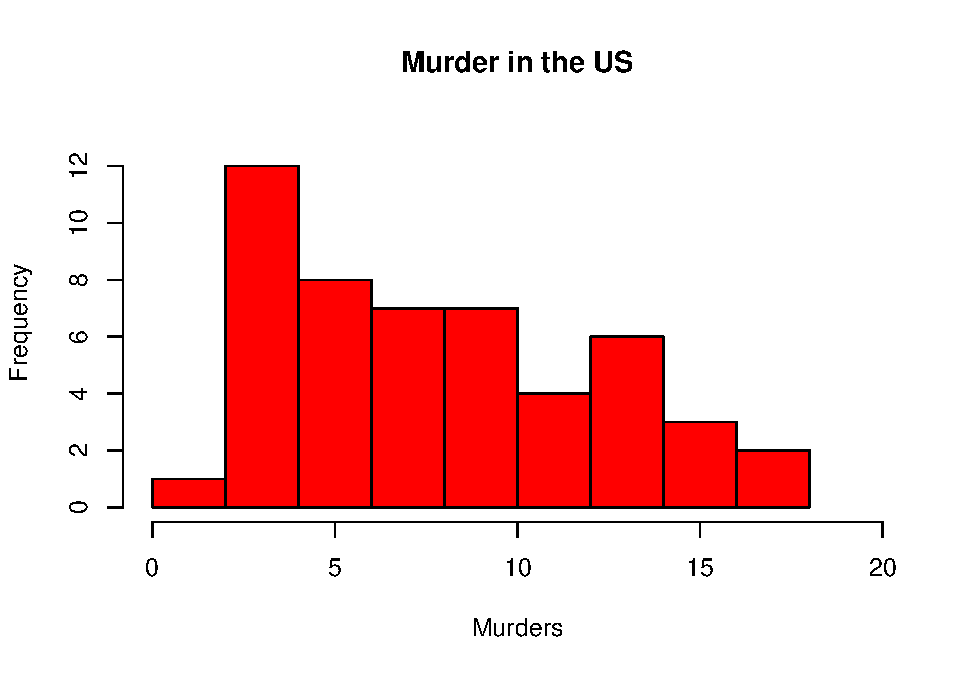
\includegraphics{Assignments_files/figure-latex/unnamed-chunk-5-1.pdf}

\hypertarget{problem-6}{%
\subsubsection{Problem 6}\label{problem-6}}

Please summarize \texttt{Murder} quantitatively. What are its mean and
median? What is the difference between mean and median? What is a
quartile, and why do you think R gives you the 1st Qu. and 3rd Qu.?

\begin{Shaded}
\begin{Highlighting}[]
\FunctionTok{summary}\NormalTok{(dat.us}\SpecialCharTok{$}\NormalTok{Murder)}
\end{Highlighting}
\end{Shaded}

\begin{verbatim}
##    Min. 1st Qu.  Median    Mean 3rd Qu.    Max. 
##   0.800   4.075   7.250   7.788  11.250  17.400
\end{verbatim}

\textbf{Answer}: The mean for Murder is 7.788 and the median is 7.250.
The mean is the amount that each subject would have if all of the values
were added together and evenly distributed. If all 50 states had the
same frequency of arrests for murders then it would be 7.788. The median
is the middle value where exactly 50\% of the values fall either above
or below it. In the US, 50\% of states have an arrest for murder
frequency above 7.250 and the other 50\% is below that. The median is
highly robust because it is not greatly affected by outliers. The mean
is the most common measure of central tendency but it is not robust
because it will change based on the skewness of the distribution. A
quartile indicates an interval that contains 25\% or a quarter of the
data.The first quartile for ``Murder'' is 4.075 which means that 25\% of
the ``Murder'' data falls below 4.075 and the 3rd quartile is 11.250
which means that 25\% of US states have a frequency of arrests for
murder that is higher than 11.250. R gives you the 1st and 3rd quartile
because those values are useful in determining the interquartile range
(IQR). The IQR is the central half which means that 50\% of the data
falls within the 1st and 3rd quartile. In a box plot, values 1.5 IQRs
above or below the tails are considered outliers.

\hypertarget{problem-7}{%
\subsubsection{Problem 7}\label{problem-7}}

Repeat the same steps you followed for \texttt{Murder}, for the
variables \texttt{Assault} and \texttt{Rape}. Now plot all three
histograms together. You can do this by using the command
\texttt{par(mfrow=c(3,1))} and then plotting each of the three.

\begin{Shaded}
\begin{Highlighting}[]
\FunctionTok{par}\NormalTok{(}\AttributeTok{mfrow=}\FunctionTok{c}\NormalTok{(}\DecValTok{3}\NormalTok{,}\DecValTok{1}\NormalTok{))}

\FunctionTok{hist}\NormalTok{(dat.us}\SpecialCharTok{$}\NormalTok{Murder, }\AttributeTok{xlab=} \StringTok{"Murders"}\NormalTok{, }\AttributeTok{ylab=}\StringTok{"Frequency"}\NormalTok{, }\AttributeTok{main=} \StringTok{"Murder in the US"}\NormalTok{, }\AttributeTok{xlim=}\NormalTok{(}\FunctionTok{c}\NormalTok{(}\DecValTok{0}\NormalTok{, }\DecValTok{20}\NormalTok{)), }\AttributeTok{ylim=}\NormalTok{(}\FunctionTok{c}\NormalTok{(}\DecValTok{0}\NormalTok{, }\DecValTok{13}\NormalTok{)), }\AttributeTok{col=}\StringTok{"red"}\NormalTok{, }\AttributeTok{breaks=} \DecValTok{10}\NormalTok{)}

\FunctionTok{hist}\NormalTok{(dat.us}\SpecialCharTok{$}\NormalTok{Assault, }\AttributeTok{xlab=} \StringTok{"Assaults"}\NormalTok{, }\AttributeTok{ylab=}\StringTok{"Frequency"}\NormalTok{, }\AttributeTok{main=} \StringTok{"Assault in the US"}\NormalTok{, }\AttributeTok{xlim=}\NormalTok{(}\FunctionTok{c}\NormalTok{(}\DecValTok{0}\NormalTok{, }\DecValTok{350}\NormalTok{)), }\AttributeTok{ylim=}\NormalTok{(}\FunctionTok{c}\NormalTok{(}\DecValTok{0}\NormalTok{, }\DecValTok{15}\NormalTok{)), }\AttributeTok{col=}\StringTok{"blue"}\NormalTok{, }\AttributeTok{breaks=}\DecValTok{10}\NormalTok{)}

\FunctionTok{hist}\NormalTok{(dat.us}\SpecialCharTok{$}\NormalTok{Rape, }\AttributeTok{xlab=} \StringTok{"Rapes"}\NormalTok{, }\AttributeTok{ylab=}\StringTok{"Frequency"}\NormalTok{, }\AttributeTok{main=} \StringTok{"Rape in the US"}\NormalTok{, }\AttributeTok{xlim=}\NormalTok{(}\FunctionTok{c}\NormalTok{(}\DecValTok{0}\NormalTok{, }\DecValTok{50}\NormalTok{)), }\AttributeTok{ylim=}\NormalTok{(}\FunctionTok{c}\NormalTok{(}\DecValTok{0}\NormalTok{, }\DecValTok{15}\NormalTok{)), }\AttributeTok{col=}\StringTok{"green"}\NormalTok{, }\AttributeTok{breaks=}\DecValTok{10}\NormalTok{)}
\end{Highlighting}
\end{Shaded}

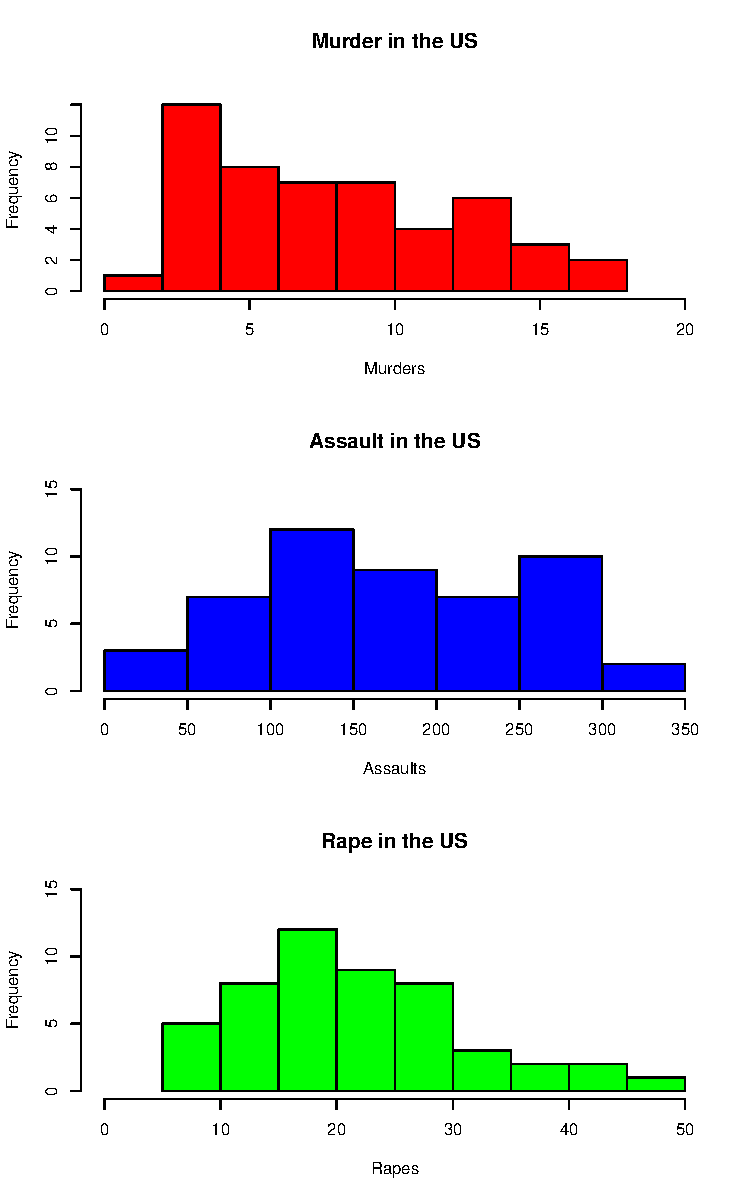
\includegraphics{Assignments_files/figure-latex/unnamed-chunk-7-1.pdf}

What does the command par do, in your own words (you can look this up by
asking R \texttt{?par})?

\textbf{Answer}: Command par is used to set parameters. The mfrow input
allows you to create an array to plot multiple graphs on one window. The
command par(mfrow=c(3,1)) allows three graphs to be plotted in three
rows.

What can you learn from plotting the histograms together?

Answer: When the histograms are plotted together it is easier to compare
the skewness and spread of each plot. You can see where each histogram
has its peaks and outliers.

\hypertarget{problem-8}{%
\subsubsection{Problem 8}\label{problem-8}}

In the console below (not in text), type
\texttt{install.packages("maps")} and press Enter, and then type
\texttt{install.packages("ggplot2")} and press Enter. This will install
the packages so you can load the libraries.

Run this code:

\begin{Shaded}
\begin{Highlighting}[]
\CommentTok{\#install.packages("maps") }
\CommentTok{\#install.packages("ggplot2")}

\FunctionTok{library}\NormalTok{(maps) }
\FunctionTok{library}\NormalTok{(ggplot2) }

\FunctionTok{ggplot}\NormalTok{(dat.us, }\FunctionTok{aes}\NormalTok{(}\AttributeTok{map\_id=}\NormalTok{state, }\AttributeTok{fill=}\NormalTok{Murder)) }\SpecialCharTok{+} 
  \FunctionTok{geom\_map}\NormalTok{(}\AttributeTok{map=}\FunctionTok{map\_data}\NormalTok{(}\StringTok{"state"}\NormalTok{)) }\SpecialCharTok{+} 
  \FunctionTok{expand\_limits}\NormalTok{(}\AttributeTok{x=}\FunctionTok{map\_data}\NormalTok{(}\StringTok{"state"}\NormalTok{)}\SpecialCharTok{$}\NormalTok{long, }\AttributeTok{y=}\FunctionTok{map\_data}\NormalTok{(}\StringTok{"state"}\NormalTok{)}\SpecialCharTok{$}\NormalTok{lat)}
\end{Highlighting}
\end{Shaded}

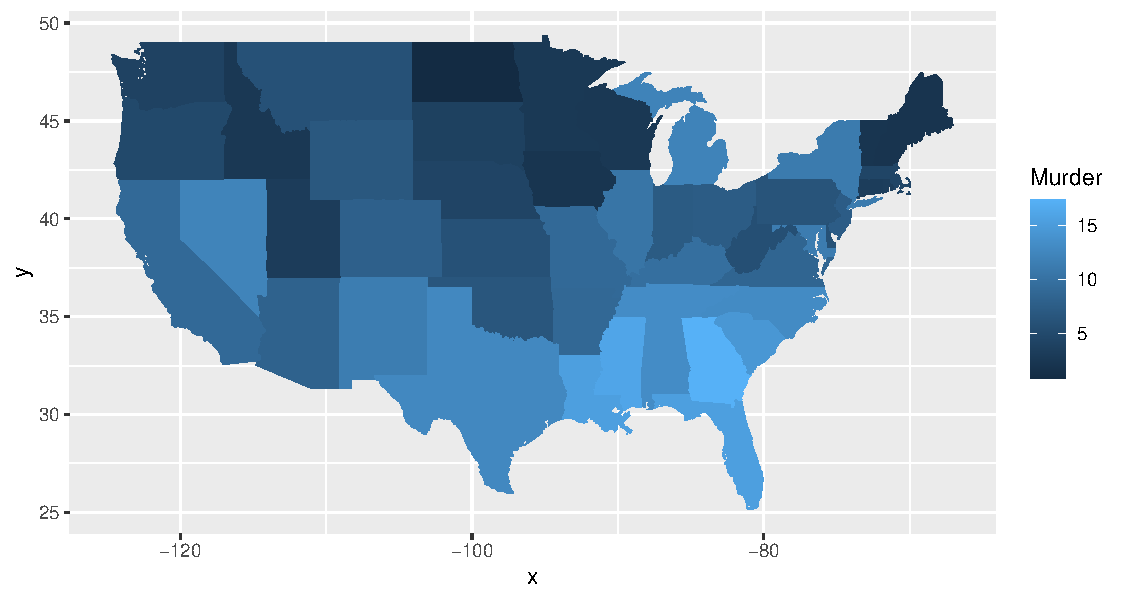
\includegraphics{Assignments_files/figure-latex/unnamed-chunk-8-1.pdf}

What does this code do? Explain what each line is doing.

Answer: The lines library(`maps') and library(`ggplot2') are pulling
from the packages that were installed. The line ggplot(dat.us,
aes(map\_id=state, fill=Murder)) is creating a ggplot with the USArrests
dataset. The plot is set with an aesthetic of a map with the US states.
Each state is filled in with its respective murder arrest data. The line
geom\_map(map=map\_data(``state'')) contains the map coordinates for
each US state.The last line
`expand\_limits(x=map\_data(``state'')\(long, y=map_data("state")\)lat)'
ensures that the limits of the plot include a single value for all
plots. The x and y axis of this plot contains the value of ``state''
from the map data. The x axis is longitude and the y axis is latitude.
Together this code creates a map of the US with each state filled in
with its value for murder arrests.The darker blue indicates that the
murder arrest frequency is 5 and below and the light blue indicates that
it is 15 and above.

\[\\[2in]\]

\hypertarget{assignment-2}{%
\section{Assignment 2}\label{assignment-2}}

\hypertarget{problem-1-1}{%
\subsubsection{Problem 1}\label{problem-1-1}}

\begin{Shaded}
\begin{Highlighting}[]
\NormalTok{dat }\OtherTok{\textless{}{-}} \FunctionTok{read.csv}\NormalTok{(}\AttributeTok{file =} \StringTok{\textquotesingle{}dat.nsduh.small.1.csv\textquotesingle{}}\NormalTok{)}


\FunctionTok{head}\NormalTok{(dat)}
\end{Highlighting}
\end{Shaded}

\begin{verbatim}
##   mjage cigage iralcage age2 sexatract speakengl irsex
## 1    14     50       14   16         1         1     1
## 2    11     14        5   13         2         1     2
## 3    12     35       12   15         2         1     2
## 4    16     18       18   14         1         1     1
## 5    14     16       14   16         4         1     1
## 6    12     16       18   15         4         1     2
\end{verbatim}

\begin{Shaded}
\begin{Highlighting}[]
\FunctionTok{names}\NormalTok{(dat)}
\end{Highlighting}
\end{Shaded}

\begin{verbatim}
## [1] "mjage"     "cigage"    "iralcage"  "age2"      "sexatract" "speakengl"
## [7] "irsex"
\end{verbatim}

\begin{Shaded}
\begin{Highlighting}[]
\FunctionTok{dim}\NormalTok{(dat)}
\end{Highlighting}
\end{Shaded}

\begin{verbatim}
## [1] 171   7
\end{verbatim}

What are the dimensions of the dataset?

\emph{Answer}: The data has 7 columns for the 7 variables (mjage,
cigage, iralcage, age2, sexatract, speakeng1 and irsex). There are 171
observations in the data.

\hypertarget{problem-2-1}{%
\subsubsection{Problem 2}\label{problem-2-1}}

Describe the variables in the dataset.

\emph{Answer}:There are 7 variables in the dataset. mjage represents the
age whne the participants first used marijuana or hashish. Cigage
represents the age when the participants first started smoking
cigarettes everyday. Iralcage is the age when participants first tried
alcohol. Age2 is the final edited age of the participants. Irsex
represents the gender of participants. Sexatract is the sexual
attraction of the participants. Speakeng represents how well the
participant speaks english.

What is this dataset about? Who collected the data, what kind of sample
is it, and what was the purpose of generating the data?

\emph{Answer}:This dataset is a small sample from the 2019 survey from
the National Survey of Drug Use and Health about drug use in the 50
states and the District of Columbia in the United States. The survey was
directed by the Sibstance Abuse and Mental Health Services
Administration and it was conducted by RTI International. The survey is
used to determine which populations and geographic areas have particular
substance use problems so federal resources can be used effectivly.

\hypertarget{problem-3-age-and-gender}{%
\subsubsection{Problem 3: Age and
gender}\label{problem-3-age-and-gender}}

What is the age distribution of the sample like? Make sure you read the
codebook to know what the variable values mean.

\begin{Shaded}
\begin{Highlighting}[]
\FunctionTok{hist}\NormalTok{(dat}\SpecialCharTok{$}\NormalTok{age2, }\AttributeTok{xlab=} \StringTok{"Final Edited Age"}\NormalTok{, }\AttributeTok{main=} \StringTok{"Age Distribution of NSDUH 2019 Survey"}\NormalTok{, }\AttributeTok{col=}\StringTok{"purple"}\NormalTok{)}
\end{Highlighting}
\end{Shaded}

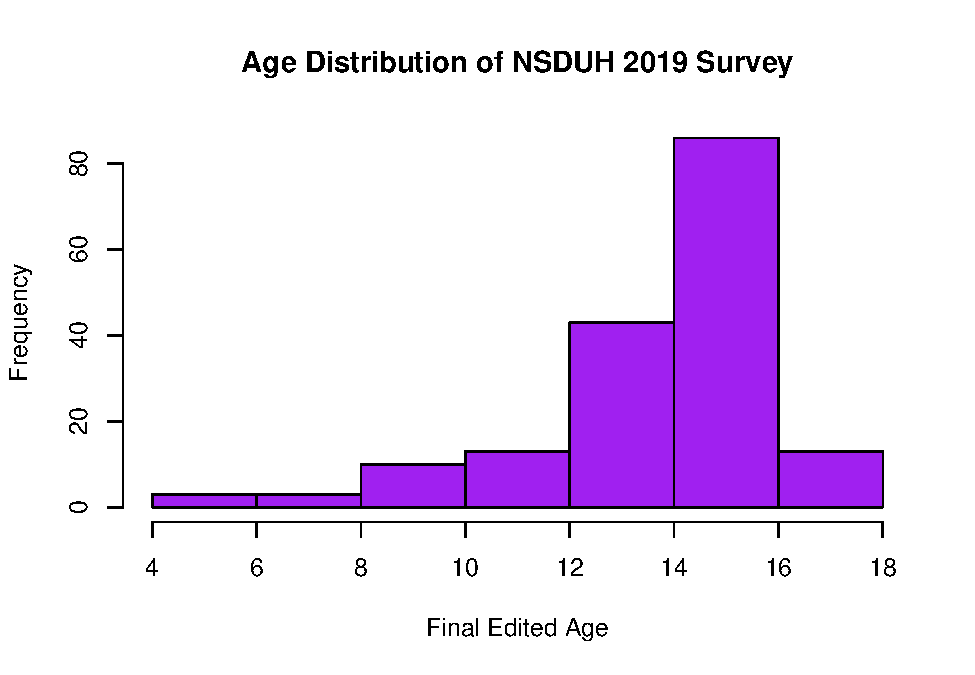
\includegraphics{Assignments_files/figure-latex/unnamed-chunk-10-1.pdf}

\emph{Answer}:The age distribution is negatively skewed because the bulk
of the data is in the upper range with thin tails in the lower range.
This shows that most of the respondents of the survey were 25 years old
to greater than 65 years old. This age variable is categorical because
the numbers represent categories of age for example 12 indicates that
the respondent is 24 or 25 years old.

Do you think this age distribution representative of the US population?
Why or why not?

\emph{Answer}:I do not think this age distribution is representative of
the US population because while the households chosen for the survey are
randomly selected, only one person per household can respond to the
survey and the interviews are completed online and not every person in
the US has access to a computer or internet. There is also a money
incentive to complete the survey.It is possible that more middle aged
people responded to the survey.

Is the sample balanced in terms of gender? If not, are there more
females or males?

Use this code to draw a stacked bar plot to view the relationship
between sex and age. What can you conclude from this plot?

\begin{Shaded}
\begin{Highlighting}[]
\NormalTok{tab.agesex }\OtherTok{\textless{}{-}} \FunctionTok{table}\NormalTok{(dat}\SpecialCharTok{$}\NormalTok{irsex, dat}\SpecialCharTok{$}\NormalTok{age2)}
\FunctionTok{barplot}\NormalTok{(tab.agesex,}
        \AttributeTok{main =} \StringTok{"Stacked barchart"}\NormalTok{,}
        \AttributeTok{xlab =} \StringTok{"Age category"}\NormalTok{, }\AttributeTok{ylab =} \StringTok{"Frequency"}\NormalTok{,}
        \AttributeTok{legend.text =} \FunctionTok{rownames}\NormalTok{(tab.agesex),}
        \AttributeTok{beside =} \ConstantTok{FALSE}\NormalTok{) }
\end{Highlighting}
\end{Shaded}

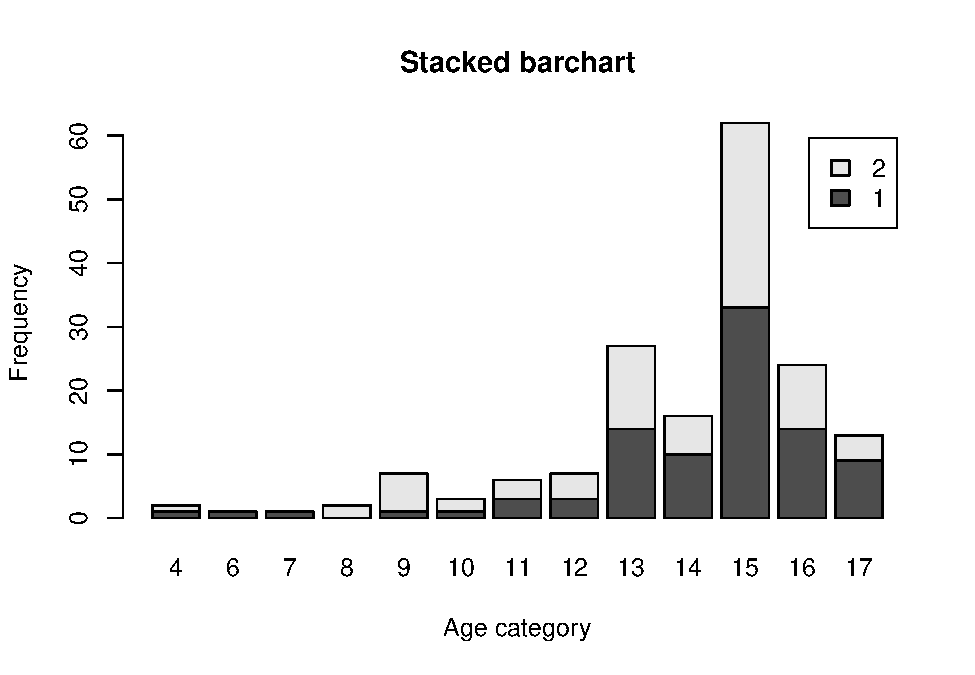
\includegraphics{Assignments_files/figure-latex/unnamed-chunk-11-1.pdf}

\emph{Answer}:The sample is not fully balanced in terms of gender. There
are more females with 52.28\% of respondents being female and 47.72\%
being male.

\emph{Answer}:From this plot, we can determine that the relationship
between sex and age is fairly even. For the largest age group, the
gender distribution appears to be almost equal. However, for the lower
age groups there appears to be more female respondents and for the
higher age distributions there appears to be more male respondents.

\hypertarget{problem-4-substance-use}{%
\subsubsection{Problem 4: Substance use}\label{problem-4-substance-use}}

For which of the three substances included in the dataset (marijuana,
alcohol, and cigarettes) do individuals tend to use the substance
earlier?

\begin{Shaded}
\begin{Highlighting}[]
\FunctionTok{par}\NormalTok{(}\AttributeTok{mfrow=}\FunctionTok{c}\NormalTok{(}\DecValTok{3}\NormalTok{,}\DecValTok{1}\NormalTok{))}

\FunctionTok{hist}\NormalTok{(dat}\SpecialCharTok{$}\NormalTok{mjage, }\AttributeTok{col=}\StringTok{"green"}\NormalTok{, }\AttributeTok{xlab=} \StringTok{"Age of first Marijuana Use"}\NormalTok{, }\AttributeTok{main=} \StringTok{"Age Distribution of First Marijuana Use"}\NormalTok{, }\AttributeTok{xlim=} \FunctionTok{c}\NormalTok{(}\DecValTok{0}\NormalTok{,}\DecValTok{50}\NormalTok{), }\AttributeTok{ylim=} \FunctionTok{c}\NormalTok{(}\DecValTok{0}\NormalTok{,}\DecValTok{100}\NormalTok{)) }

\FunctionTok{hist}\NormalTok{(dat}\SpecialCharTok{$}\NormalTok{cigage, }\AttributeTok{col=}\StringTok{"grey"}\NormalTok{, }\AttributeTok{xlab=} \StringTok{"Age of first Cigarette Use"}\NormalTok{, }\AttributeTok{main=} \StringTok{"Age Distribution of First Cigarette Use"}\NormalTok{, }\AttributeTok{xlim=} \FunctionTok{c}\NormalTok{(}\DecValTok{0}\NormalTok{,}\DecValTok{50}\NormalTok{), }\AttributeTok{ylim=} \FunctionTok{c}\NormalTok{(}\DecValTok{0}\NormalTok{,}\DecValTok{100}\NormalTok{)) }

\FunctionTok{hist}\NormalTok{(dat}\SpecialCharTok{$}\NormalTok{iralcage, }\AttributeTok{col=}\StringTok{"orange"}\NormalTok{, }\AttributeTok{xlab=} \StringTok{"Age of first Alcohol Use"}\NormalTok{, }\AttributeTok{main=} \StringTok{"Age Distribution of First Alcohol Use"}\NormalTok{, }\AttributeTok{xlim=} \FunctionTok{c}\NormalTok{(}\DecValTok{0}\NormalTok{,}\DecValTok{50}\NormalTok{), }\AttributeTok{ylim=} \FunctionTok{c}\NormalTok{(}\DecValTok{0}\NormalTok{,}\DecValTok{100}\NormalTok{)) }
\end{Highlighting}
\end{Shaded}

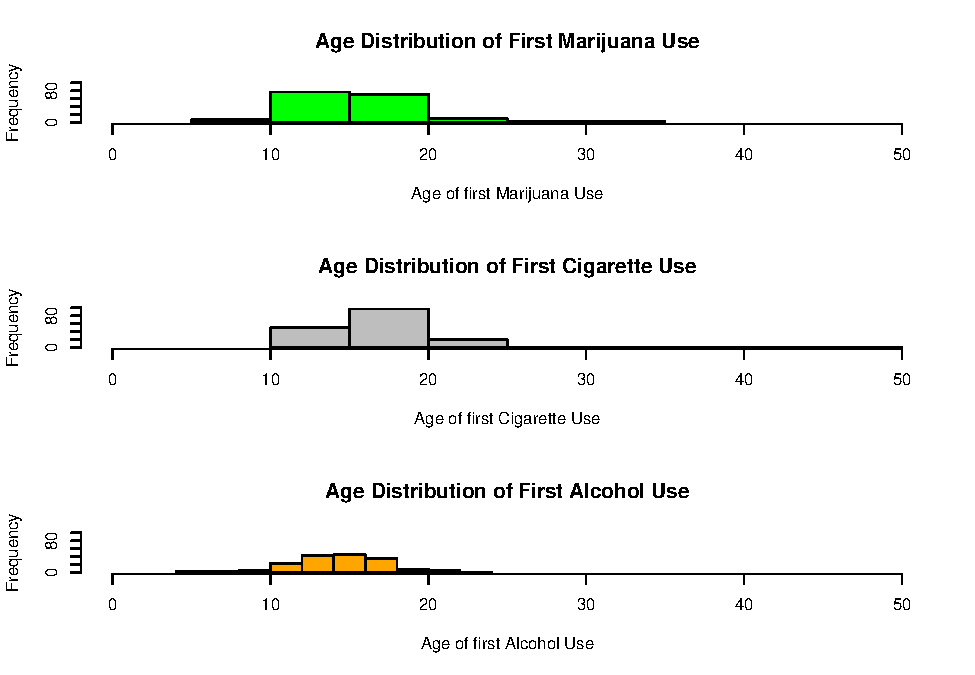
\includegraphics{Assignments_files/figure-latex/unnamed-chunk-12-1.pdf}

\emph{Answer}:Individuals tend to first start using marijuana and
alcohol at a much younger age than cigarettes but individuals tend to
first start using alcohol earliest.

\hypertarget{problem-5-sexual-attraction}{%
\subsubsection{Problem 5: Sexual
attraction}\label{problem-5-sexual-attraction}}

What does the distribution of sexual attraction look like? Is this what
you expected?

\begin{Shaded}
\begin{Highlighting}[]
\NormalTok{tab.sexatract }\OtherTok{\textless{}{-}} \FunctionTok{table}\NormalTok{(dat}\SpecialCharTok{$}\NormalTok{sexatract)}
\FunctionTok{barplot}\NormalTok{(tab.sexatract, }\AttributeTok{main=} \StringTok{"Sexual Attraction Distribution"}\NormalTok{, }\AttributeTok{xlab=} \StringTok{"Sexual Attraction"}\NormalTok{, }\AttributeTok{ylab=} \StringTok{"Frequency"}\NormalTok{)}
\end{Highlighting}
\end{Shaded}

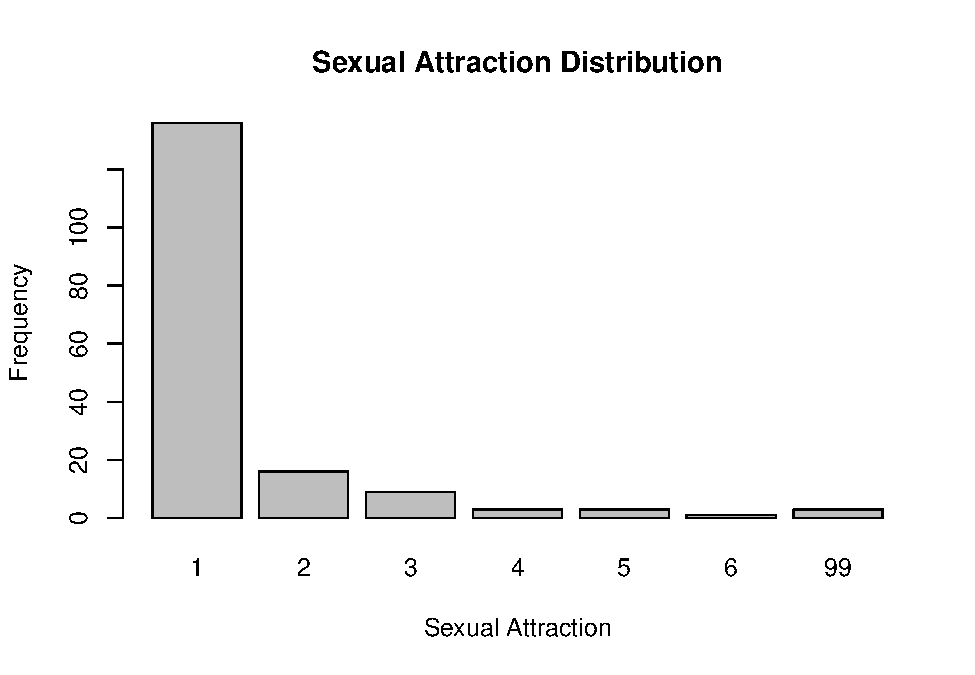
\includegraphics{Assignments_files/figure-latex/unnamed-chunk-13-1.pdf}

\emph{Answer}:Most participants are only attracted to the opposite sex.
This is expected because respondents might not have felt comfortable
answering this question unless they were only attracted to the same sex
since there is stigma for different sexual attractions. The ``99''
category is significant because a large portion of respondents (23.87\%)
skipped this question which could indicate that people were not
comfortable answering this question.

What is the distribution of sexual attraction by gender?

\begin{Shaded}
\begin{Highlighting}[]
\NormalTok{tab.sexatractsex }\OtherTok{\textless{}{-}} \FunctionTok{table}\NormalTok{(dat}\SpecialCharTok{$}\NormalTok{irsex, dat}\SpecialCharTok{$}\NormalTok{sexatract)}
\FunctionTok{barplot}\NormalTok{(tab.sexatractsex,}
        \AttributeTok{main =} \StringTok{"Stacked barchart"}\NormalTok{,}
        \AttributeTok{xlab =} \StringTok{"Age category"}\NormalTok{, }\AttributeTok{ylab =} \StringTok{"Frequency"}\NormalTok{,}
        \AttributeTok{legend.text =} \FunctionTok{rownames}\NormalTok{(tab.sexatractsex),}
        \AttributeTok{beside =} \ConstantTok{FALSE}\NormalTok{) }
\end{Highlighting}
\end{Shaded}

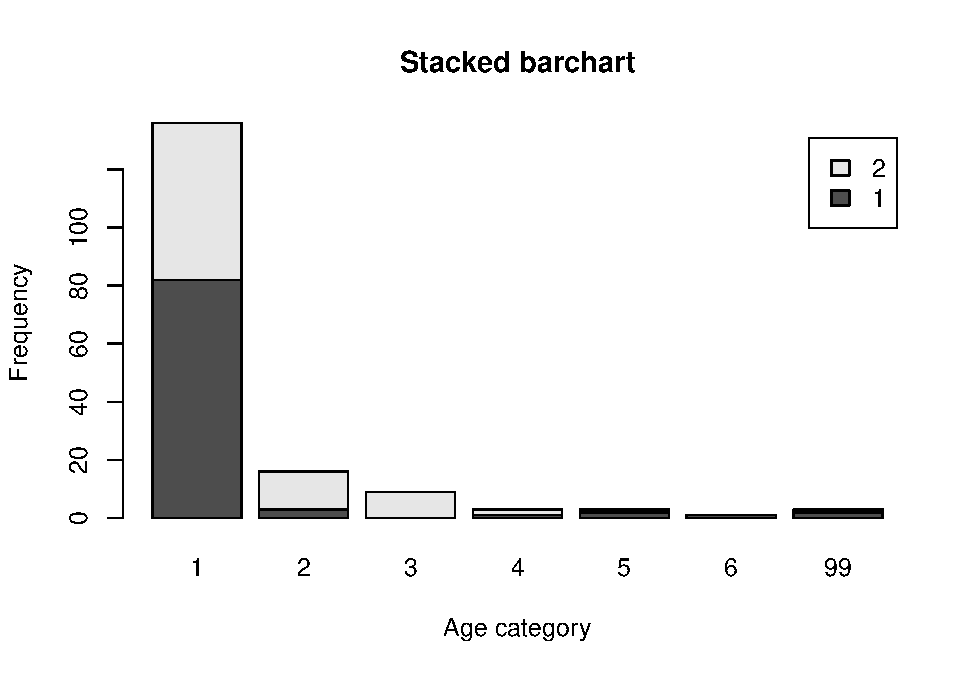
\includegraphics{Assignments_files/figure-latex/unnamed-chunk-14-1.pdf}

\hypertarget{problem-6-english-speaking}{%
\subsubsection{Problem 6: English
speaking}\label{problem-6-english-speaking}}

What does the distribution of English speaking look like in the sample?
Is this what you might expect for a random sample of the US population?

\begin{Shaded}
\begin{Highlighting}[]
\NormalTok{tab.speakeng }\OtherTok{\textless{}{-}} \FunctionTok{table}\NormalTok{(dat}\SpecialCharTok{$}\NormalTok{speakengl)}
\FunctionTok{barplot}\NormalTok{(tab.speakeng, }\AttributeTok{xlab=} \StringTok{"How Well English is Spoken"}\NormalTok{, }\AttributeTok{ylab=} \StringTok{"Frequency"}\NormalTok{, }\AttributeTok{names.arg =} \FunctionTok{c}\NormalTok{(}\StringTok{"Very Well"}\NormalTok{,}\StringTok{"Well"}\NormalTok{,}\StringTok{"Not Well"}\NormalTok{), }\AttributeTok{main =} \StringTok{"Distribution of English Speaking"}\NormalTok{)}
\end{Highlighting}
\end{Shaded}

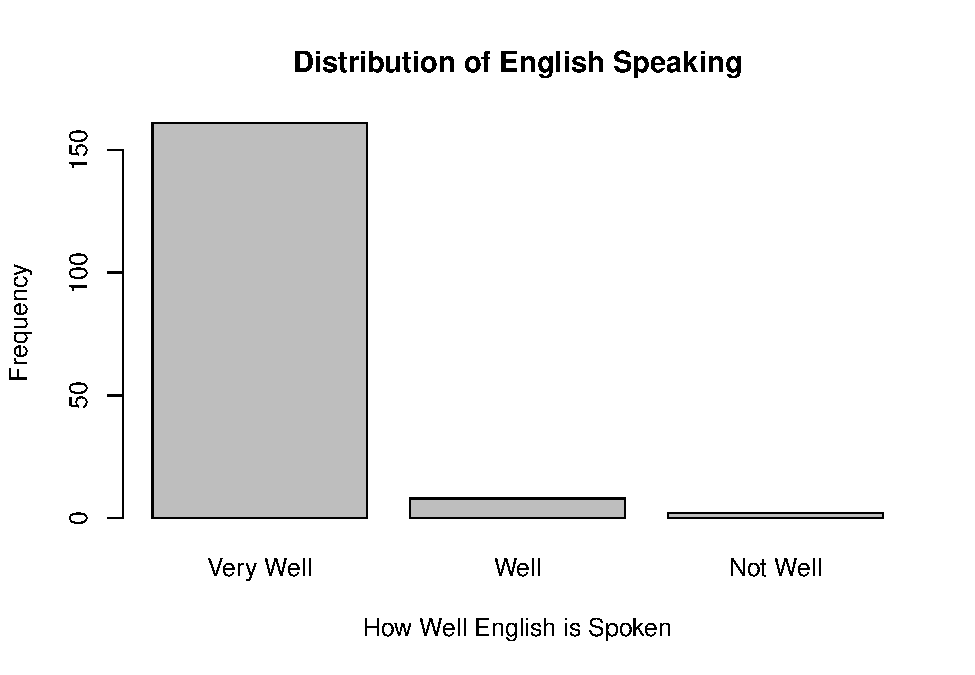
\includegraphics{Assignments_files/figure-latex/unnamed-chunk-15-1.pdf}

\emph{Answer}:Most of the participants speak English very well which is
expected because for the most part the US is an english speaking
country. It might have been hard for non-english speakers to engage with
the survey if interpreters or different language options were not
available.

Are there more English speaker females or males?

\begin{Shaded}
\begin{Highlighting}[]
\NormalTok{tab.speakengsex }\OtherTok{\textless{}{-}} \FunctionTok{table}\NormalTok{(dat}\SpecialCharTok{$}\NormalTok{irsex, dat}\SpecialCharTok{$}\NormalTok{speakengl)}
\FunctionTok{barplot}\NormalTok{(tab.speakengsex,}
        \AttributeTok{main =} \StringTok{"Stacked barchart"}\NormalTok{,}
        \AttributeTok{xlab =} \StringTok{"Age category"}\NormalTok{, }\AttributeTok{ylab =} \StringTok{"Frequency"}\NormalTok{,}
        \AttributeTok{legend.text =} \FunctionTok{rownames}\NormalTok{(tab.speakengsex),}
        \AttributeTok{beside =} \ConstantTok{FALSE}\NormalTok{) }
\end{Highlighting}
\end{Shaded}

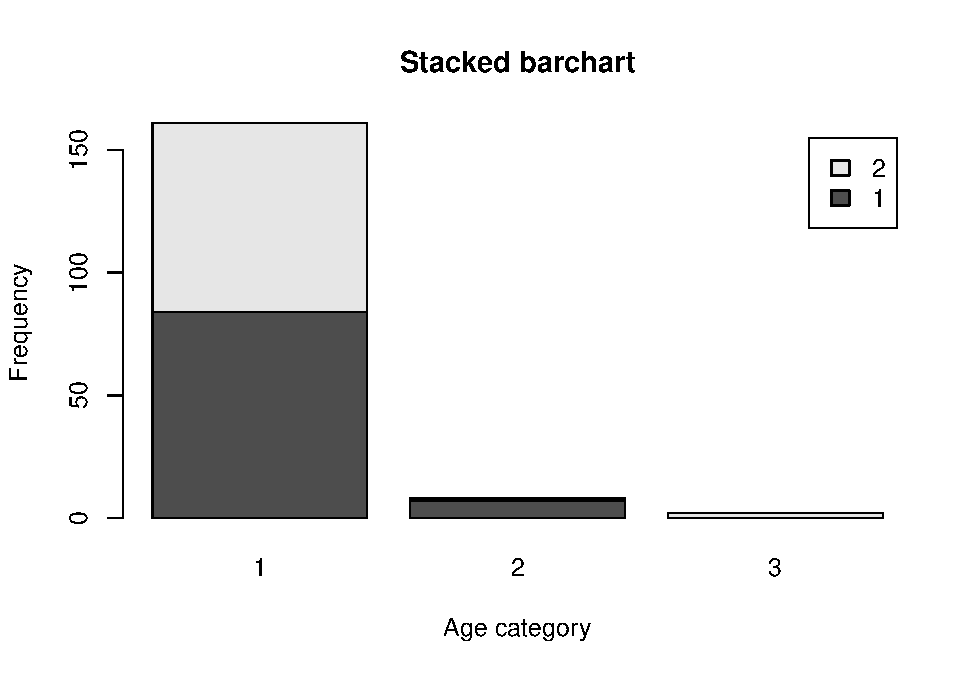
\includegraphics{Assignments_files/figure-latex/unnamed-chunk-16-1.pdf}

\emph{Answer}:There appears to be an equal amount of English speaking
females and males.

\[\\[2in]\]

\hypertarget{exam-1}{%
\section{Exam 1}\label{exam-1}}

Load the data into an R data frame.

\begin{Shaded}
\begin{Highlighting}[]
\CommentTok{\#read.csv(file = \textquotesingle{}fatal{-}police{-}shootings{-}data.csv\textquotesingle{})}
\NormalTok{dat }\OtherTok{\textless{}{-}} \FunctionTok{read.csv}\NormalTok{(}\AttributeTok{file =} \StringTok{\textquotesingle{}fatal{-}police{-}shootings{-}data.csv\textquotesingle{}}\NormalTok{)}

\FunctionTok{head}\NormalTok{(dat)}
\end{Highlighting}
\end{Shaded}

\begin{verbatim}
##   id               name       date  manner_of_death      armed age gender race
## 1  3         Tim Elliot 2015-01-02             shot        gun  53      M    A
## 2  4   Lewis Lee Lembke 2015-01-02             shot        gun  47      M    W
## 3  5 John Paul Quintero 2015-01-03 shot and Tasered    unarmed  23      M    H
## 4  8    Matthew Hoffman 2015-01-04             shot toy weapon  32      M    W
## 5  9  Michael Rodriguez 2015-01-04             shot   nail gun  39      M    H
## 6 11  Kenneth Joe Brown 2015-01-04             shot        gun  18      M    W
##            city state signs_of_mental_illness threat_level        flee
## 1       Shelton    WA                    True       attack Not fleeing
## 2         Aloha    OR                   False       attack Not fleeing
## 3       Wichita    KS                   False        other Not fleeing
## 4 San Francisco    CA                    True       attack Not fleeing
## 5         Evans    CO                   False       attack Not fleeing
## 6       Guthrie    OK                   False       attack Not fleeing
##   body_camera longitude latitude is_geocoding_exact
## 1       False  -123.122   47.247               True
## 2       False  -122.892   45.487               True
## 3       False   -97.281   37.695               True
## 4       False  -122.422   37.763               True
## 5       False  -104.692   40.384               True
## 6       False   -97.423   35.877               True
\end{verbatim}

\hypertarget{problem-1-2}{%
\subsubsection{Problem 1}\label{problem-1-2}}

\begin{enumerate}
\def\labelenumi{\alph{enumi}.}
\tightlist
\item
  Describe the dataset. This is the source:
  \url{https://github.com/washingtonpost/data-police-shootings} . Write
  two sentences (max.) about this.
\end{enumerate}

\textbf{This dataset contains the data of fatal police shootings of
civilians in 2015. The data was collected from the Washington Post using
local news reports, law enforcement websites, social media and
independent databases.}

\begin{enumerate}
\def\labelenumi{\alph{enumi}.}
\setcounter{enumi}{1}
\tightlist
\item
  How many observations are there in the data frame?
\end{enumerate}

\begin{Shaded}
\begin{Highlighting}[]
\FunctionTok{dim}\NormalTok{(dat)}
\end{Highlighting}
\end{Shaded}

\begin{verbatim}
## [1] 6594   17
\end{verbatim}

\textbf{There are 6594 rows (observations) in the dataset with 17
columns. }

\begin{enumerate}
\def\labelenumi{\alph{enumi}.}
\setcounter{enumi}{2}
\tightlist
\item
  Look at the names of the variables in the data frame. Describe what
  ``body\_camera'', ``flee'', and ``armed'' represent, according to the
  codebook. Again, only write one sentence (max) per variable.
\end{enumerate}

\begin{Shaded}
\begin{Highlighting}[]
\FunctionTok{names}\NormalTok{(dat)}
\end{Highlighting}
\end{Shaded}

\begin{verbatim}
##  [1] "id"                      "name"                   
##  [3] "date"                    "manner_of_death"        
##  [5] "armed"                   "age"                    
##  [7] "gender"                  "race"                   
##  [9] "city"                    "state"                  
## [11] "signs_of_mental_illness" "threat_level"           
## [13] "flee"                    "body_camera"            
## [15] "longitude"               "latitude"               
## [17] "is_geocoding_exact"
\end{verbatim}

\textbf{The variable ``body\_camera indicates that the police officer
was wearing a body camera and may have recorded some parts of the
incident. The variable''flee" means that the victim was moving away from
the officers. The variable ``armed'' means that victim had an instrument
that the police believed could inflict harm. }

\begin{enumerate}
\def\labelenumi{\alph{enumi}.}
\setcounter{enumi}{3}
\tightlist
\item
  What are three weapons that you are surprised to find in the ``armed''
  variable? Make a table of the values in ``armed'' to see the options.
\end{enumerate}

\begin{Shaded}
\begin{Highlighting}[]
\FunctionTok{table}\NormalTok{(dat}\SpecialCharTok{$}\NormalTok{armed)}
\end{Highlighting}
\end{Shaded}

\begin{verbatim}
## 
##                                                   air conditioner 
##                              207                                1 
##                       air pistol                   Airsoft pistol 
##                                1                                3 
##                               ax                         barstool 
##                               24                                1 
##                     baseball bat          baseball bat and bottle 
##                               20                                1 
## baseball bat and fireplace poker           baseball bat and knife 
##                                1                                1 
##                            baton                           BB gun 
##                                6                               15 
##               BB gun and vehicle                     bean-bag gun 
##                                1                                1 
##                      beer bottle                       binoculars 
##                                3                                1 
##                     blunt object                           bottle 
##                                5                                1 
##                    bow and arrow                       box cutter 
##                                1                               13 
##                            brick              car, knife and mace 
##                                2                                1 
##                          carjack                            chain 
##                                1                                3 
##                        chain saw                         chainsaw 
##                                2                                1 
##                            chair              claimed to be armed 
##                                4                                1 
##               contractor's level                   cordless drill 
##                                1                                1 
##                         crossbow                          crowbar 
##                                9                                5 
##                        fireworks                         flagpole 
##                                1                                1 
##                       flashlight                      garden tool 
##                                2                                2 
##                      glass shard                          grenade 
##                                4                                1 
##                              gun                      gun and car 
##                             3798                               12 
##                    gun and knife                  gun and machete 
##                               22                                3 
##                    gun and sword                  gun and vehicle 
##                                1                               17 
##              guns and explosives                           hammer 
##                                3                               18 
##                       hand torch                          hatchet 
##                                1                               14 
##                  hatchet and gun                         ice pick 
##                                2                                1 
##                incendiary device                            knife 
##                                2                              955 
##                knife and vehicle                 lawn mower blade 
##                                1                                2 
##                          machete                  machete and gun 
##                               51                                1 
##                     meat cleaver                  metal hand tool 
##                                6                                2 
##                     metal object                       metal pipe 
##                                5                               16 
##                       metal pole                       metal rake 
##                                4                                1 
##                      metal stick                       microphone 
##                                3                                1 
##                       motorcycle                         nail gun 
##                                1                                1 
##                              oar                       pellet gun 
##                                1                                3 
##                              pen                     pepper spray 
##                                1                                2 
##                         pick-axe                    piece of wood 
##                                4                                7 
##                             pipe                        pitchfork 
##                                7                                2 
##                             pole                   pole and knife 
##                                3                                2 
##                  railroad spikes                             rock 
##                                1                                7 
##                    samurai sword                         scissors 
##                                4                                9 
##                      screwdriver                     sharp object 
##                               16                               14 
##                           shovel                            spear 
##                                7                                2 
##                          stapler              straight edge razor 
##                                1                                5 
##                            sword                            Taser 
##                               23                               34 
##                        tire iron                       toy weapon 
##                                4                              226 
##                          unarmed                     undetermined 
##                              421                              188 
##                   unknown weapon                          vehicle 
##                               82                              213 
##                  vehicle and gun              vehicle and machete 
##                                8                                1 
##                    walking stick                       wasp spray 
##                                1                                1 
##                           wrench 
##                                1
\end{verbatim}

\textbf{I am suprised to see air conditioner, flashlight and stapler in
the ``armed'' variable.}

\hypertarget{problem-2-2}{%
\subsubsection{Problem 2}\label{problem-2-2}}

\begin{enumerate}
\def\labelenumi{\alph{enumi}.}
\tightlist
\item
  Describe the age distribution of the sample. Is this what you would
  expect to see?
\end{enumerate}

\begin{Shaded}
\begin{Highlighting}[]
\FunctionTok{hist}\NormalTok{(dat}\SpecialCharTok{$}\NormalTok{age, }\AttributeTok{main=} \StringTok{"Age Distribution of Fatal Police Shootings"}\NormalTok{, }\AttributeTok{xlab=}\StringTok{"Age of Victims"}\NormalTok{, }\AttributeTok{ylab=} \StringTok{"Frequency"}\NormalTok{, }\AttributeTok{xlim=}\NormalTok{(}\FunctionTok{c}\NormalTok{(}\DecValTok{0}\NormalTok{,}\DecValTok{100}\NormalTok{)))}
\end{Highlighting}
\end{Shaded}

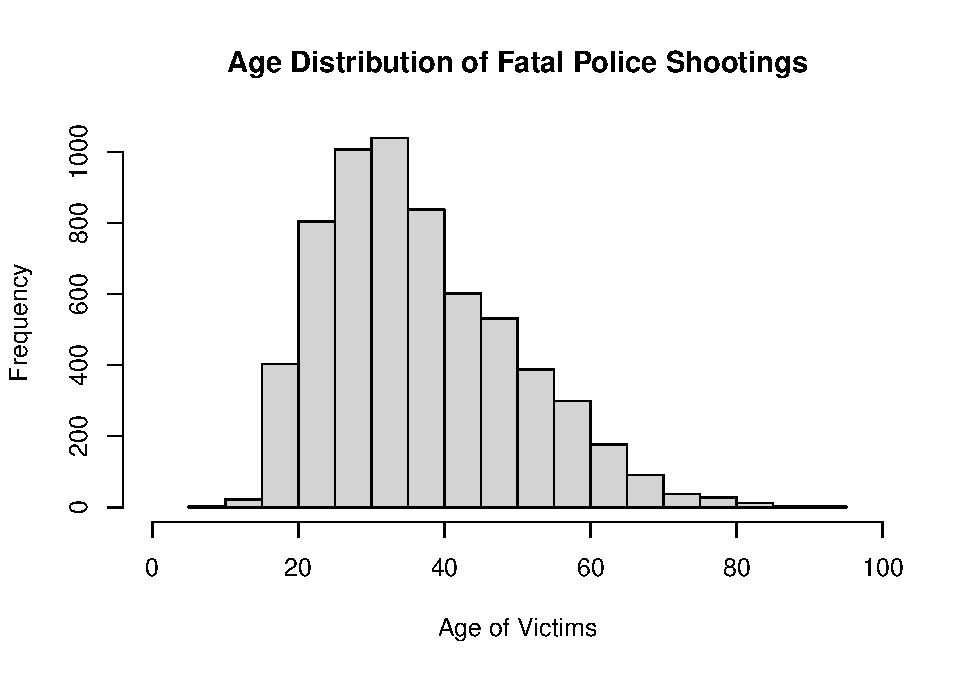
\includegraphics{Assignments_files/figure-latex/unnamed-chunk-21-1.pdf}

\textbf{The distribution of age is skewed to the right. There are some
missing values in this distribution. The bulk of the victims were under
the age of 40 which makes sense because younger people tend to encounter
the police more since they are expected to commit more crimes.}

\begin{enumerate}
\def\labelenumi{\alph{enumi}.}
\setcounter{enumi}{1}
\tightlist
\item
  To understand the center of the age distribution, would you use a mean
  or a median, and why? Find the one you picked.
\end{enumerate}

\begin{Shaded}
\begin{Highlighting}[]
\FunctionTok{summary}\NormalTok{(dat}\SpecialCharTok{$}\NormalTok{age)}
\end{Highlighting}
\end{Shaded}

\begin{verbatim}
##    Min. 1st Qu.  Median    Mean 3rd Qu.    Max.    NA's 
##    6.00   27.00   35.00   37.12   45.00   91.00     308
\end{verbatim}

\textbf{Since the age distribution is not a normal bell curve then the
median would be a better estimate of the center of the distribution
since it is more resistant to skewness.The median of the distribution is
35 years old.}

\begin{enumerate}
\def\labelenumi{\alph{enumi}.}
\setcounter{enumi}{2}
\tightlist
\item
  Describe the gender distribution of the sample. Do you find this
  surprising?
\end{enumerate}

\begin{Shaded}
\begin{Highlighting}[]
\FunctionTok{table}\NormalTok{(dat}\SpecialCharTok{$}\NormalTok{gender)}
\end{Highlighting}
\end{Shaded}

\begin{verbatim}
## 
##         F    M 
##    3  293 6298
\end{verbatim}

\begin{Shaded}
\begin{Highlighting}[]
\NormalTok{dat}\SpecialCharTok{$}\NormalTok{gender.nas }\OtherTok{\textless{}{-}} \FunctionTok{ifelse}\NormalTok{(dat}\SpecialCharTok{$}\NormalTok{gender}\SpecialCharTok{==}\StringTok{""}\NormalTok{, }\ConstantTok{NA}\NormalTok{, dat}\SpecialCharTok{$}\NormalTok{gender)}
\FunctionTok{table}\NormalTok{(dat}\SpecialCharTok{$}\NormalTok{gender.nas)}
\end{Highlighting}
\end{Shaded}

\begin{verbatim}
## 
##    F    M 
##  293 6298
\end{verbatim}

\begin{Shaded}
\begin{Highlighting}[]
\NormalTok{gender.no.nas }\OtherTok{\textless{}{-}} \FunctionTok{na.omit}\NormalTok{(dat}\SpecialCharTok{$}\NormalTok{gender.nas)}
\FunctionTok{table}\NormalTok{(gender.no.nas)}
\end{Highlighting}
\end{Shaded}

\begin{verbatim}
## gender.no.nas
##    F    M 
##  293 6298
\end{verbatim}

\begin{Shaded}
\begin{Highlighting}[]
\NormalTok{tab.gender }\OtherTok{\textless{}{-}} \FunctionTok{table}\NormalTok{(gender.no.nas)}
\FunctionTok{barplot}\NormalTok{(tab.gender, }\AttributeTok{main=} \StringTok{"Gender Distribution of Fatal Police Shootings"}\NormalTok{, }\AttributeTok{xlab=} \StringTok{"Gender"}\NormalTok{, }\AttributeTok{ylab=}\StringTok{"Frequency"}\NormalTok{)}
\end{Highlighting}
\end{Shaded}

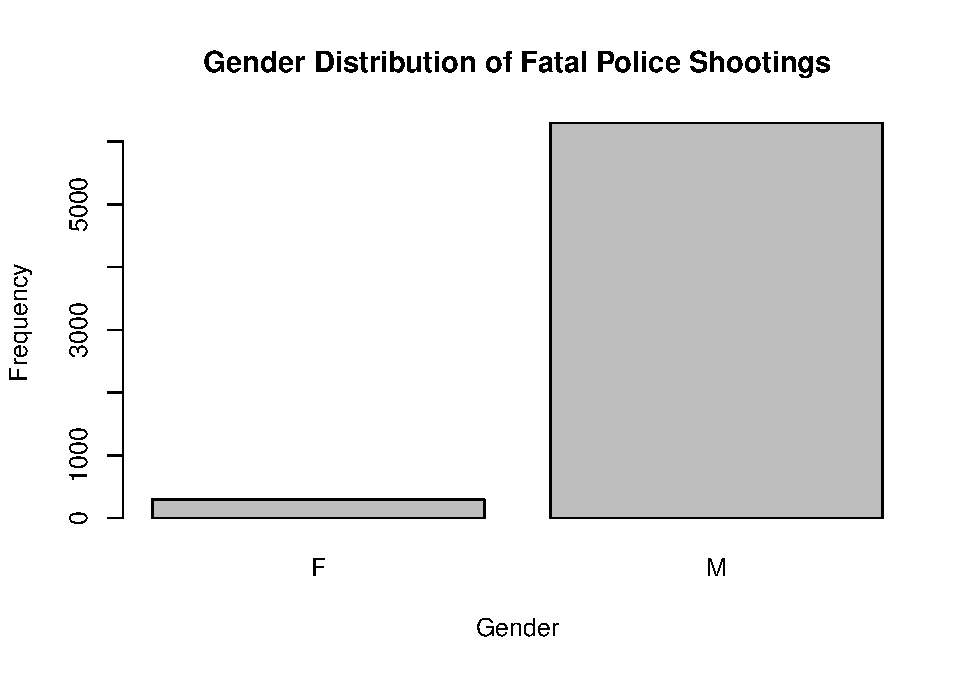
\includegraphics{Assignments_files/figure-latex/unnamed-chunk-23-1.pdf}

\textbf{The majority of fatal police shooting victims were males. This
is expected because the majority of people targeted by the police are
males.Missing values were omitted from the distribution because the
gender of those victims were unknown.}

\hypertarget{problem-3-1}{%
\subsubsection{Problem 3}\label{problem-3-1}}

\begin{enumerate}
\def\labelenumi{\alph{enumi}.}
\tightlist
\item
  How many police officers had a body camera, according to news reports?
  What proportion is this of all the incidents in the data? Are you
  surprised that it is so high or low?
\end{enumerate}

\begin{Shaded}
\begin{Highlighting}[]
\FunctionTok{table}\NormalTok{(dat}\SpecialCharTok{$}\NormalTok{body\_camera)}
\end{Highlighting}
\end{Shaded}

\begin{verbatim}
## 
## False  True 
##  5684   910
\end{verbatim}

\begin{Shaded}
\begin{Highlighting}[]
\FunctionTok{prop.table}\NormalTok{(}\FunctionTok{table}\NormalTok{(dat}\SpecialCharTok{$}\NormalTok{body\_camera))}
\end{Highlighting}
\end{Shaded}

\begin{verbatim}
## 
##     False      True 
## 0.8619958 0.1380042
\end{verbatim}

\textbf{910 police officers had a body camera according to news
reports.This is around 14\% of all the incidents in the data. I am
surprised that it is so low because I assumed that body cameras have
become a norm for police stations but they are expensive and some
precincts are not strict with body cameras.}

\begin{enumerate}
\def\labelenumi{\alph{enumi}.}
\setcounter{enumi}{1}
\tightlist
\item
  In how many of the incidents was the victim fleeing? What proportion
  is this of the total number of incidents in the data? Is this what you
  would expect?
\end{enumerate}

\begin{Shaded}
\begin{Highlighting}[]
\FunctionTok{table}\NormalTok{(dat}\SpecialCharTok{$}\NormalTok{flee)}
\end{Highlighting}
\end{Shaded}

\begin{verbatim}
## 
##                     Car        Foot Not fleeing       Other 
##         491        1058         845        3952         248
\end{verbatim}

\begin{Shaded}
\begin{Highlighting}[]
\FunctionTok{barplot}\NormalTok{(}\FunctionTok{table}\NormalTok{(dat}\SpecialCharTok{$}\NormalTok{flee))}
\end{Highlighting}
\end{Shaded}

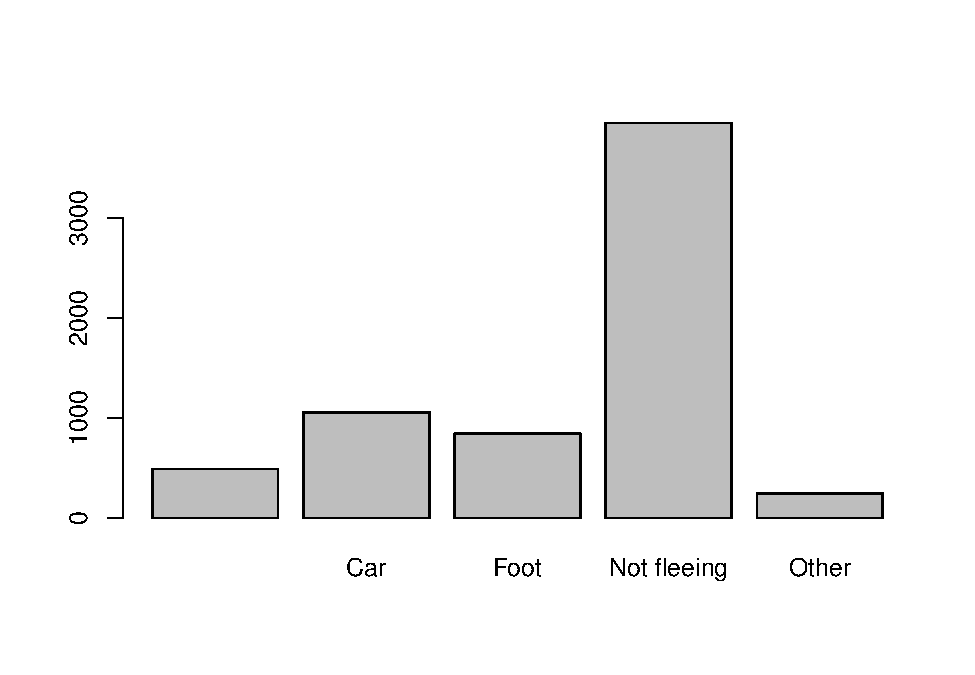
\includegraphics{Assignments_files/figure-latex/unnamed-chunk-25-1.pdf}

\begin{Shaded}
\begin{Highlighting}[]
\FunctionTok{prop.table}\NormalTok{(}\FunctionTok{table}\NormalTok{(dat}\SpecialCharTok{$}\NormalTok{flee))}
\end{Highlighting}
\end{Shaded}

\begin{verbatim}
## 
##                     Car        Foot Not fleeing       Other 
##  0.07446163  0.16044889  0.12814680  0.59933273  0.03760995
\end{verbatim}

\textbf{In 1903 incidents the victim was fleeing.This is about 29\% of
the data. This variable is a bit confusing because of the missing values
and the ``other'' category. It is hard to get an accurate depiction of
the data but this is not what I expect because in theory the police
would shoot at a person that is a fleeing threat not standing still.}

\hypertarget{problem-4---answer-only-one-of-these-a-or-b.}{%
\subsubsection{Problem 4 - Answer only one of these (a or
b).}\label{problem-4---answer-only-one-of-these-a-or-b.}}

\begin{enumerate}
\def\labelenumi{\alph{enumi}.}
\tightlist
\item
  Describe the relationship between the variables ``body camera'' and
  ``flee'' using a stacked barplot. What can you conclude from this
  relationship?
\end{enumerate}

\emph{Hint 1: The categories along the x-axis are the options for
``flee'', each bar contains information about whether the police officer
had a body camera (vertically), and the height along the y-axis shows
the frequency of that category).}

\emph{Hint 2: Also, if you are unsure about the syntax for barplot, run
?barplot in R and see some examples at the bottom of the documentation.
This is usually a good way to look up the syntax of R code. You can also
Google it.}

\begin{Shaded}
\begin{Highlighting}[]
\NormalTok{tab.fleecamera }\OtherTok{\textless{}{-}} \FunctionTok{table}\NormalTok{(dat}\SpecialCharTok{$}\NormalTok{body\_camera, dat}\SpecialCharTok{$}\NormalTok{flee)}
\FunctionTok{barplot}\NormalTok{(tab.fleecamera,}
        \AttributeTok{main =} \StringTok{"Stacked barchart for Flee and Body Cameras"}\NormalTok{,}
        \AttributeTok{xlab =} \StringTok{"Flee"}\NormalTok{, }\AttributeTok{ylab =} \StringTok{"Frequency"}\NormalTok{,}
        \AttributeTok{legend.text =} \FunctionTok{rownames}\NormalTok{(tab.fleecamera),)}
\end{Highlighting}
\end{Shaded}

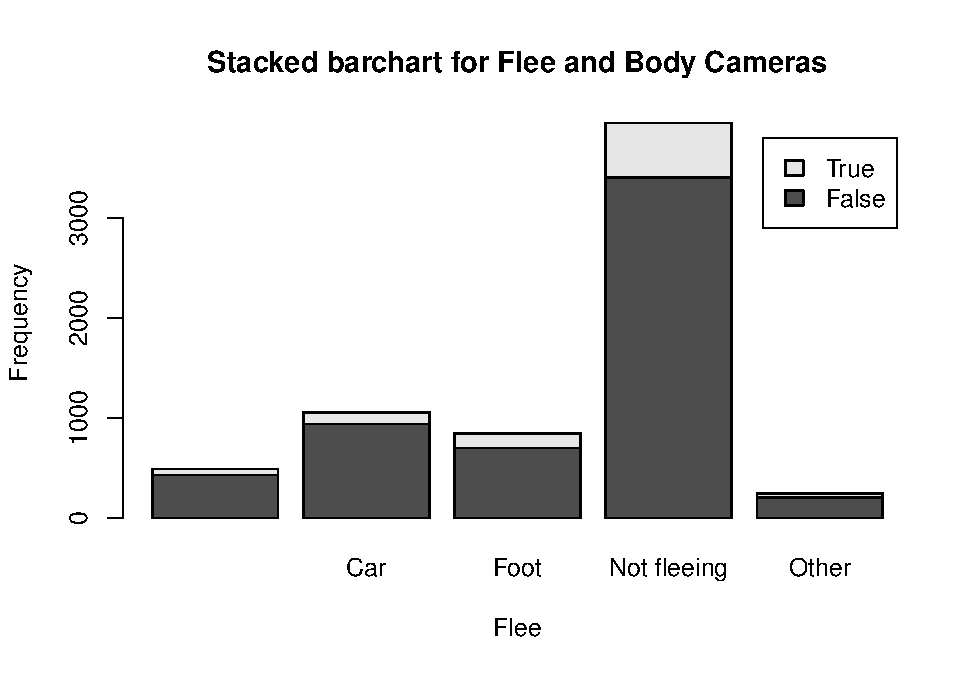
\includegraphics{Assignments_files/figure-latex/unnamed-chunk-26-1.pdf}

\textbf{For all of the categories in ``flee'', the majority of police
officers did not have a body camera. It appears that the largest
proportion of incidents with a body camera are in the ``Not fleeing''
category however, the ``Not fleeing'' category has the most
observations. Based on this plot it is hard to determine whether or not
the victim was actually fleeing because there is no video evidence of
the incident.}

\begin{enumerate}
\def\labelenumi{\alph{enumi}.}
\setcounter{enumi}{1}
\tightlist
\item
  Describe the relationship between age and race by using a boxplot.
  What can you conclude from this relationship?
\end{enumerate}

\emph{Hint 1: The categories along the x-axis are the race categories
and the height along the y-axis is age.}

\emph{Hint 2: Also, if you are unsure about the syntax for boxplot, run
?boxplot in R and see some examples at the bottom of the documentation.
This is usually a good way to look up the syntax of R code. You can also
Google it.}

\textbf{Your answer here.}

\#Extra credit (10 points)

\begin{enumerate}
\def\labelenumi{\alph{enumi}.}
\tightlist
\item
  What does this code tell us?
\end{enumerate}

\begin{Shaded}
\begin{Highlighting}[]
\NormalTok{mydates }\OtherTok{\textless{}{-}} \FunctionTok{as.Date}\NormalTok{(dat}\SpecialCharTok{$}\NormalTok{date)}
\FunctionTok{head}\NormalTok{(mydates)}
\NormalTok{(mydates[}\FunctionTok{length}\NormalTok{(mydates)] }\SpecialCharTok{{-}}\NormalTok{ mydates[}\DecValTok{1}\NormalTok{])}
\end{Highlighting}
\end{Shaded}

\textbf{This code tells us the dates of all of the incidents and how
long the data was collected for by showing the time difference.}

\begin{enumerate}
\def\labelenumi{\alph{enumi}.}
\setcounter{enumi}{1}
\tightlist
\item
  On Friday, a new report was published that was described as follows by
  The Guardian: ``More than half of US police killings are mislabelled
  or not reported, study finds.'' Without reading this article now (due
  to limited time), why do you think police killings might be
  mislabelled or underreported?
\end{enumerate}

\textbf{Police killings might be mislabelled or underreported because
there is no documentation of the shootings since the majority of
officers involved do not have a body camera to record the incident. We
have to rely on the police accounts of the incidents which could be
biased since the police do not want to show that they were in the
wrong.There is also no national system to report all police shootings to
which is confirmed by the way that the data was collected for the
Washington Post dataset.}

\begin{enumerate}
\def\labelenumi{\alph{enumi}.}
\setcounter{enumi}{2}
\tightlist
\item
  Regarding missing values in problem 4, do you see any? If so, do you
  think that's all that's missing from the data?
\end{enumerate}

\textbf{There is missing data for the variable ``Flee''.There are two
columns in the ``flee'' variable that could count under missing data.
The first column which is actually missing values and the last column
which is ``other''. The ``other'' category is not explained so we do not
know what that is reporting. There could potentially be more missing
data since the majority of incidents do not have video documentation so
the police officers could have lied about the fleeing nature of the
victim. The category for body cameras could also have missing values if
some police officers did not report whether or not they had a body
camera on or they lied.}

\[\\[2in]\]

\hypertarget{assignment-3}{%
\section{Assignment 3}\label{assignment-3}}

This assignment is due on Canvas on Wednesday 10/27/2021 before class,
at 10:15 am. Include the name of anyone with whom you collaborated at
the top of the assignment.

Submit your responses as either an HTML file or a PDF file on Canvas.
Also, please upload it to your website.

Save the file (found on Canvas) crime\_simple.txt to the same folder as
this file (your Rmd file for Assignment 3).

Load the data.

\begin{Shaded}
\begin{Highlighting}[]
\FunctionTok{library}\NormalTok{(readr)}
\FunctionTok{library}\NormalTok{(knitr)}
\NormalTok{dat.crime }\OtherTok{\textless{}{-}} \FunctionTok{read\_delim}\NormalTok{(}\StringTok{"crime\_simple.txt"}\NormalTok{, }\AttributeTok{delim =} \StringTok{"}\SpecialCharTok{\textbackslash{}t}\StringTok{"}\NormalTok{)}
\end{Highlighting}
\end{Shaded}

\begin{verbatim}
## Rows: 47 Columns: 14
\end{verbatim}

\begin{verbatim}
## -- Column specification --------------------------------------------------------
## Delimiter: "\t"
## dbl (14): R, Age, S, Ed, Ex0, Ex1, LF, M, N, NW, U1, U2, W, X
\end{verbatim}

\begin{verbatim}
## 
## i Use `spec()` to retrieve the full column specification for this data.
## i Specify the column types or set `show_col_types = FALSE` to quiet this message.
\end{verbatim}

This is a dataset from a textbook by Brian S. Everitt about crime in the
US in 1960. The data originate from the Uniform Crime Report of the FBI
and other government sources. The data for 47 states of the USA are
given.

Here is the codebook:

R: Crime rate: \# of offenses reported to police per million population

Age: The number of males of age 14-24 per 1000 population

S: Indicator variable for Southern states (0 = No, 1 = Yes)

Ed: Mean of years of schooling x 10 for persons of age 25 or older

Ex0: 1960 per capita expenditure on police by state and local government

Ex1: 1959 per capita expenditure on police by state and local government

LF: Labor force participation rate per 1000 civilian urban males age
14-24

M: The number of males per 1000 females

N: State population size in hundred thousands

NW: The number of non-whites per 1000 population

U1: Unemployment rate of urban males per 1000 of age 14-24

U2: Unemployment rate of urban males per 1000 of age 35-39

W: Median value of transferable goods and assets or family income in
tens of \$

X: The number of families per 1000 earning below 1/2 the median income

We are interested in checking whether the reported crime rate (\# of
offenses reported to police per million population) and the average
education (mean number of years of schooling for persons of age 25 or
older) are related.

\begin{enumerate}
\def\labelenumi{\arabic{enumi}.}
\tightlist
\item
  How many observations are there in the dataset? To what does each
  observation correspond?
\end{enumerate}

\begin{Shaded}
\begin{Highlighting}[]
\FunctionTok{dim}\NormalTok{(dat.crime)}
\end{Highlighting}
\end{Shaded}

\begin{verbatim}
## [1] 47 14
\end{verbatim}

\textbf{There are 47 observations in the dataset. Each observation
corresponds to one state since the data includes information from 47 out
of the 50 states. }

\begin{enumerate}
\def\labelenumi{\arabic{enumi}.}
\setcounter{enumi}{1}
\tightlist
\item
  Draw a scatterplot of the two variables. Calculate the correlation
  between the two variables. Can you come up with an explanation for
  this relationship?
\end{enumerate}

\begin{Shaded}
\begin{Highlighting}[]
\FunctionTok{plot}\NormalTok{(dat.crime}\SpecialCharTok{$}\NormalTok{R, dat.crime}\SpecialCharTok{$}\NormalTok{Ed,  }\AttributeTok{main=}\StringTok{"Relationship between Reported Crime Rate and Average Education"}\NormalTok{,}
    \AttributeTok{xlab=}\StringTok{"Number of Offenses reported per 1 million Population"}\NormalTok{, }\AttributeTok{ylab=}\StringTok{"Years of Schooling x10"}\NormalTok{)}
\end{Highlighting}
\end{Shaded}

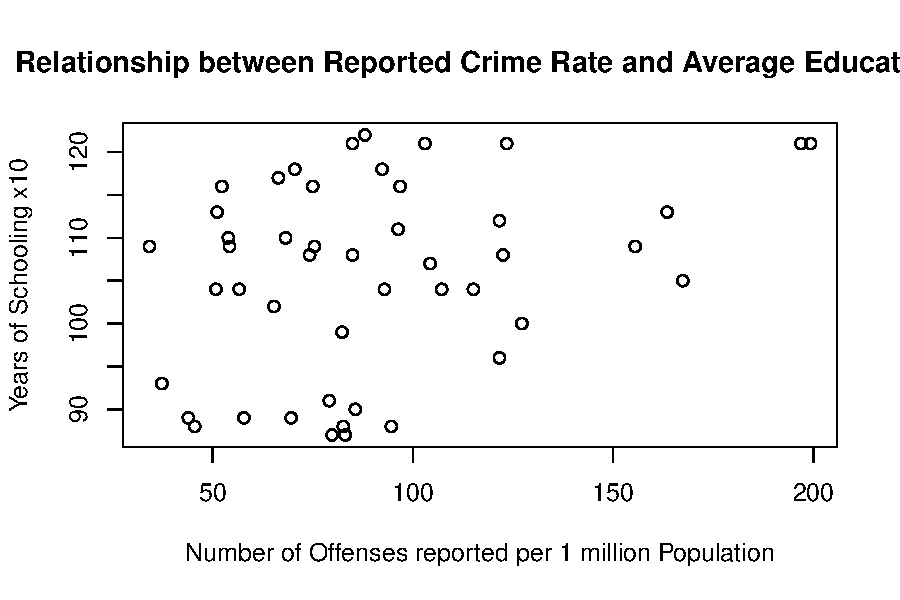
\includegraphics{Assignments_files/figure-latex/unnamed-chunk-31-1.pdf}

\begin{Shaded}
\begin{Highlighting}[]
\FunctionTok{cor}\NormalTok{(dat.crime}\SpecialCharTok{$}\NormalTok{R, dat.crime}\SpecialCharTok{$}\NormalTok{Ed)}
\end{Highlighting}
\end{Shaded}

\begin{verbatim}
## [1] 0.3228349
\end{verbatim}

\textbf{When looking at the scatter plot, the two variables do not
appear to be related as all the points are scattered and spread out. The
reported crime rate and average education have a correlation of
0.3228349 which suggest that the two variables have a slight positive
correlation. This would mean that as the number of reported offenses
increases, the average years of schooling increases. Crime rates and
education could have a positive correlation because states with a larger
population had more citizens with more years of schooling and also more
crimes.There is a possibility that people with more years of schooling
were more likely to report crimes to the police.}

\begin{enumerate}
\def\labelenumi{\arabic{enumi}.}
\setcounter{enumi}{2}
\tightlist
\item
  Regress reported crime rate (y) on average education (x) and call this
  linear model \texttt{crime.lm} and write the summary of the regression
  by using this code, which makes it look a little nicer
  \texttt{\{r,\ eval=FALSE\}\ kable(summary(crime.lm)\$coef,\ digits\ =\ 2)}.
\end{enumerate}

\begin{Shaded}
\begin{Highlighting}[]
\NormalTok{crime.lm }\OtherTok{\textless{}{-}} \FunctionTok{lm}\NormalTok{(}\AttributeTok{formula =}\NormalTok{ R }\SpecialCharTok{\textasciitilde{}}\NormalTok{ Ed, }\AttributeTok{data =}\NormalTok{ dat.crime)}

\FunctionTok{kable}\NormalTok{(}\FunctionTok{summary}\NormalTok{(crime.lm)}\SpecialCharTok{$}\NormalTok{coef, }\AttributeTok{digits =} \DecValTok{2}\NormalTok{)}
\end{Highlighting}
\end{Shaded}

\begin{longtable}[]{@{}lrrrr@{}}
\toprule
& Estimate & Std. Error & t value &
Pr(\textgreater\textbar t\textbar) \\
\midrule
\endhead
(Intercept) & -27.40 & 51.81 & -0.53 & 0.60 \\
Ed & 1.12 & 0.49 & 2.29 & 0.03 \\
\bottomrule
\end{longtable}

\begin{enumerate}
\def\labelenumi{\arabic{enumi}.}
\setcounter{enumi}{3}
\tightlist
\item
  Are the four assumptions of linear regression satisfied? To answer
  this, draw the relevant plots. (Write a maximum of one sentence per
  assumption.)
\end{enumerate}

\begin{Shaded}
\begin{Highlighting}[]
\CommentTok{\#for linearity assumption (looks good)}

\FunctionTok{plot}\NormalTok{(dat.crime}\SpecialCharTok{$}\NormalTok{Ed, crime.lm}\SpecialCharTok{$}\NormalTok{residuals, }\AttributeTok{ylim=}\FunctionTok{c}\NormalTok{(}\SpecialCharTok{{-}}\DecValTok{15}\NormalTok{,}\DecValTok{15}\NormalTok{), }\AttributeTok{main=}\StringTok{"Residuals vs. Education"}\NormalTok{, }\AttributeTok{xlab=}\StringTok{"Average Education"}\NormalTok{, }\AttributeTok{ylab=}\StringTok{"Residuals"}\NormalTok{)}
\FunctionTok{abline}\NormalTok{(}\AttributeTok{h =} \DecValTok{0}\NormalTok{, }\AttributeTok{lty=}\StringTok{"dashed"}\NormalTok{)}
\end{Highlighting}
\end{Shaded}

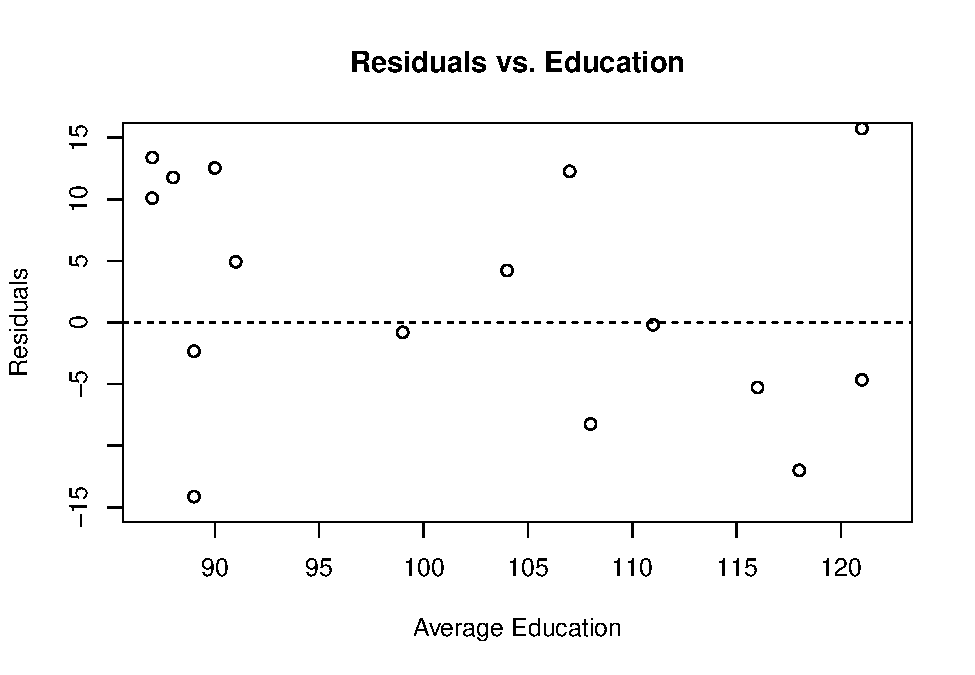
\includegraphics{Assignments_files/figure-latex/unnamed-chunk-33-1.pdf}

\begin{Shaded}
\begin{Highlighting}[]
\FunctionTok{plot}\NormalTok{(crime.lm, }\AttributeTok{which=}\DecValTok{1}\NormalTok{)}
\end{Highlighting}
\end{Shaded}

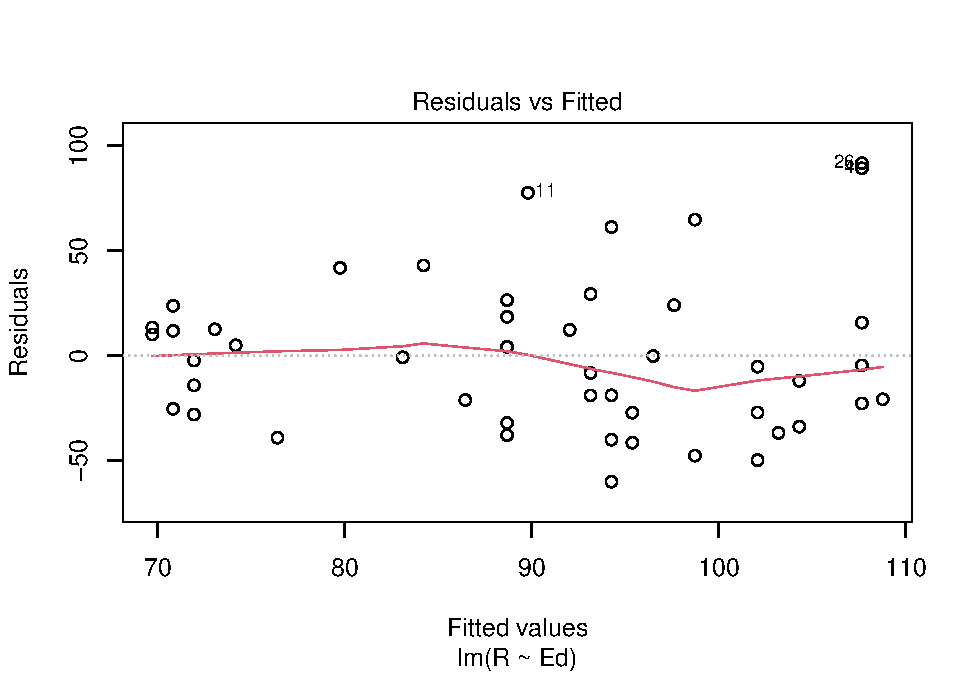
\includegraphics{Assignments_files/figure-latex/unnamed-chunk-33-2.pdf}

\begin{Shaded}
\begin{Highlighting}[]
\CommentTok{\#For Independence Assumption}

\FunctionTok{plot}\NormalTok{(dat.crime}\SpecialCharTok{$}\NormalTok{Ed, crime.lm}\SpecialCharTok{$}\NormalTok{residuals, }\AttributeTok{ylim=}\FunctionTok{c}\NormalTok{(}\SpecialCharTok{{-}}\DecValTok{15}\NormalTok{,}\DecValTok{15}\NormalTok{), }\AttributeTok{main=}\StringTok{"Residuals vs. Education"}\NormalTok{, }\AttributeTok{xlab=}\StringTok{"Average Education"}\NormalTok{, }\AttributeTok{ylab=}\StringTok{"Residuals"}\NormalTok{)}
\FunctionTok{abline}\NormalTok{(}\AttributeTok{h =} \DecValTok{0}\NormalTok{, }\AttributeTok{lty=}\StringTok{"dashed"}\NormalTok{)}
\end{Highlighting}
\end{Shaded}

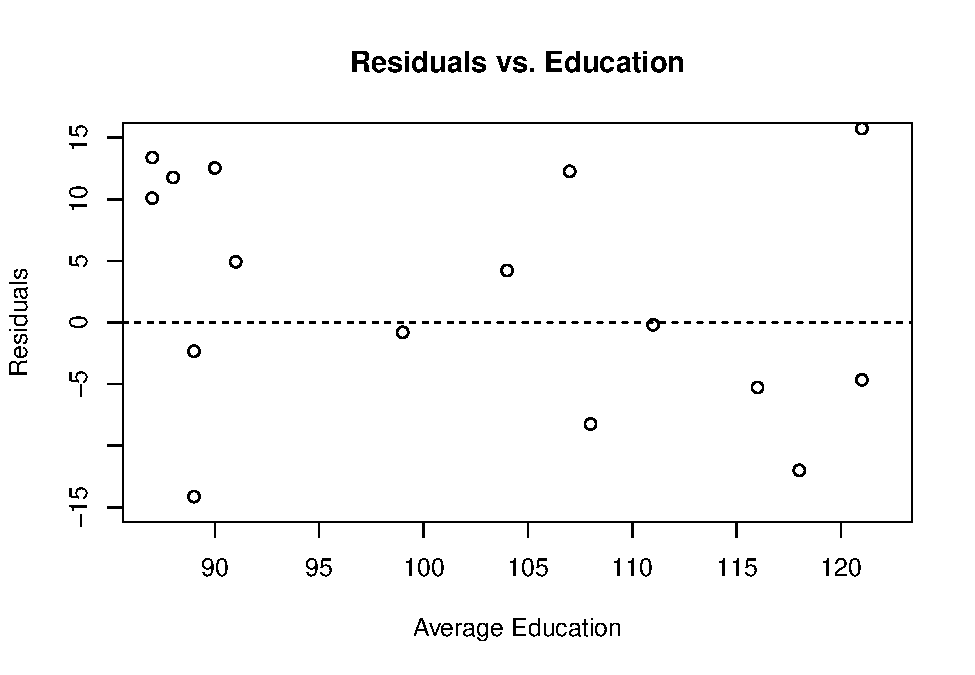
\includegraphics{Assignments_files/figure-latex/unnamed-chunk-33-3.pdf}

\begin{Shaded}
\begin{Highlighting}[]
\CommentTok{\#For Homoscedasticity Assumption}

\FunctionTok{plot}\NormalTok{(crime.lm, }\AttributeTok{which=}\DecValTok{3}\NormalTok{)}
\end{Highlighting}
\end{Shaded}

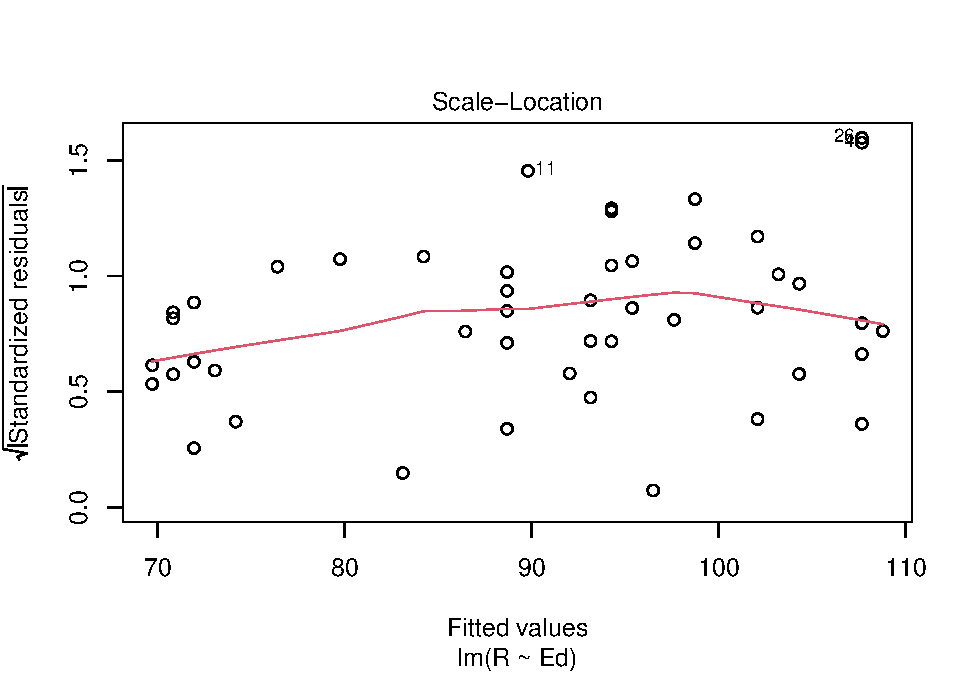
\includegraphics{Assignments_files/figure-latex/unnamed-chunk-33-4.pdf}

\begin{Shaded}
\begin{Highlighting}[]
\CommentTok{\#For Normal Population}

\FunctionTok{plot}\NormalTok{(crime.lm, }\AttributeTok{which=}\DecValTok{5}\NormalTok{)}
\end{Highlighting}
\end{Shaded}

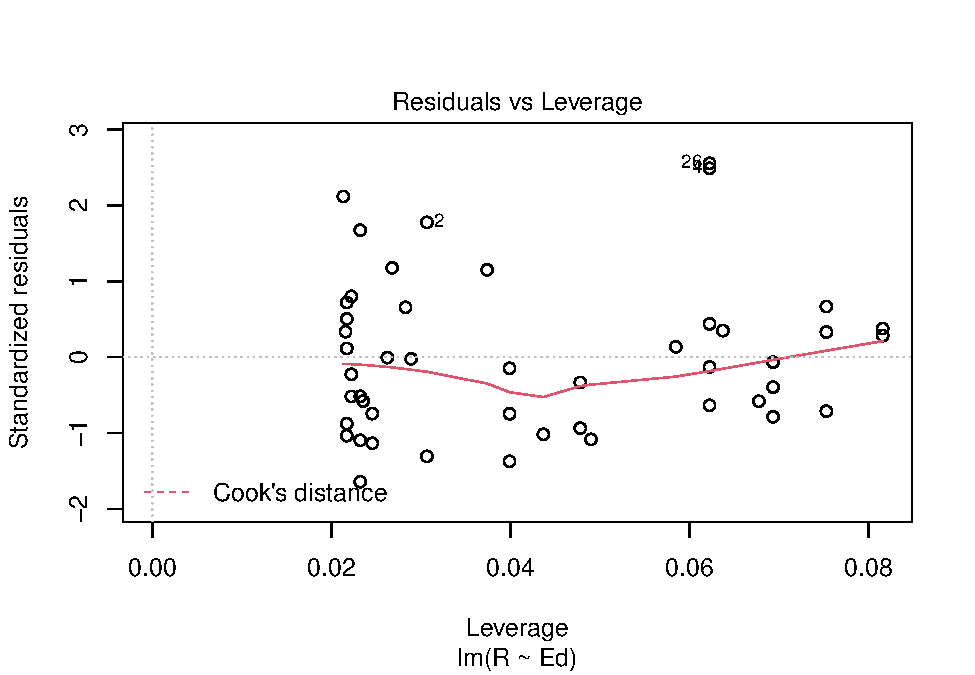
\includegraphics{Assignments_files/figure-latex/unnamed-chunk-33-5.pdf}

\begin{Shaded}
\begin{Highlighting}[]
\FunctionTok{plot}\NormalTok{(crime.lm, }\AttributeTok{which=}\DecValTok{2}\NormalTok{)}
\end{Highlighting}
\end{Shaded}

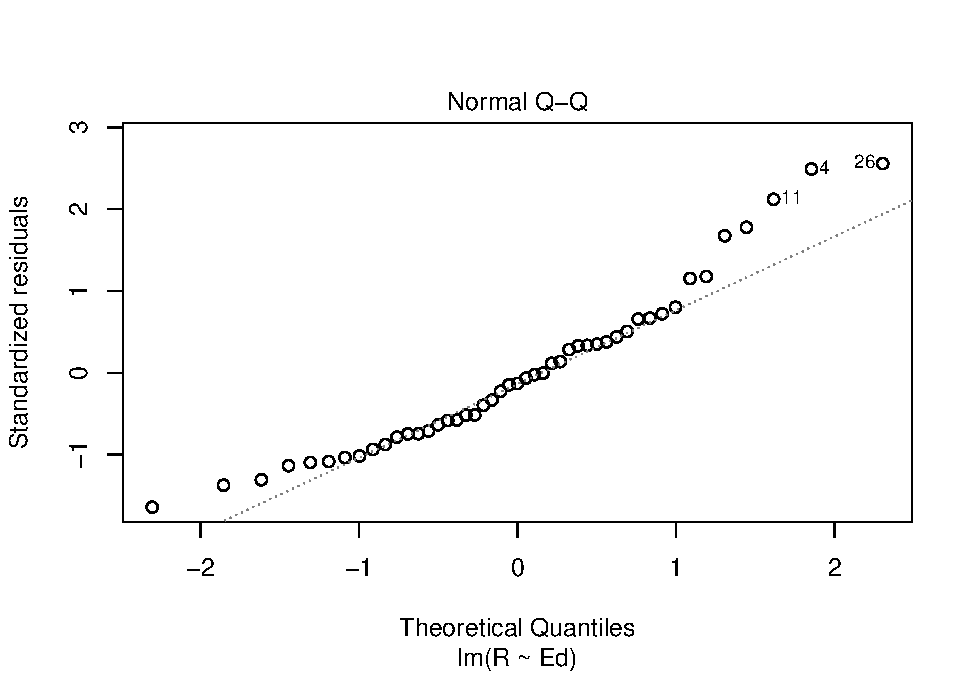
\includegraphics{Assignments_files/figure-latex/unnamed-chunk-33-6.pdf}

\textbf{For the linearity assumption, the ``Residuals vs.~fitted'' plot
has a red line that is quite straight which would mean that there is
equal variance across the range of the fitted values, so the linearity
assumption is satisfied. For the independence assumption, the
``Residuals vs Education'' plot there does not appear to be any patterns
that would indicate variable dependence and the data is not a time
series so this assumption is satisfied. For the homoscedasticity
assumption, the ``Scale-location'' plot shows a rather flat line which
would mean there is constant variance among the data which means the
homoscedasticity assumption is satisfied. For the normal population
assumption, the ``residuals vs leverage'' plot does not show any
outliers and the QQ plot shows that most points fall in line however,
the right tail is light. }

\begin{enumerate}
\def\labelenumi{\arabic{enumi}.}
\setcounter{enumi}{4}
\tightlist
\item
  Is the relationship between reported crime and average education
  statistically significant? Report the estimated coefficient of the
  slope, the standard error, and the p-value. What does it mean for the
  relationship to be statistically significant?
\end{enumerate}

\textbf{The relationship between reported crime and average education is
slightly statistically significant because the p-value is less than the
significance level. The estimated coefficient is 1.1161 which means that
for every 1 year increase in education, the crime rate goes up by
1.1161. The standard error is 0.4878 which means that the crime rate can
vary by 0.4878. The p-value is 0.0269 and it is slightly significant
because it has one asterisk. When a relationship is statistically
significant then the null hypothesis can be rejected. This means that
the relationship between the variables is not likely due to chance or
luck. }

\begin{enumerate}
\def\labelenumi{\arabic{enumi}.}
\setcounter{enumi}{5}
\tightlist
\item
  How are reported crime and average education related? In other words,
  for every unit increase in average education, how does reported crime
  rate change (per million) per state?
\end{enumerate}

\textbf{When average education increases by 1 year, the reported crime
rate increases by 1.1161 units. }

\begin{enumerate}
\def\labelenumi{\arabic{enumi}.}
\setcounter{enumi}{6}
\tightlist
\item
  Can you conclude that if individuals were to receive more education,
  then crime will be reported more often? Why or why not?
\end{enumerate}

\textbf{The conclusion that more education will lead to more reported
crimes cannot be made because correlation does not imply causation.
There are other factors involved in the reported crime rate such as
population, age and unemployment. }

\[\\[2in]\]

\hypertarget{exam-2}{%
\section{Exam 2}\label{exam-2}}

\hypertarget{data-description}{%
\subsection{Data description:}\label{data-description}}

This dataset provides (simulated) data about 200 police departments in
one year. It contains information about the funding received by the
department as well as incidents of police brutality. Suppose this
dataset (sim.data.csv) was collected by researchers to answer this
question: \textbf{``Does having more funding in a police department lead
to fewer incidents of police brutality?''}

\hypertarget{codebook}{%
\subsection{Codebook:}\label{codebook}}

\begin{itemize}
\tightlist
\item
  funds: How much funding the police department received in that year in
  millions of dollars.
\item
  po.brut: How many incidents of police brutality were reported by the
  department that year.
\item
  po.dept.code: Police department code
\end{itemize}

\hypertarget{problem-1-eda}{%
\subsubsection{Problem 1: EDA}\label{problem-1-eda}}

Describe the dataset and variables. Perform exploratory data analysis
for the two variables of interest: funds and po.brut.

\begin{Shaded}
\begin{Highlighting}[]
\NormalTok{dat }\OtherTok{\textless{}{-}} \FunctionTok{read.csv}\NormalTok{(}\AttributeTok{file =} \StringTok{\textquotesingle{}sim.data.csv\textquotesingle{}}\NormalTok{)}

\FunctionTok{head}\NormalTok{(dat)}
\end{Highlighting}
\end{Shaded}

\begin{verbatim}
##   po.dept.code funds po.brut
## 1            1  48.1      23
## 2            2  81.4      10
## 3            3  41.8      25
## 4            4  61.7      19
## 5            5  86.4       8
## 6            6  51.6      22
\end{verbatim}

\begin{Shaded}
\begin{Highlighting}[]
\FunctionTok{dim}\NormalTok{(dat)}
\end{Highlighting}
\end{Shaded}

\begin{verbatim}
## [1] 200   3
\end{verbatim}

\begin{Shaded}
\begin{Highlighting}[]
\FunctionTok{par}\NormalTok{(}\AttributeTok{mfrow=}\FunctionTok{c}\NormalTok{(}\DecValTok{2}\NormalTok{,}\DecValTok{1}\NormalTok{))}

\FunctionTok{hist}\NormalTok{(dat}\SpecialCharTok{$}\NormalTok{funds, }\AttributeTok{main=} \StringTok{"Distribution of Funds for Police Departments"}\NormalTok{, }\AttributeTok{xlab=} \StringTok{"Amount of funds (Millions of dollars)"}\NormalTok{, }\AttributeTok{ylab=} \StringTok{"Frequency"}\NormalTok{, }\AttributeTok{xlim =} \FunctionTok{c}\NormalTok{(}\DecValTok{0}\NormalTok{,}\DecValTok{100}\NormalTok{), }\AttributeTok{ylim=} \FunctionTok{c}\NormalTok{(}\DecValTok{0}\NormalTok{,}\DecValTok{100}\NormalTok{), }\AttributeTok{col=}\StringTok{"blue"}\NormalTok{)}

\FunctionTok{hist}\NormalTok{(dat}\SpecialCharTok{$}\NormalTok{po.brut, }\AttributeTok{main=} \StringTok{"Distribution of Incidents of Police Brutality  for Police Departments"}\NormalTok{, }\AttributeTok{xlab=} \StringTok{"Incidents of Policy Brutality"}\NormalTok{, }\AttributeTok{ylab=} \StringTok{"Frequency"}\NormalTok{, }\AttributeTok{xlim =} \FunctionTok{c}\NormalTok{(}\DecValTok{0}\NormalTok{,}\DecValTok{100}\NormalTok{), }\AttributeTok{ylim=} \FunctionTok{c}\NormalTok{(}\DecValTok{0}\NormalTok{,}\DecValTok{100}\NormalTok{), }\AttributeTok{col=}\StringTok{"red"}\NormalTok{)}
\end{Highlighting}
\end{Shaded}

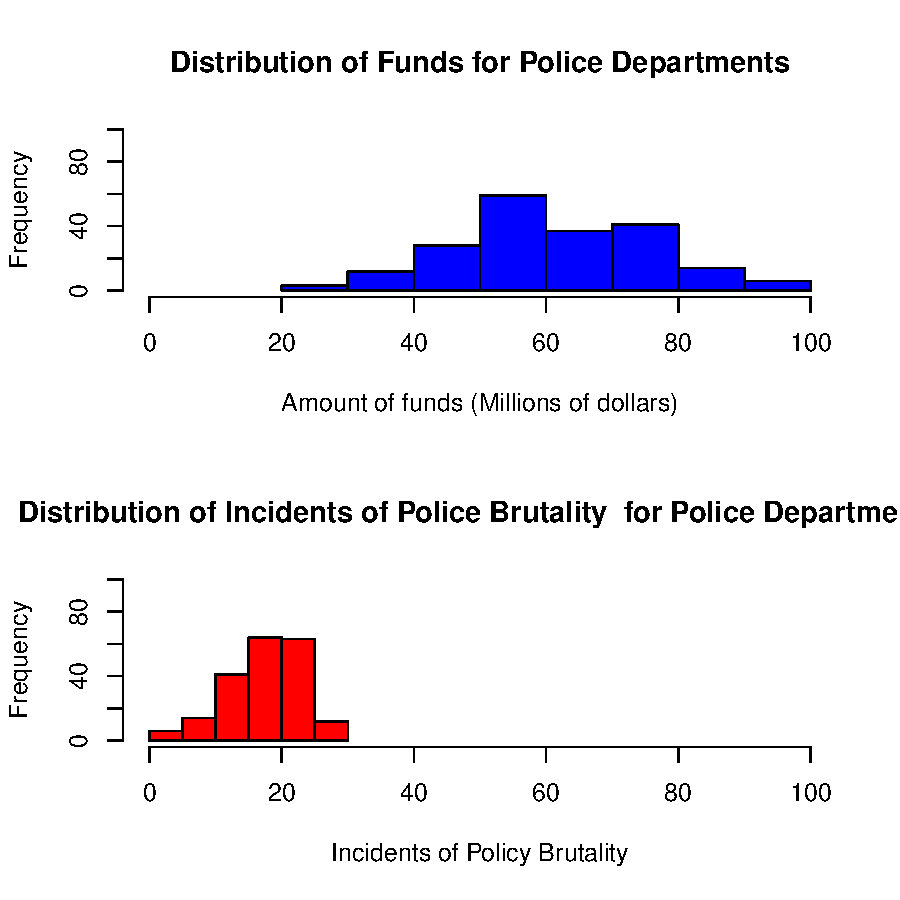
\includegraphics{Assignments_files/figure-latex/unnamed-chunk-34-1.pdf}

\textbf{The dataset contains 200 observations. Each observation
corresponds to a police department. There are three columns that
correspond to the three variables of police department code, funding
that each department received and incidents of police brutality for each
department.The distribution for funds appears to be almost normal with a
slight skew to the right. The distribution for incidents of police
brutality appears to have a slight left skew with the most frequent
number of incidents being around 20. }

\hypertarget{problem-2-linear-regression}{%
\subsubsection{Problem 2: Linear
regression}\label{problem-2-linear-regression}}

\begin{enumerate}
\def\labelenumi{\alph{enumi}.}
\tightlist
\item
  Perform a simple linear regression to answer the question of interest.
  To do this, name your linear model ``reg.output'' and write the
  summary of the regression by using ``summary(reg.output)''.
\end{enumerate}

\begin{Shaded}
\begin{Highlighting}[]
\NormalTok{reg.output }\OtherTok{\textless{}{-}} \FunctionTok{lm}\NormalTok{(}\AttributeTok{formula =}\NormalTok{ po.brut }\SpecialCharTok{\textasciitilde{}}\NormalTok{ funds, }\AttributeTok{data =}\NormalTok{ dat)}

\FunctionTok{summary}\NormalTok{(reg.output)}
\end{Highlighting}
\end{Shaded}

\begin{verbatim}
## 
## Call:
## lm(formula = po.brut ~ funds, data = dat)
## 
## Residuals:
##     Min      1Q  Median      3Q     Max 
## -3.9433 -0.2233  0.2544  0.5952  1.1803 
## 
## Coefficients:
##              Estimate Std. Error t value Pr(>|t|)    
## (Intercept) 40.543069   0.282503  143.51   <2e-16 ***
## funds       -0.367099   0.004496  -81.64   <2e-16 ***
## ---
## Signif. codes:  0 '***' 0.001 '**' 0.01 '*' 0.05 '.' 0.1 ' ' 1
## 
## Residual standard error: 0.9464 on 198 degrees of freedom
## Multiple R-squared:  0.9712, Adjusted R-squared:  0.971 
## F-statistic:  6666 on 1 and 198 DF,  p-value: < 2.2e-16
\end{verbatim}

\begin{enumerate}
\def\labelenumi{\alph{enumi}.}
\setcounter{enumi}{1}
\tightlist
\item
  Report the estimated coefficient, standard error, and p-value of the
  slope. Is the relationship between funds and incidents statistically
  significant? Explain.
\end{enumerate}

\textbf{The estimated coefficient is -0.367099 which means that a one
million dollar increase in amount of funds is associated with a decrease
of -0.367099 incidents of police brutality. The standard error is
0.004496 which means that the change in incidents of police brutality
can vary by 0.004496. The p-value is \textless{} 2.2e-16 and it is
statistically significant because there are three asterisks. The p-value
is less than the alpha value of 0.05 which means that the relationship
between funds and incidents is statistically significant and the null
hypothesis can be rejected which means that the observed relationship is
not due to chance. }

\begin{enumerate}
\def\labelenumi{\alph{enumi}.}
\setcounter{enumi}{2}
\tightlist
\item
  Draw a scatterplot of po.brut (y-axis) and funds (x-axis). Right below
  your plot command, use abline to draw the fitted regression line, like
  this:
\end{enumerate}

\begin{Shaded}
\begin{Highlighting}[]
\FunctionTok{plot}\NormalTok{(dat}\SpecialCharTok{$}\NormalTok{funds, dat}\SpecialCharTok{$}\NormalTok{po.brut,  }\AttributeTok{main=}\StringTok{"Relationship between Funds Recieved and Incidents of Police Brutality"}\NormalTok{, }\AttributeTok{xlab=}\StringTok{"Funds Recieved (Millions of Dollars)"}\NormalTok{, }\AttributeTok{ylab=}\StringTok{"Incidents of Police Brutality"}\NormalTok{)}
\FunctionTok{abline}\NormalTok{(reg.output, }\AttributeTok{col =} \StringTok{"red"}\NormalTok{, }\AttributeTok{lwd=}\DecValTok{2}\NormalTok{)}
\end{Highlighting}
\end{Shaded}

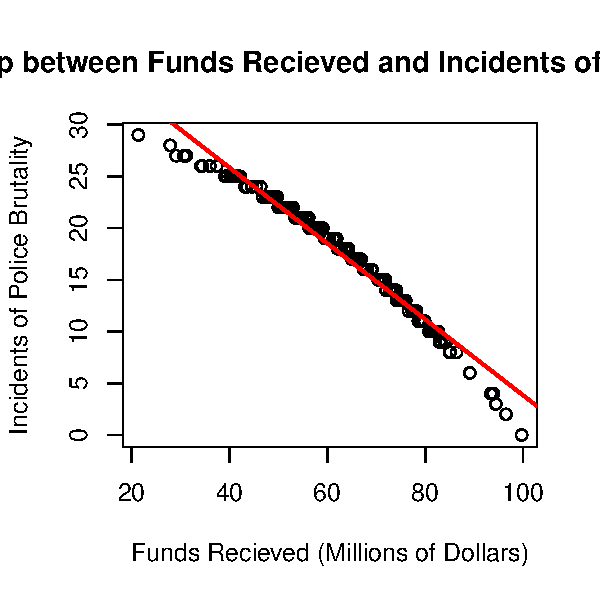
\includegraphics{Assignments_files/figure-latex/unnamed-chunk-36-1.pdf}

\begin{Shaded}
\begin{Highlighting}[]
\CommentTok{\#for linearity assumption}

\FunctionTok{plot}\NormalTok{(reg.output, }\AttributeTok{which=}\DecValTok{1}\NormalTok{)}
\end{Highlighting}
\end{Shaded}

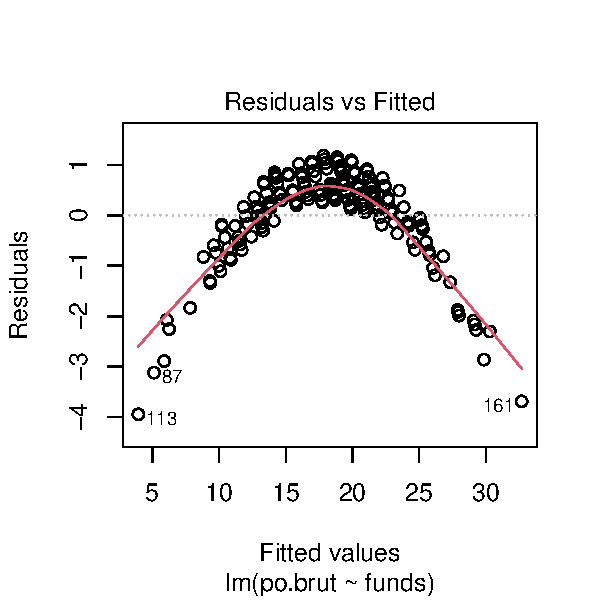
\includegraphics{Assignments_files/figure-latex/unnamed-chunk-36-2.pdf}

\begin{Shaded}
\begin{Highlighting}[]
\CommentTok{\#For Independence Assumption}

\FunctionTok{plot}\NormalTok{(dat}\SpecialCharTok{$}\NormalTok{funds, reg.output}\SpecialCharTok{$}\NormalTok{residuals, }\AttributeTok{ylim=}\FunctionTok{c}\NormalTok{(}\SpecialCharTok{{-}}\DecValTok{15}\NormalTok{,}\DecValTok{15}\NormalTok{), }\AttributeTok{main=}\StringTok{"Residuals vs. Funds"}\NormalTok{, }\AttributeTok{xlab=}\StringTok{"Funds Recieved (Millions of Dollars)"}\NormalTok{, }\AttributeTok{ylab=}\StringTok{"Residuals"}\NormalTok{)}
\FunctionTok{abline}\NormalTok{(}\AttributeTok{h =} \DecValTok{0}\NormalTok{, }\AttributeTok{lty=}\StringTok{"dashed"}\NormalTok{)}
\end{Highlighting}
\end{Shaded}

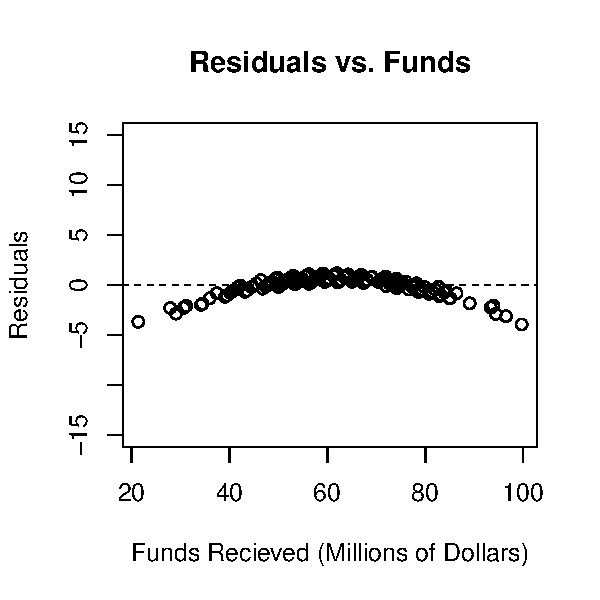
\includegraphics{Assignments_files/figure-latex/unnamed-chunk-36-3.pdf}

\begin{Shaded}
\begin{Highlighting}[]
\CommentTok{\#For Homoscedasticity Assumption}

\FunctionTok{plot}\NormalTok{(reg.output, }\AttributeTok{which=}\DecValTok{3}\NormalTok{)}
\end{Highlighting}
\end{Shaded}

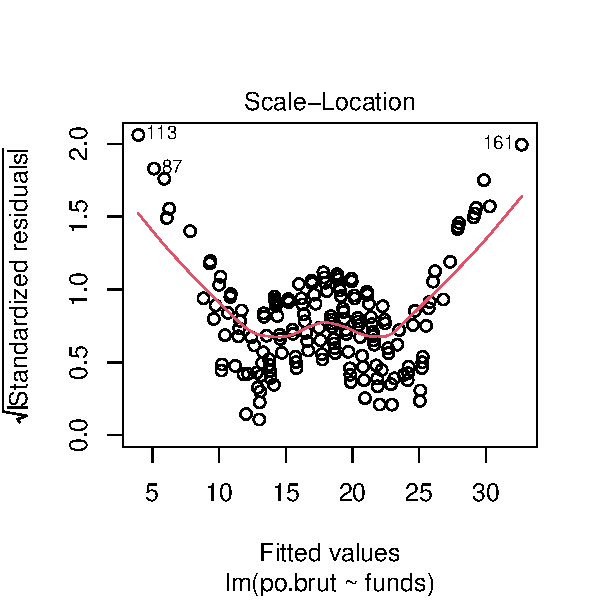
\includegraphics{Assignments_files/figure-latex/unnamed-chunk-36-4.pdf}

\begin{Shaded}
\begin{Highlighting}[]
\CommentTok{\#For Normal Population}

\FunctionTok{plot}\NormalTok{(reg.output, }\AttributeTok{which=}\DecValTok{5}\NormalTok{)}
\end{Highlighting}
\end{Shaded}

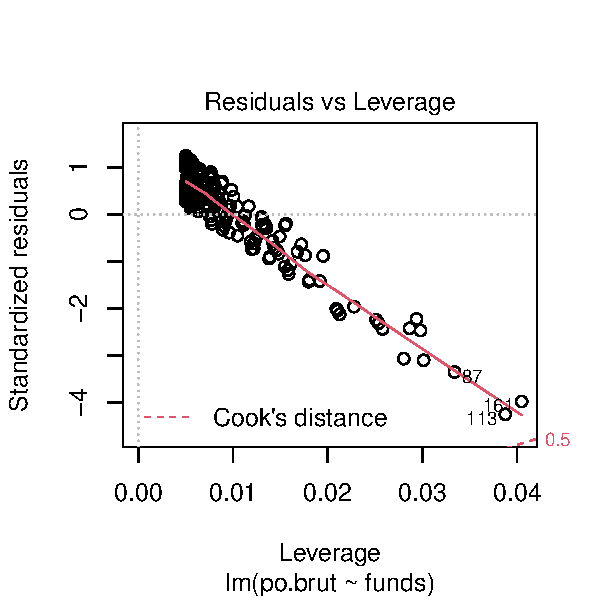
\includegraphics{Assignments_files/figure-latex/unnamed-chunk-36-5.pdf}

\begin{Shaded}
\begin{Highlighting}[]
\FunctionTok{plot}\NormalTok{(reg.output, }\AttributeTok{which=}\DecValTok{2}\NormalTok{)}
\end{Highlighting}
\end{Shaded}

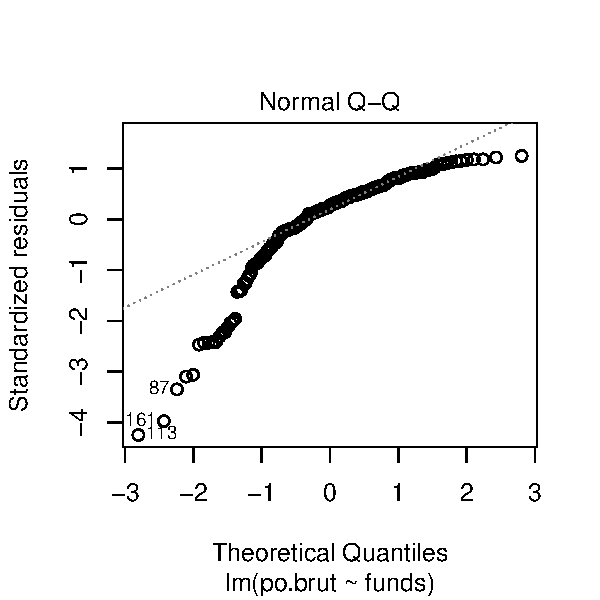
\includegraphics{Assignments_files/figure-latex/unnamed-chunk-36-6.pdf}
Does the line look like a good fit? Why or why not?

\textbf{The line looks like a good fit because most of the points fall
on the line.}

\begin{enumerate}
\def\labelenumi{\alph{enumi}.}
\setcounter{enumi}{3}
\tightlist
\item
  Are the four assumptions of linear regression satisfied? To answer
  this, draw the relevant plots. (Write a maximum of one sentence per
  assumption.) If not, what might you try to do to improve this (if you
  had more time)?
\end{enumerate}

\textbf{For the linearity assumption, on the ``Residuals vs Fitted''
plot the points follow a pattern and there is not equal variance between
them which means that linearity is not satisfied. For the independence
assumption, the dataset is not a time series since the data is collected
from 200 different police departments and the ``Residuals vs Funds''
plot does not suggest variable dependence which means the assumption is
satisfied but it is hard to tell from the plot alone. For the
homoscedasticity assumption, the scale-location plot does not show equal
variance among the points and the line is curved which does not suggest
a linear trend therefore this assumption is not satisfied. For the
normal population assumption, there does not appear to be any outliers
but the Q-Q plot shows that the points do not follow the line and
instead curve which means that the data is left skewed and not normal so
the assumption is not satisfied. To improve the data so the assumptions
are satisfied, the data can be transformed with log. The log of
incidents of police brutality can be taken to see if that makes the data
fit the model better. }

\begin{enumerate}
\def\labelenumi{\alph{enumi}.}
\setcounter{enumi}{4}
\tightlist
\item
  Answer the question of interest based on your analysis.
\end{enumerate}

\textbf{When looking at the scatterplot and linear regression summary
and plot, it appears that having more funding decreases incidents of
police brutality. However, the linear regression model is not a a good
model to make a conclusion off of because all of the assumptions tested
were not satisfied. Since the assumptions were not satisfied, the linear
regression model is not a good fit for the data.In order to come to a
clearer conclusion about the relationship between funding and incidents
of police brutality, the model needs to be transformed. }

\hypertarget{problem-3-data-ethics}{%
\subsubsection{Problem 3: Data ethics}\label{problem-3-data-ethics}}

Describe the dataset. Considering our lecture on data ethics, what
concerns do you have about the dataset? Once you perform your analysis
to answer the question of interest using this dataset, what concerns
might you have about the results?

\textbf{The dataset includes observations from 200 police departments
about funding received and incidents of police brutality in one
year.Some concerns about the data are sampling bias since we do not know
which police departments were chosen and how they were chosen. If most
of the police departments come from one area then the data is not
representative of the population and could be biased. We also do not
know who the researchers were and who funded their study which could be
another concern for bias. There is also a concern that the police
departments were not accurate with their report for incidents of police
brutality since that could make a police department look bad. The
results from the analysis can be misleading because there is statistical
significance and the R value and correlation are high so it appears that
there is a relationship between funding and incidents. However, when
assumptions are checked they are not satisfied which means that the
model is not a good fit so conclusions should not be made using it.}

\[\\[2in]\]

\hypertarget{assignment-4}{%
\section{Assignment 4}\label{assignment-4}}

\hypertarget{working-with-ggplot}{%
\subsection{Working with GGPlot}\label{working-with-ggplot}}

\hypertarget{data-visualization}{%
\subsubsection{Data Visualization}\label{data-visualization}}

\begin{Shaded}
\begin{Highlighting}[]
\CommentTok{\#install.packages("tidyverse")}
\FunctionTok{library}\NormalTok{(tidyverse)}
\end{Highlighting}
\end{Shaded}

\begin{verbatim}
## -- Attaching packages --------------------------------------- tidyverse 1.3.1 --
\end{verbatim}

\begin{verbatim}
## v tibble  3.1.4     v dplyr   1.0.7
## v tidyr   1.1.4     v stringr 1.4.0
## v purrr   0.3.4     v forcats 0.5.1
\end{verbatim}

\begin{verbatim}
## -- Conflicts ------------------------------------------ tidyverse_conflicts() --
## x dplyr::filter() masks stats::filter()
## x dplyr::lag()    masks stats::lag()
## x purrr::map()    masks maps::map()
\end{verbatim}

\begin{Shaded}
\begin{Highlighting}[]
\CommentTok{\#install.packages("dplyr")}
\FunctionTok{library}\NormalTok{(dplyr) }
\CommentTok{\#\textgreater{} ── Attaching packages ─────────────────────────────────────── tidyverse 1.3.0 ──}
\CommentTok{\#\textgreater{} ✔ ggplot2 3.3.2     ✔ purrr   0.3.4}
\CommentTok{\#\textgreater{} ✔ tibble  3.0.3     ✔ dplyr   1.0.2}
\CommentTok{\#\textgreater{} ✔ tidyr   1.1.2     ✔ stringr 1.4.0}
\CommentTok{\#\textgreater{} ✔ readr   1.4.0     ✔ forcats 0.5.0}
\CommentTok{\#\textgreater{} ── Conflicts ────────────────────────────────────────── tidyverse\_conflicts() ──}
\CommentTok{\#\textgreater{} ✖ dplyr::filter() masks stats::filter()}
\CommentTok{\#\textgreater{} ✖ dplyr::lag()    masks stats::lag()}
\end{Highlighting}
\end{Shaded}

Installed library tidyverse for ggplot 2

\begin{Shaded}
\begin{Highlighting}[]
\FunctionTok{ggplot}\NormalTok{(}\AttributeTok{data =}\NormalTok{ mpg) }\SpecialCharTok{+} 
  \FunctionTok{geom\_point}\NormalTok{(}\AttributeTok{mapping =} \FunctionTok{aes}\NormalTok{(}\AttributeTok{x =}\NormalTok{ displ, }\AttributeTok{y =}\NormalTok{ hwy))}
\end{Highlighting}
\end{Shaded}

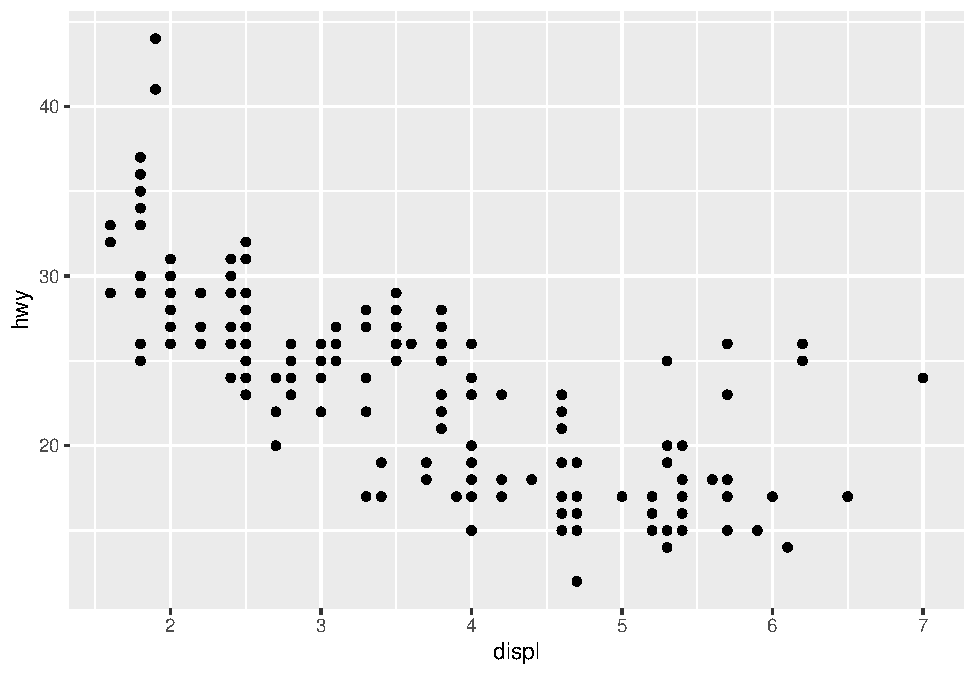
\includegraphics{Assignments_files/figure-latex/unnamed-chunk-38-1.pdf}

Creates a ggplot using mpg dataframe which comes with the ggplot
package.

\begin{Shaded}
\begin{Highlighting}[]
\FunctionTok{ggplot}\NormalTok{(}\AttributeTok{data =}\NormalTok{ mpg) }\SpecialCharTok{+} 
  \FunctionTok{geom\_point}\NormalTok{(}\AttributeTok{mapping =} \FunctionTok{aes}\NormalTok{(}\AttributeTok{x =}\NormalTok{ displ, }\AttributeTok{y =}\NormalTok{ hwy, }\AttributeTok{color =}\NormalTok{ class))}
\end{Highlighting}
\end{Shaded}

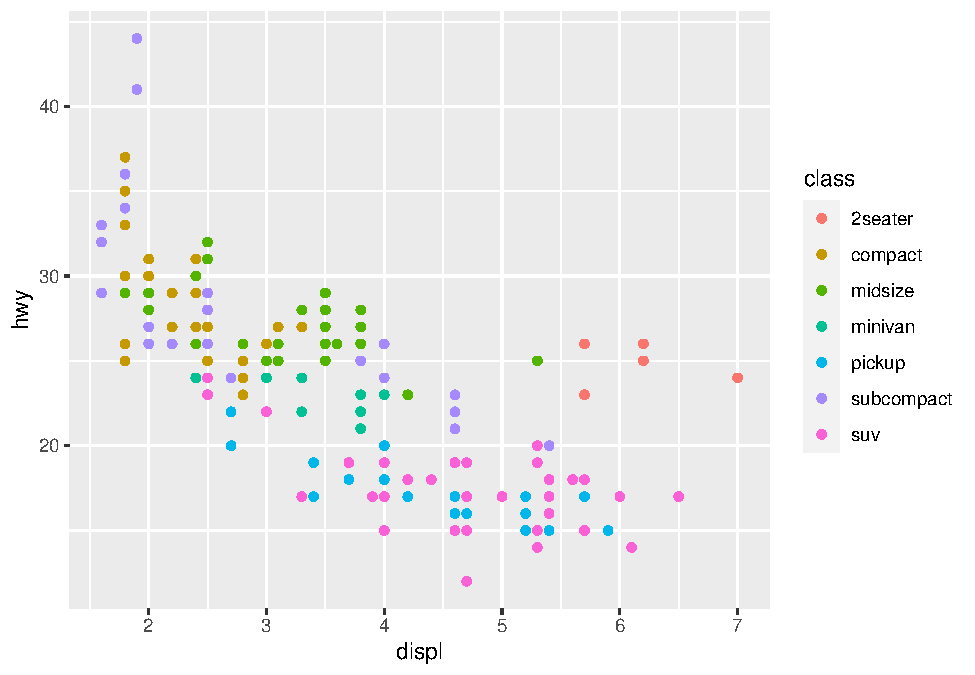
\includegraphics{Assignments_files/figure-latex/unnamed-chunk-39-1.pdf}

Using aes adds aesthetics to the plot like color and shape which can be
used to add a third variable to a two dimensional graph. In this case,
each color corresponds to a different class of car.Using size for the
variable class is not advised.

\begin{Shaded}
\begin{Highlighting}[]
\CommentTok{\# Left}
\FunctionTok{ggplot}\NormalTok{(}\AttributeTok{data =}\NormalTok{ mpg) }\SpecialCharTok{+} 
  \FunctionTok{geom\_point}\NormalTok{(}\AttributeTok{mapping =} \FunctionTok{aes}\NormalTok{(}\AttributeTok{x =}\NormalTok{ displ, }\AttributeTok{y =}\NormalTok{ hwy, }\AttributeTok{alpha =}\NormalTok{ class))}
\end{Highlighting}
\end{Shaded}

\begin{verbatim}
## Warning: Using alpha for a discrete variable is not advised.
\end{verbatim}

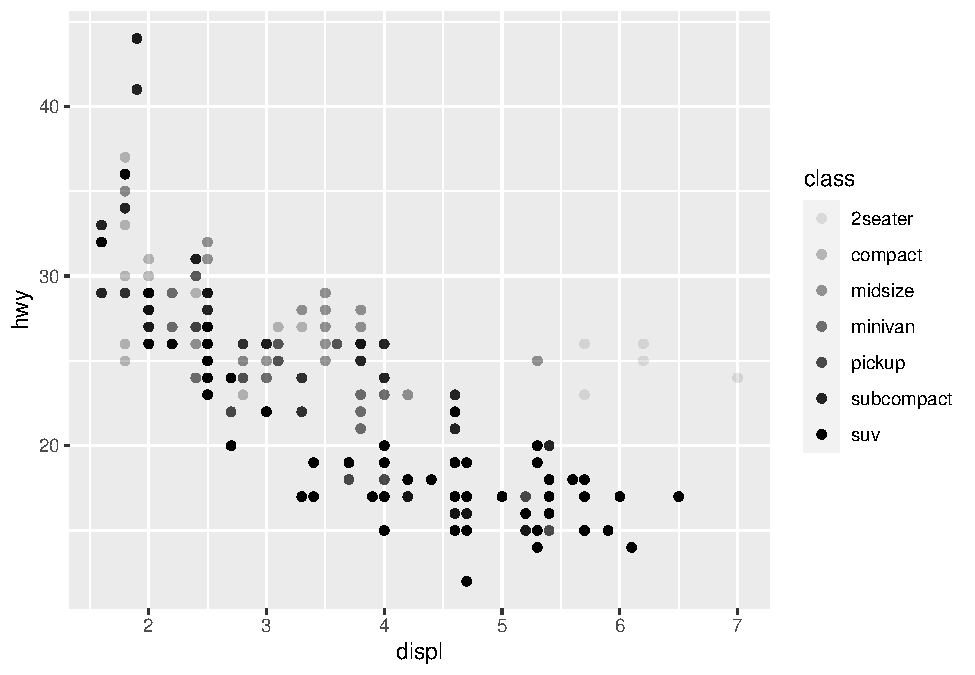
\includegraphics{Assignments_files/figure-latex/unnamed-chunk-40-1.pdf}

\begin{Shaded}
\begin{Highlighting}[]
\CommentTok{\# Right}
\FunctionTok{ggplot}\NormalTok{(}\AttributeTok{data =}\NormalTok{ mpg) }\SpecialCharTok{+} 
  \FunctionTok{geom\_point}\NormalTok{(}\AttributeTok{mapping =} \FunctionTok{aes}\NormalTok{(}\AttributeTok{x =}\NormalTok{ displ, }\AttributeTok{y =}\NormalTok{ hwy, }\AttributeTok{shape =}\NormalTok{ class))}
\end{Highlighting}
\end{Shaded}

\begin{verbatim}
## Warning: The shape palette can deal with a maximum of 6 discrete values because
## more than 6 becomes difficult to discriminate; you have 7. Consider
## specifying shapes manually if you must have them.
\end{verbatim}

\begin{verbatim}
## Warning: Removed 62 rows containing missing values (geom_point).
\end{verbatim}

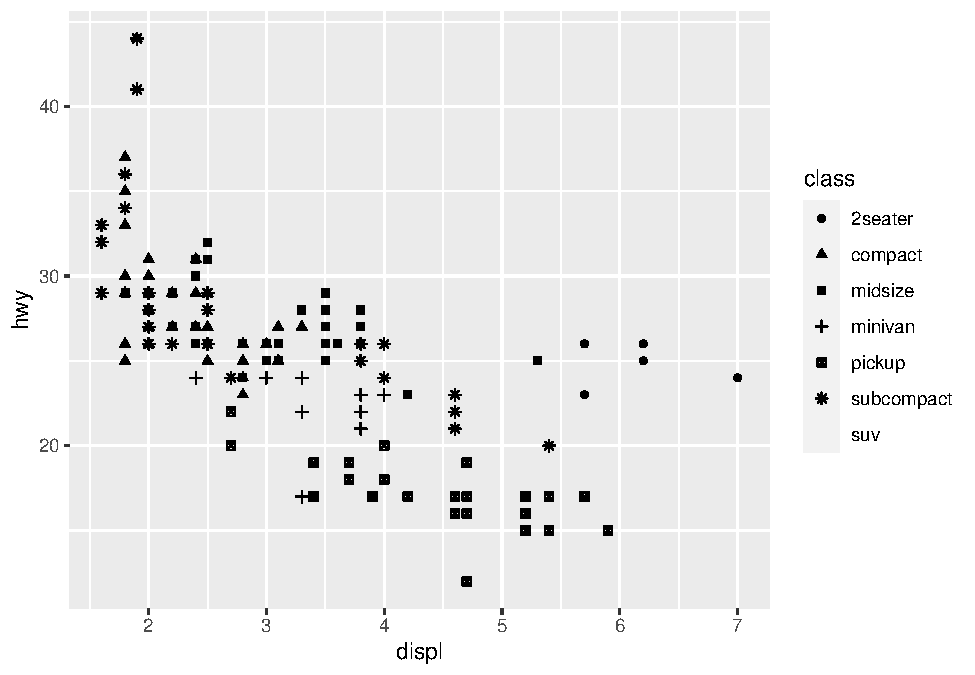
\includegraphics{Assignments_files/figure-latex/unnamed-chunk-40-2.pdf}
alpha controls the transparency of the points and shape controls the
shape of the points. Only six shapes can be used at a time. When writing
code in ggplot2 make sure the + comes at the end of the line not the
start.

\begin{Shaded}
\begin{Highlighting}[]
\FunctionTok{ggplot}\NormalTok{(}\AttributeTok{data =}\NormalTok{ mpg) }\SpecialCharTok{+} 
  \FunctionTok{geom\_point}\NormalTok{(}\AttributeTok{mapping =} \FunctionTok{aes}\NormalTok{(}\AttributeTok{x =}\NormalTok{ displ, }\AttributeTok{y =}\NormalTok{ hwy)) }\SpecialCharTok{+} 
  \FunctionTok{facet\_wrap}\NormalTok{(}\SpecialCharTok{\textasciitilde{}}\NormalTok{ class, }\AttributeTok{nrow =} \DecValTok{2}\NormalTok{)}
\end{Highlighting}
\end{Shaded}

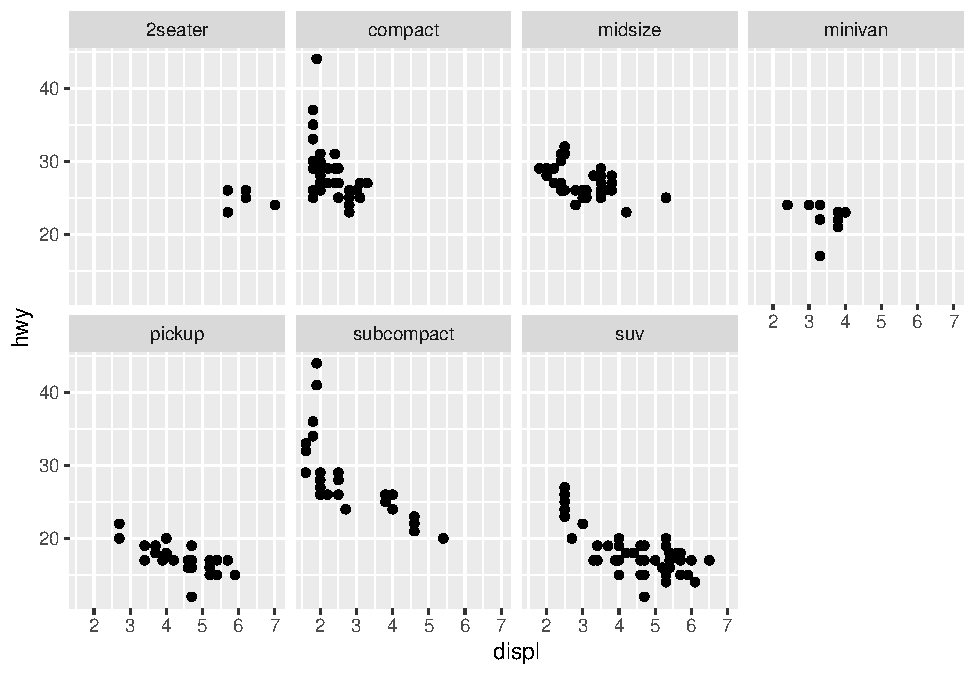
\includegraphics{Assignments_files/figure-latex/unnamed-chunk-41-1.pdf}
``facets'' split the plot into subplots that display one subset of the
data. This is useful for categorical variables.

\begin{Shaded}
\begin{Highlighting}[]
\CommentTok{\# left}
\FunctionTok{ggplot}\NormalTok{(}\AttributeTok{data =}\NormalTok{ mpg) }\SpecialCharTok{+} 
  \FunctionTok{geom\_point}\NormalTok{(}\AttributeTok{mapping =} \FunctionTok{aes}\NormalTok{(}\AttributeTok{x =}\NormalTok{ displ, }\AttributeTok{y =}\NormalTok{ hwy))}
\end{Highlighting}
\end{Shaded}

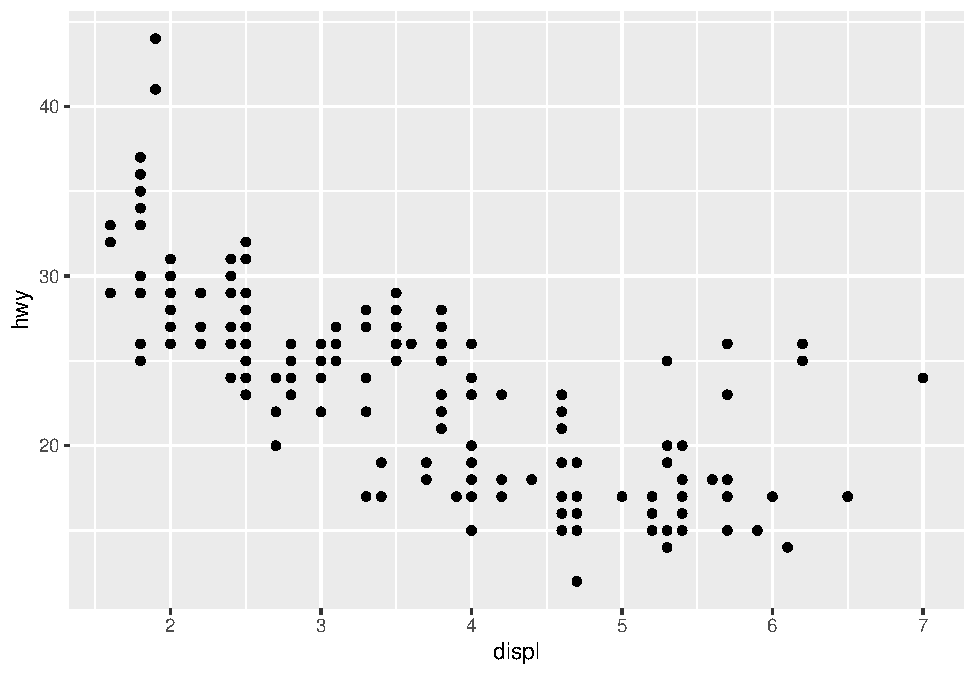
\includegraphics{Assignments_files/figure-latex/unnamed-chunk-42-1.pdf}

\begin{Shaded}
\begin{Highlighting}[]
\CommentTok{\# right}
\FunctionTok{ggplot}\NormalTok{(}\AttributeTok{data =}\NormalTok{ mpg) }\SpecialCharTok{+} 
  \FunctionTok{geom\_smooth}\NormalTok{(}\AttributeTok{mapping =} \FunctionTok{aes}\NormalTok{(}\AttributeTok{x =}\NormalTok{ displ, }\AttributeTok{y =}\NormalTok{ hwy))}
\end{Highlighting}
\end{Shaded}

\begin{verbatim}
## `geom_smooth()` using method = 'loess' and formula 'y ~ x'
\end{verbatim}

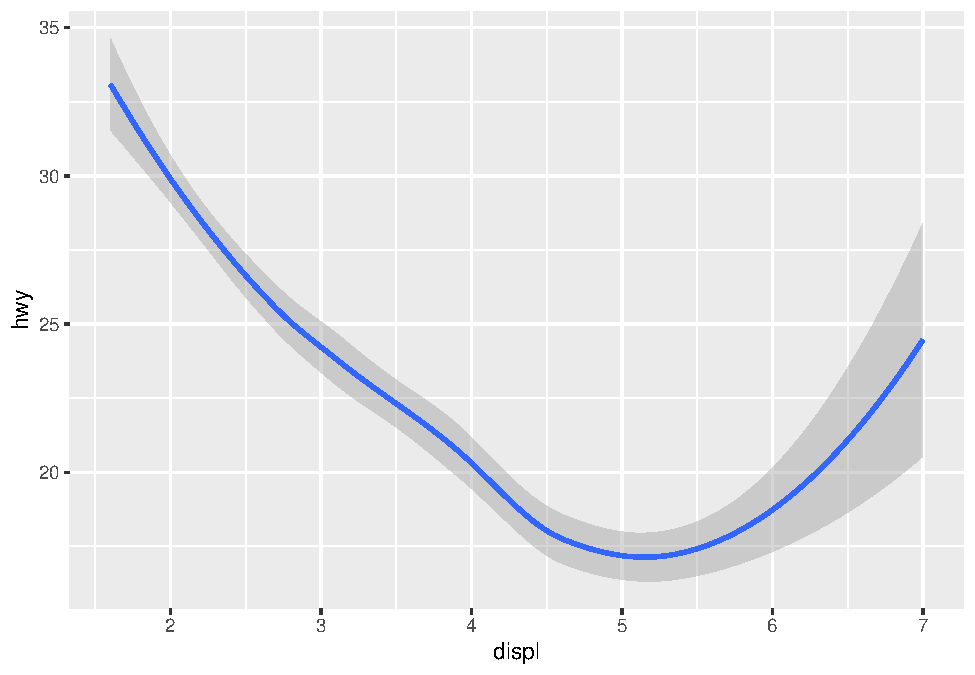
\includegraphics{Assignments_files/figure-latex/unnamed-chunk-42-2.pdf}
Using geom changes the geometrical object of the plot. geoms can be used
for box plots, scatter plots, bar plots, line chats and etc.

\begin{Shaded}
\begin{Highlighting}[]
\FunctionTok{ggplot}\NormalTok{(}\AttributeTok{data =}\NormalTok{ mpg) }\SpecialCharTok{+}
  \FunctionTok{geom\_smooth}\NormalTok{(}\AttributeTok{mapping =} \FunctionTok{aes}\NormalTok{(}\AttributeTok{x =}\NormalTok{ displ, }\AttributeTok{y =}\NormalTok{ hwy))}
\end{Highlighting}
\end{Shaded}

\begin{verbatim}
## `geom_smooth()` using method = 'loess' and formula 'y ~ x'
\end{verbatim}

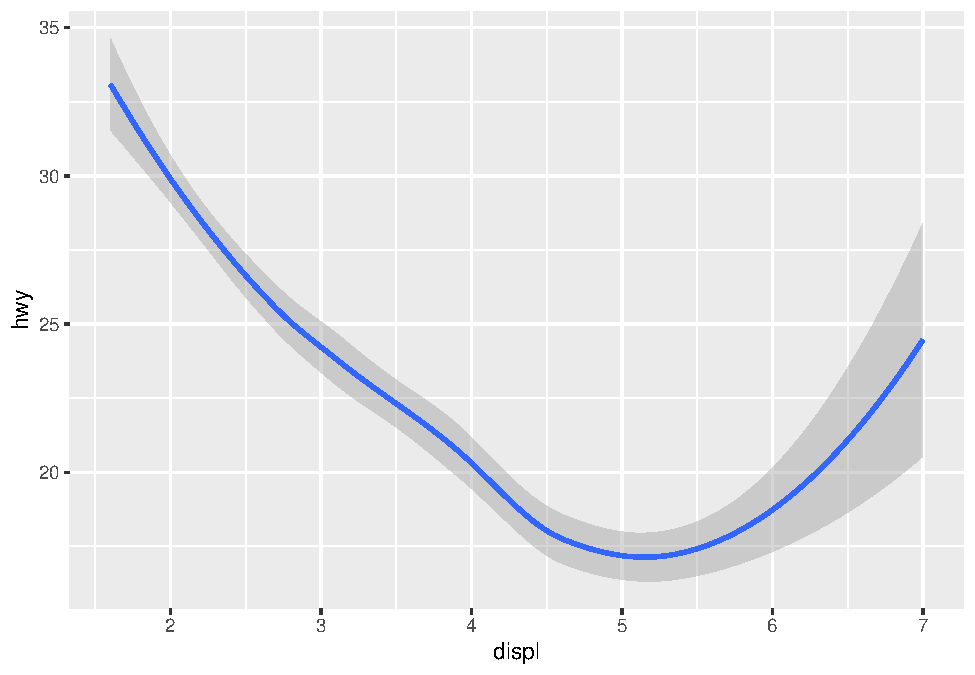
\includegraphics{Assignments_files/figure-latex/unnamed-chunk-43-1.pdf}

\begin{Shaded}
\begin{Highlighting}[]
\FunctionTok{ggplot}\NormalTok{(}\AttributeTok{data =}\NormalTok{ mpg) }\SpecialCharTok{+}
  \FunctionTok{geom\_smooth}\NormalTok{(}\AttributeTok{mapping =} \FunctionTok{aes}\NormalTok{(}\AttributeTok{x =}\NormalTok{ displ, }\AttributeTok{y =}\NormalTok{ hwy, }\AttributeTok{group =}\NormalTok{ drv))}
\end{Highlighting}
\end{Shaded}

\begin{verbatim}
## `geom_smooth()` using method = 'loess' and formula 'y ~ x'
\end{verbatim}

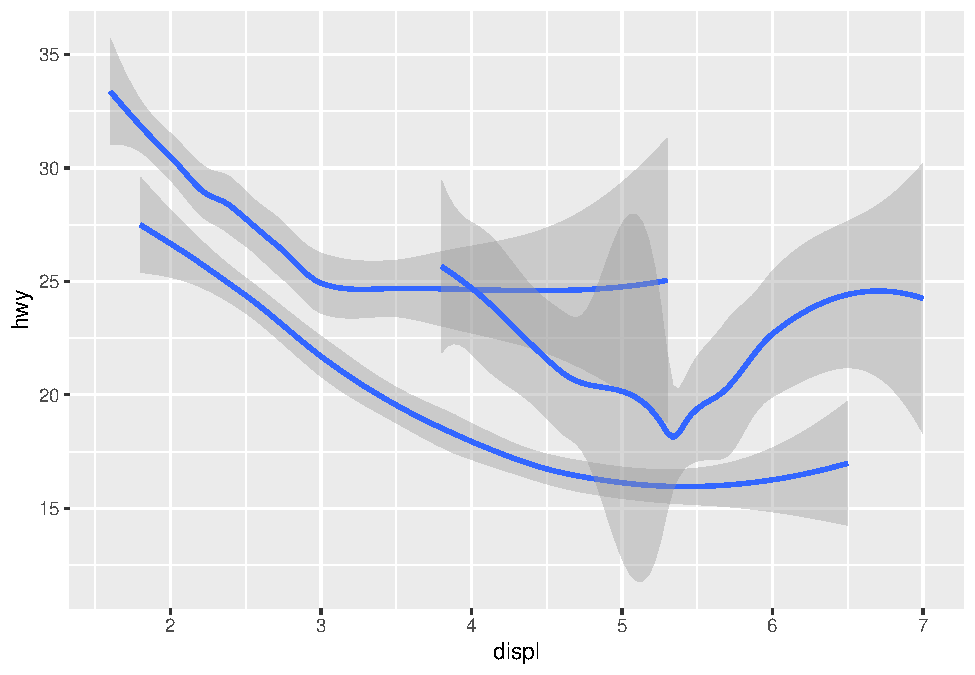
\includegraphics{Assignments_files/figure-latex/unnamed-chunk-43-2.pdf}

\begin{Shaded}
\begin{Highlighting}[]
\FunctionTok{ggplot}\NormalTok{(}\AttributeTok{data =}\NormalTok{ mpg) }\SpecialCharTok{+}
  \FunctionTok{geom\_smooth}\NormalTok{(}
    \AttributeTok{mapping =} \FunctionTok{aes}\NormalTok{(}\AttributeTok{x =}\NormalTok{ displ, }\AttributeTok{y =}\NormalTok{ hwy, }\AttributeTok{color =}\NormalTok{ drv),}
    \AttributeTok{show.legend =} \ConstantTok{FALSE}
\NormalTok{  )}
\end{Highlighting}
\end{Shaded}

\begin{verbatim}
## `geom_smooth()` using method = 'loess' and formula 'y ~ x'
\end{verbatim}

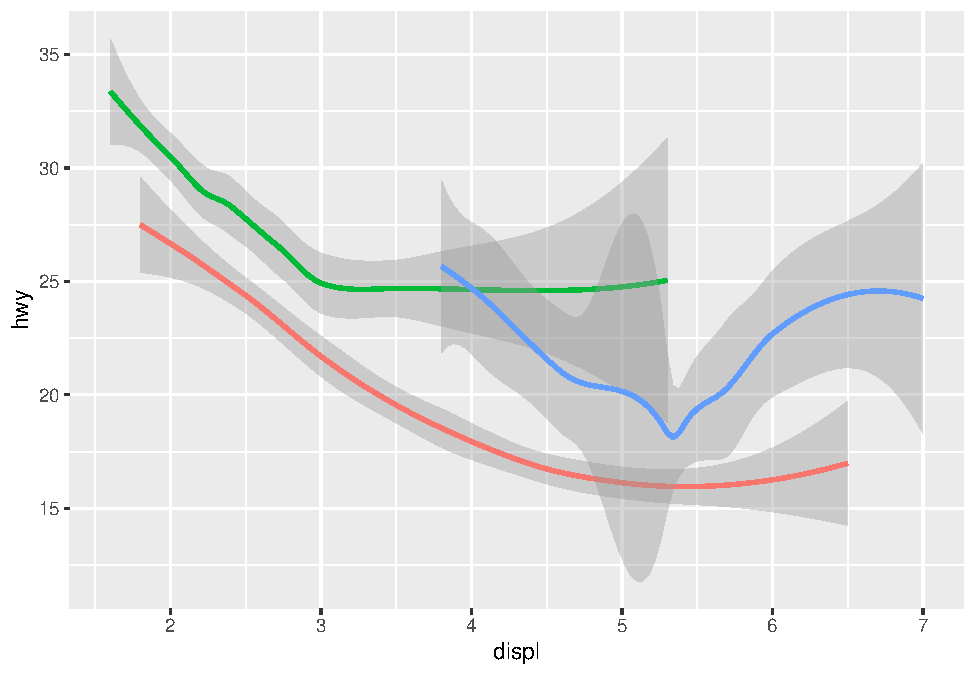
\includegraphics{Assignments_files/figure-latex/unnamed-chunk-43-3.pdf}
One geometric object can display multiple rows of data by setting the
group aesthetic to a categorical variable.

\begin{Shaded}
\begin{Highlighting}[]
\FunctionTok{ggplot}\NormalTok{(}\AttributeTok{data =}\NormalTok{ mpg) }\SpecialCharTok{+} 
  \FunctionTok{geom\_point}\NormalTok{(}\AttributeTok{mapping =} \FunctionTok{aes}\NormalTok{(}\AttributeTok{x =}\NormalTok{ displ, }\AttributeTok{y =}\NormalTok{ hwy)) }\SpecialCharTok{+}
  \FunctionTok{geom\_smooth}\NormalTok{(}\AttributeTok{mapping =} \FunctionTok{aes}\NormalTok{(}\AttributeTok{x =}\NormalTok{ displ, }\AttributeTok{y =}\NormalTok{ hwy))}
\end{Highlighting}
\end{Shaded}

\begin{verbatim}
## `geom_smooth()` using method = 'loess' and formula 'y ~ x'
\end{verbatim}

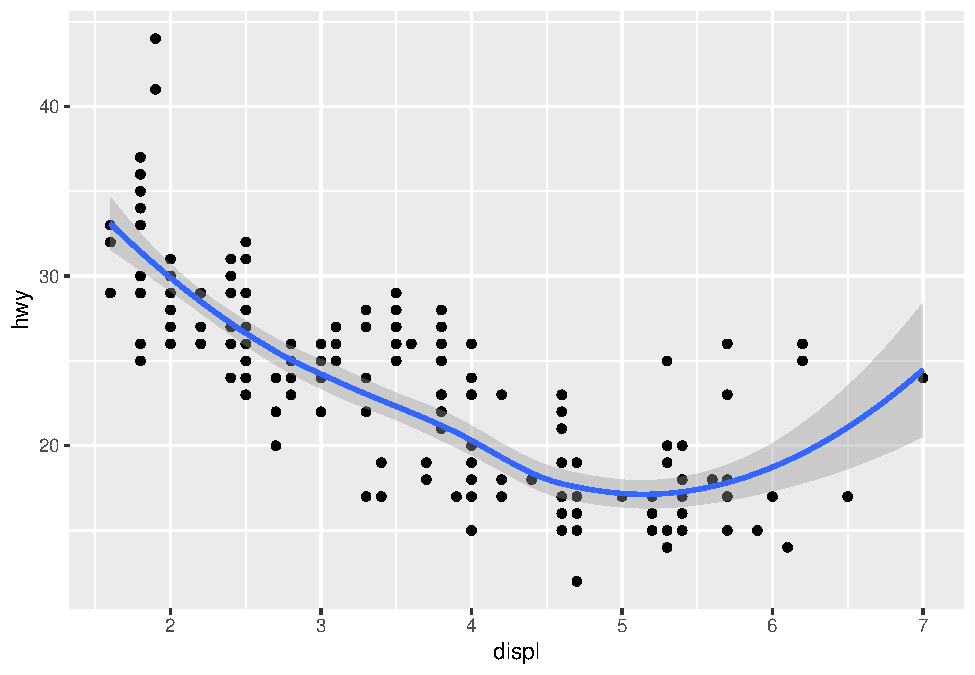
\includegraphics{Assignments_files/figure-latex/unnamed-chunk-44-1.pdf}
Plots multiple geom functions to one ggplot.

\begin{Shaded}
\begin{Highlighting}[]
\FunctionTok{ggplot}\NormalTok{(}\AttributeTok{data =}\NormalTok{ mpg, }\AttributeTok{mapping =} \FunctionTok{aes}\NormalTok{(}\AttributeTok{x =}\NormalTok{ displ, }\AttributeTok{y =}\NormalTok{ hwy)) }\SpecialCharTok{+} 
  \FunctionTok{geom\_point}\NormalTok{() }\SpecialCharTok{+} 
  \FunctionTok{geom\_smooth}\NormalTok{()}
\end{Highlighting}
\end{Shaded}

\begin{verbatim}
## `geom_smooth()` using method = 'loess' and formula 'y ~ x'
\end{verbatim}

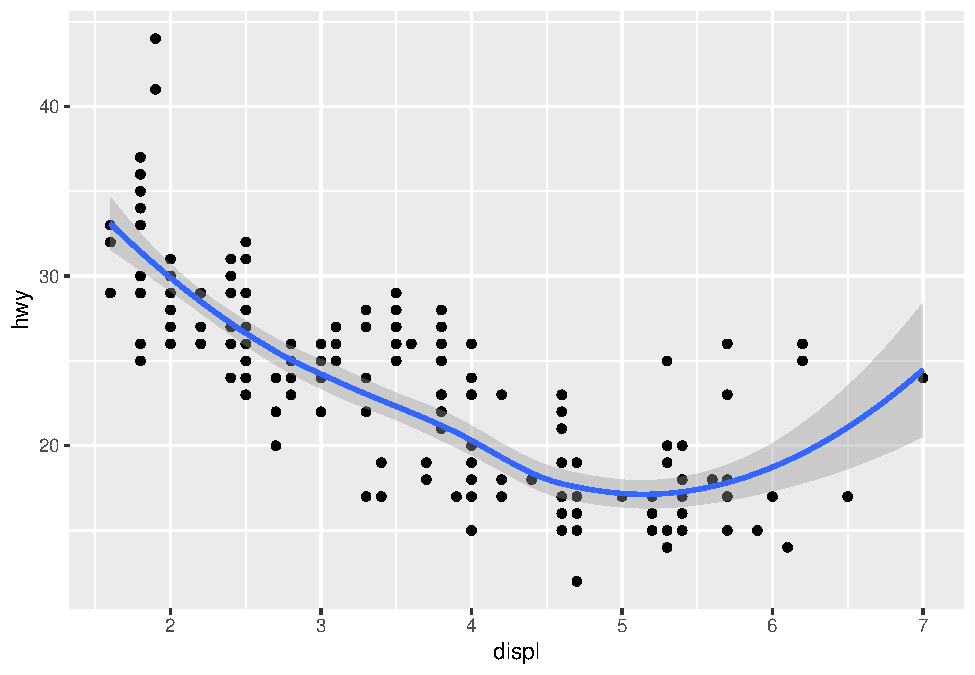
\includegraphics{Assignments_files/figure-latex/unnamed-chunk-45-1.pdf}
This code plots the same plots as above but reduces duplication in the
code.

\begin{Shaded}
\begin{Highlighting}[]
\FunctionTok{ggplot}\NormalTok{(}\AttributeTok{data =}\NormalTok{ diamonds) }\SpecialCharTok{+} 
  \FunctionTok{geom\_bar}\NormalTok{(}\AttributeTok{mapping =} \FunctionTok{aes}\NormalTok{(}\AttributeTok{x =}\NormalTok{ cut))}
\end{Highlighting}
\end{Shaded}

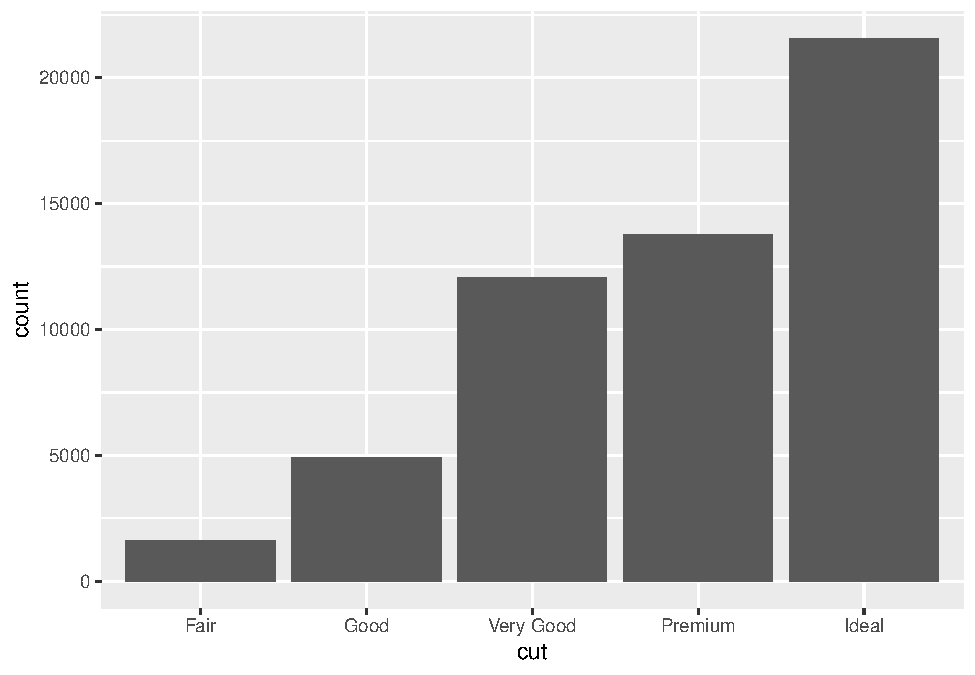
\includegraphics{Assignments_files/figure-latex/unnamed-chunk-46-1.pdf}
Creates a bar plot which creates bins for your data instead of raw data.

\begin{Shaded}
\begin{Highlighting}[]
\FunctionTok{ggplot}\NormalTok{(}\AttributeTok{data =}\NormalTok{ diamonds) }\SpecialCharTok{+} 
  \FunctionTok{stat\_summary}\NormalTok{(}
    \AttributeTok{mapping =} \FunctionTok{aes}\NormalTok{(}\AttributeTok{x =}\NormalTok{ cut, }\AttributeTok{y =}\NormalTok{ depth),}
    \AttributeTok{fun.min =}\NormalTok{ min,}
    \AttributeTok{fun.max =}\NormalTok{ max,}
    \AttributeTok{fun =}\NormalTok{ median}
\NormalTok{  )}
\end{Highlighting}
\end{Shaded}

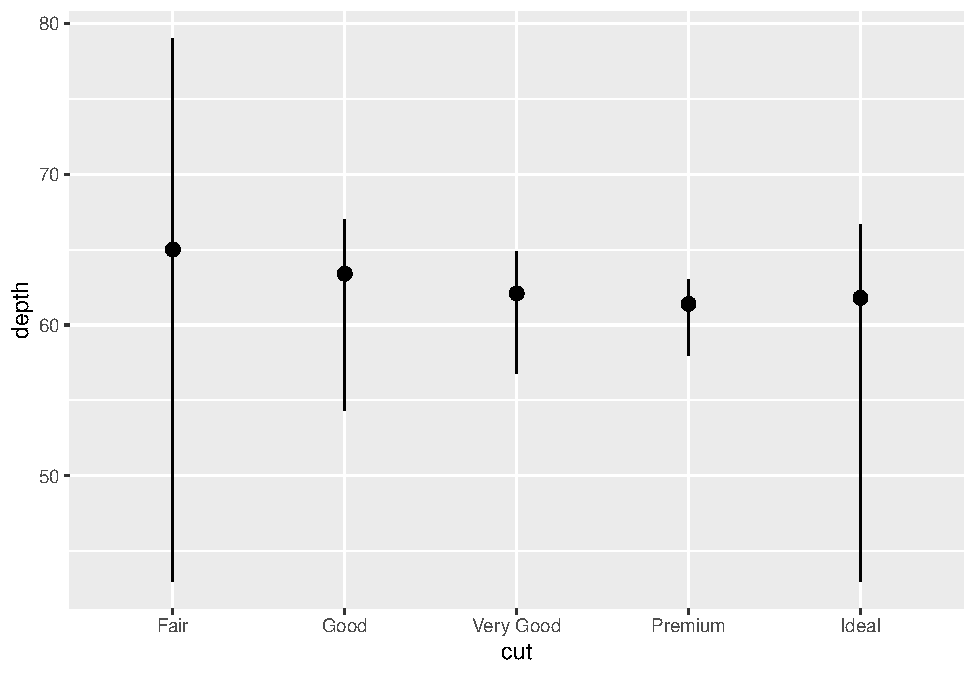
\includegraphics{Assignments_files/figure-latex/unnamed-chunk-47-1.pdf}
Plots the statistical summary for the y values.

\begin{Shaded}
\begin{Highlighting}[]
\FunctionTok{ggplot}\NormalTok{(}\AttributeTok{data =}\NormalTok{ diamonds) }\SpecialCharTok{+} 
  \FunctionTok{geom\_bar}\NormalTok{(}\AttributeTok{mapping =} \FunctionTok{aes}\NormalTok{(}\AttributeTok{x =}\NormalTok{ cut, }\AttributeTok{colour =}\NormalTok{ cut))}
\end{Highlighting}
\end{Shaded}

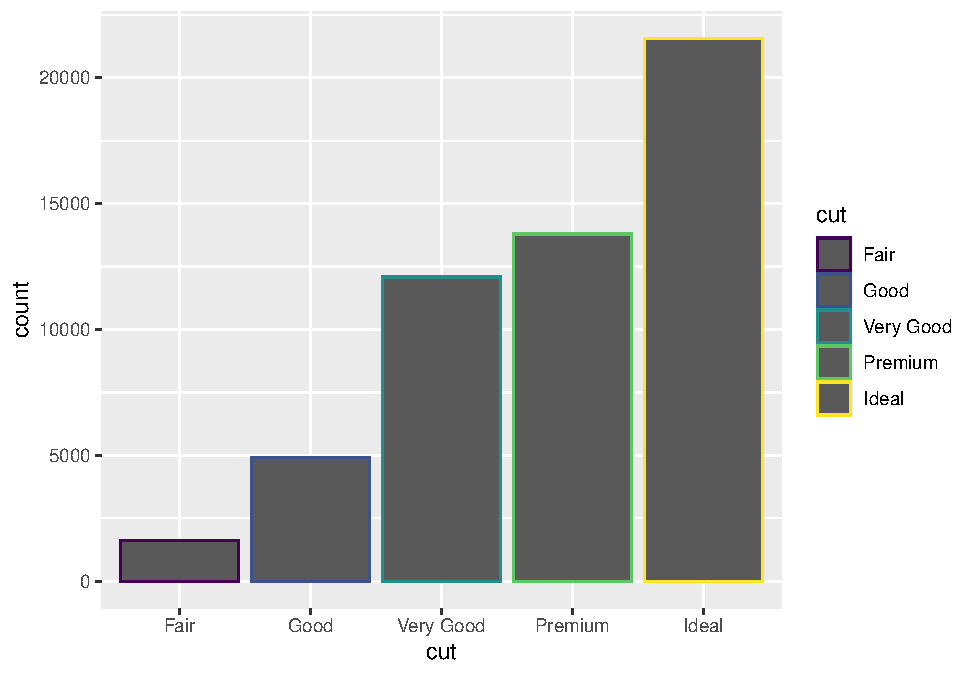
\includegraphics{Assignments_files/figure-latex/unnamed-chunk-48-1.pdf}

\begin{Shaded}
\begin{Highlighting}[]
\FunctionTok{ggplot}\NormalTok{(}\AttributeTok{data =}\NormalTok{ diamonds) }\SpecialCharTok{+} 
  \FunctionTok{geom\_bar}\NormalTok{(}\AttributeTok{mapping =} \FunctionTok{aes}\NormalTok{(}\AttributeTok{x =}\NormalTok{ cut, }\AttributeTok{fill =}\NormalTok{ cut))}
\end{Highlighting}
\end{Shaded}

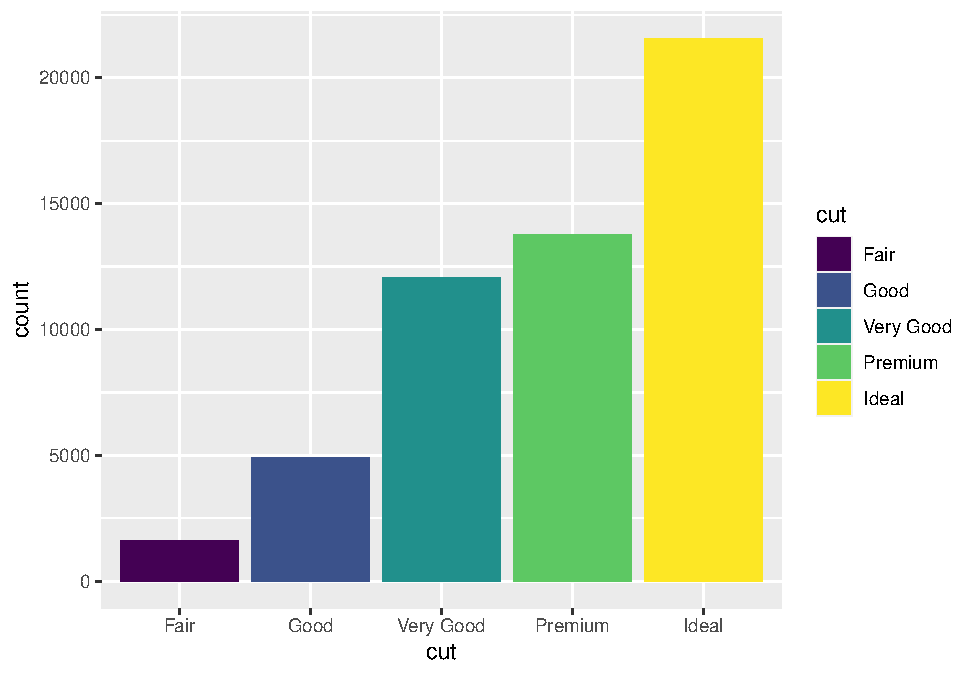
\includegraphics{Assignments_files/figure-latex/unnamed-chunk-48-2.pdf}
To change the color of the bars in a bar plot.

\begin{Shaded}
\begin{Highlighting}[]
\FunctionTok{ggplot}\NormalTok{(}\AttributeTok{data =}\NormalTok{ diamonds) }\SpecialCharTok{+} 
  \FunctionTok{geom\_bar}\NormalTok{(}\AttributeTok{mapping =} \FunctionTok{aes}\NormalTok{(}\AttributeTok{x =}\NormalTok{ cut, }\AttributeTok{fill =}\NormalTok{ clarity))}
\end{Highlighting}
\end{Shaded}

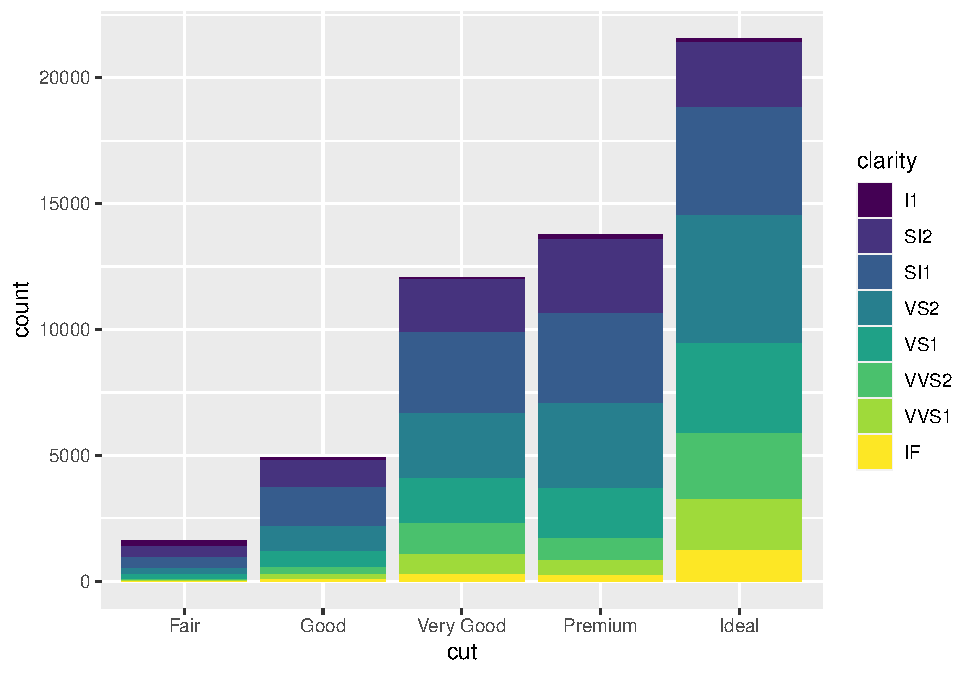
\includegraphics{Assignments_files/figure-latex/unnamed-chunk-49-1.pdf}
Changes the color in each bar to represent multiple variables.

\begin{Shaded}
\begin{Highlighting}[]
\FunctionTok{ggplot}\NormalTok{(}\AttributeTok{data =}\NormalTok{ diamonds) }\SpecialCharTok{+} 
  \FunctionTok{geom\_bar}\NormalTok{(}\AttributeTok{mapping =} \FunctionTok{aes}\NormalTok{(}\AttributeTok{x =}\NormalTok{ cut, }\AttributeTok{fill =}\NormalTok{ clarity), }\AttributeTok{position =} \StringTok{"fill"}\NormalTok{)}
\end{Highlighting}
\end{Shaded}

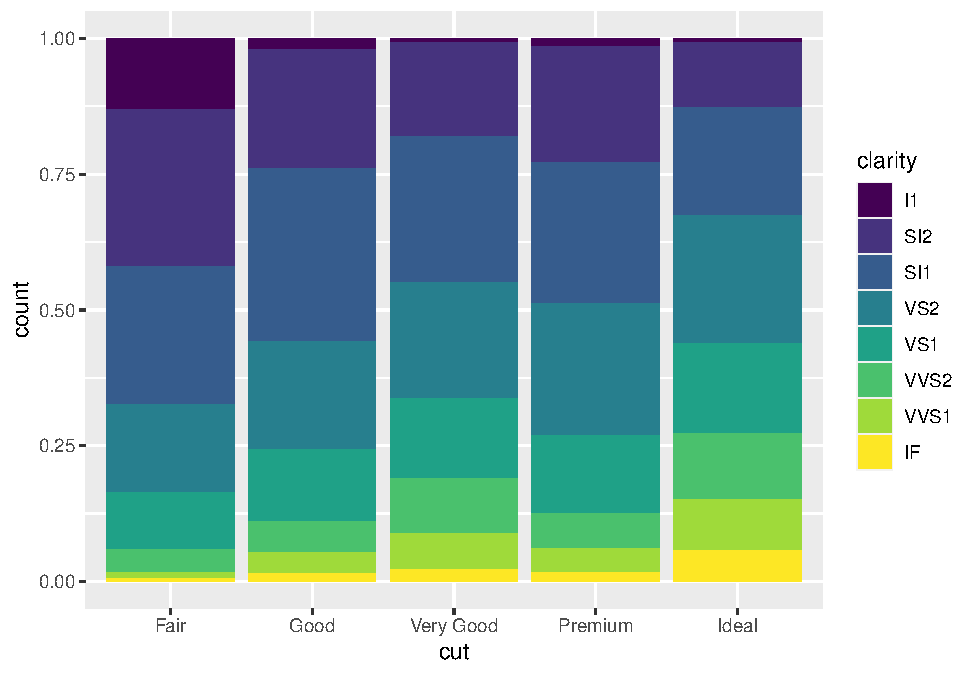
\includegraphics{Assignments_files/figure-latex/unnamed-chunk-50-1.pdf}
``position=fill'' makes each bar the same height for better comparison.

\begin{Shaded}
\begin{Highlighting}[]
\FunctionTok{ggplot}\NormalTok{(}\AttributeTok{data =}\NormalTok{ diamonds) }\SpecialCharTok{+} 
  \FunctionTok{geom\_bar}\NormalTok{(}\AttributeTok{mapping =} \FunctionTok{aes}\NormalTok{(}\AttributeTok{x =}\NormalTok{ cut, }\AttributeTok{fill =}\NormalTok{ clarity), }\AttributeTok{position =} \StringTok{"dodge"}\NormalTok{)}
\end{Highlighting}
\end{Shaded}

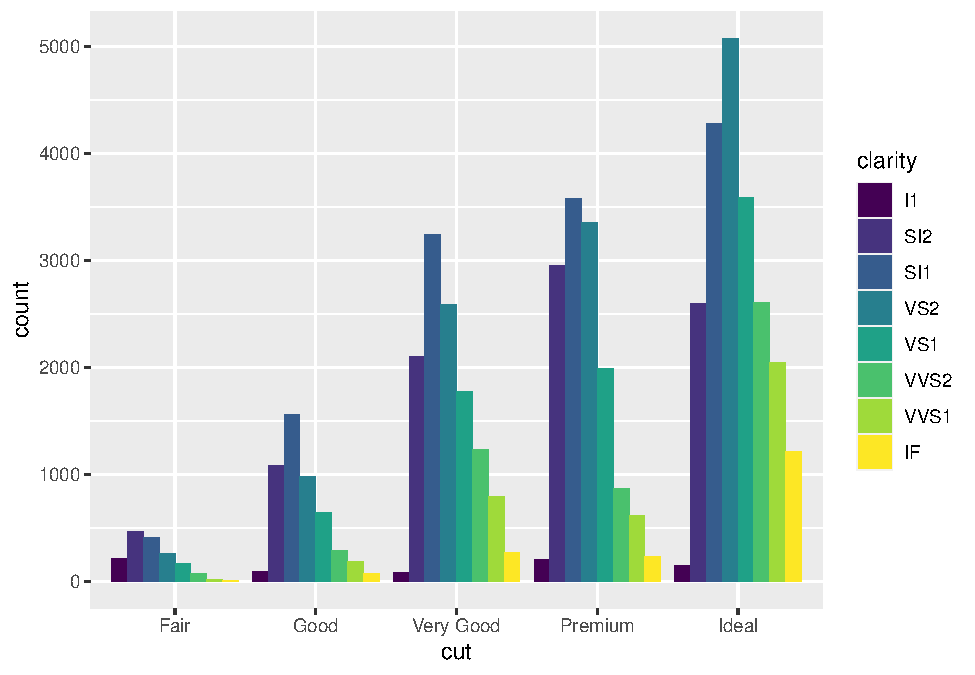
\includegraphics{Assignments_files/figure-latex/unnamed-chunk-51-1.pdf}
``position=dodge'' places overlapping objects beside each other

\begin{Shaded}
\begin{Highlighting}[]
\FunctionTok{ggplot}\NormalTok{(}\AttributeTok{data =}\NormalTok{ mpg) }\SpecialCharTok{+} 
  \FunctionTok{geom\_point}\NormalTok{(}\AttributeTok{mapping =} \FunctionTok{aes}\NormalTok{(}\AttributeTok{x =}\NormalTok{ displ, }\AttributeTok{y =}\NormalTok{ hwy), }\AttributeTok{position =} \StringTok{"jitter"}\NormalTok{)}
\end{Highlighting}
\end{Shaded}

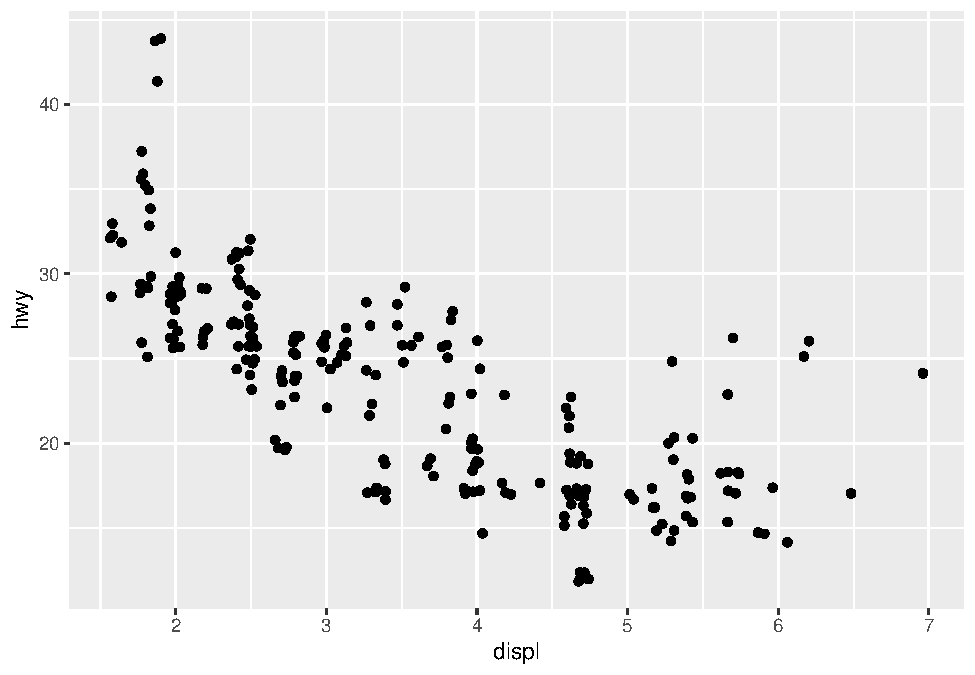
\includegraphics{Assignments_files/figure-latex/unnamed-chunk-52-1.pdf}
``position=jitter'' spreads the points out by adding random noise.

\begin{Shaded}
\begin{Highlighting}[]
\FunctionTok{ggplot}\NormalTok{(}\AttributeTok{data =}\NormalTok{ mpg, }\AttributeTok{mapping =} \FunctionTok{aes}\NormalTok{(}\AttributeTok{x =}\NormalTok{ class, }\AttributeTok{y =}\NormalTok{ hwy)) }\SpecialCharTok{+} 
  \FunctionTok{geom\_boxplot}\NormalTok{()}
\end{Highlighting}
\end{Shaded}

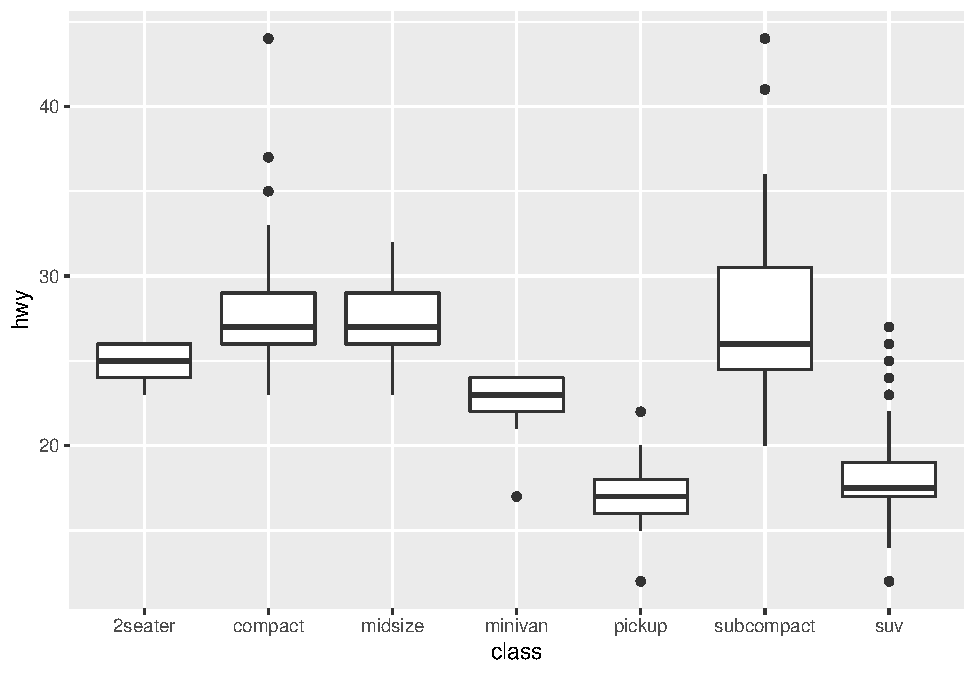
\includegraphics{Assignments_files/figure-latex/unnamed-chunk-53-1.pdf}

\begin{Shaded}
\begin{Highlighting}[]
\FunctionTok{ggplot}\NormalTok{(}\AttributeTok{data =}\NormalTok{ mpg, }\AttributeTok{mapping =} \FunctionTok{aes}\NormalTok{(}\AttributeTok{x =}\NormalTok{ class, }\AttributeTok{y =}\NormalTok{ hwy)) }\SpecialCharTok{+} 
  \FunctionTok{geom\_boxplot}\NormalTok{() }\SpecialCharTok{+}
  \FunctionTok{coord\_flip}\NormalTok{()}
\end{Highlighting}
\end{Shaded}

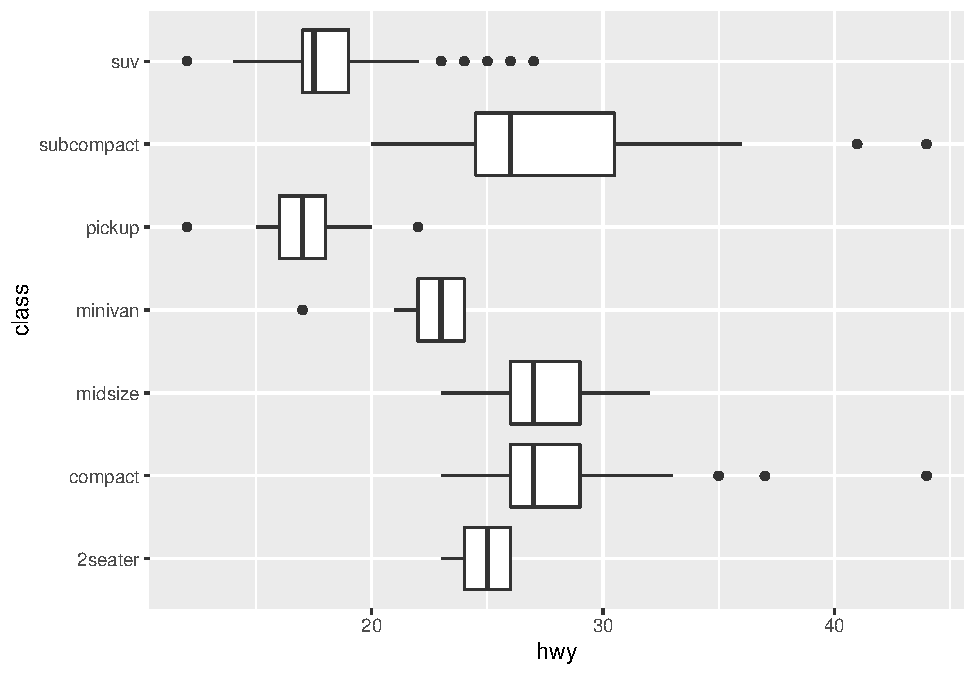
\includegraphics{Assignments_files/figure-latex/unnamed-chunk-53-2.pdf}
``coord\_filp'' flips the x and y axis.

\begin{Shaded}
\begin{Highlighting}[]
\NormalTok{nz }\OtherTok{\textless{}{-}} \FunctionTok{map\_data}\NormalTok{(}\StringTok{"nz"}\NormalTok{)}

\FunctionTok{ggplot}\NormalTok{(nz, }\FunctionTok{aes}\NormalTok{(long, lat, }\AttributeTok{group =}\NormalTok{ group)) }\SpecialCharTok{+}
  \FunctionTok{geom\_polygon}\NormalTok{(}\AttributeTok{fill =} \StringTok{"white"}\NormalTok{, }\AttributeTok{colour =} \StringTok{"black"}\NormalTok{)}
\end{Highlighting}
\end{Shaded}

\includegraphics{Assignments_files/figure-latex/unnamed-chunk-54-1.pdf}

\begin{Shaded}
\begin{Highlighting}[]
\FunctionTok{ggplot}\NormalTok{(nz, }\FunctionTok{aes}\NormalTok{(long, lat, }\AttributeTok{group =}\NormalTok{ group)) }\SpecialCharTok{+}
  \FunctionTok{geom\_polygon}\NormalTok{(}\AttributeTok{fill =} \StringTok{"white"}\NormalTok{, }\AttributeTok{colour =} \StringTok{"black"}\NormalTok{) }\SpecialCharTok{+}
  \FunctionTok{coord\_quickmap}\NormalTok{()}
\end{Highlighting}
\end{Shaded}

\includegraphics{Assignments_files/figure-latex/unnamed-chunk-54-2.pdf}
``coord\_quickmap'' sets the aspect ratio correctly for maps

\begin{Shaded}
\begin{Highlighting}[]
\NormalTok{bar }\OtherTok{\textless{}{-}} \FunctionTok{ggplot}\NormalTok{(}\AttributeTok{data =}\NormalTok{ diamonds) }\SpecialCharTok{+} 
  \FunctionTok{geom\_bar}\NormalTok{(}
    \AttributeTok{mapping =} \FunctionTok{aes}\NormalTok{(}\AttributeTok{x =}\NormalTok{ cut, }\AttributeTok{fill =}\NormalTok{ cut), }
    \AttributeTok{show.legend =} \ConstantTok{FALSE}\NormalTok{,}
    \AttributeTok{width =} \DecValTok{1}
\NormalTok{  ) }\SpecialCharTok{+} 
  \FunctionTok{theme}\NormalTok{(}\AttributeTok{aspect.ratio =} \DecValTok{1}\NormalTok{) }\SpecialCharTok{+}
  \FunctionTok{labs}\NormalTok{(}\AttributeTok{x =} \ConstantTok{NULL}\NormalTok{, }\AttributeTok{y =} \ConstantTok{NULL}\NormalTok{)}

\NormalTok{bar }\SpecialCharTok{+} \FunctionTok{coord\_flip}\NormalTok{()}
\end{Highlighting}
\end{Shaded}

\includegraphics{Assignments_files/figure-latex/unnamed-chunk-55-1.pdf}

\begin{Shaded}
\begin{Highlighting}[]
\NormalTok{bar }\SpecialCharTok{+} \FunctionTok{coord\_polar}\NormalTok{()}
\end{Highlighting}
\end{Shaded}

\includegraphics{Assignments_files/figure-latex/unnamed-chunk-55-2.pdf}
``coord\_polar'' uses polar coordinates which reveals a connection
between bar plots and a Coxcomb chart.

\begin{Shaded}
\begin{Highlighting}[]
\CommentTok{\#ggplot(data = \textless{}DATA\textgreater{}) + }
  \CommentTok{\#\textless{}GEOM\_FUNCTION\textgreater{}(}
     \CommentTok{\#mapping = aes(\textless{}MAPPINGS\textgreater{}),}
     \CommentTok{\#stat = \textless{}STAT\textgreater{}, }
     \CommentTok{\#position = \textless{}POSITION\textgreater{}}
  \CommentTok{\#) +}
  \CommentTok{\#\textless{}COORDINATE\_FUNCTION\textgreater{} +}
  \CommentTok{\#\textless{}FACET\_FUNCTION\textgreater{}}
\end{Highlighting}
\end{Shaded}

Rough template for making ggplots

\hypertarget{graphics-for-communication}{%
\subsubsection{Graphics for
Communication}\label{graphics-for-communication}}

\begin{Shaded}
\begin{Highlighting}[]
\FunctionTok{ggplot}\NormalTok{(mpg, }\FunctionTok{aes}\NormalTok{(displ, hwy)) }\SpecialCharTok{+}
  \FunctionTok{geom\_point}\NormalTok{(}\FunctionTok{aes}\NormalTok{(}\AttributeTok{color =}\NormalTok{ class)) }\SpecialCharTok{+}
  \FunctionTok{geom\_smooth}\NormalTok{(}\AttributeTok{se =} \ConstantTok{FALSE}\NormalTok{) }\SpecialCharTok{+}
  \FunctionTok{labs}\NormalTok{(}\AttributeTok{title =} \StringTok{"Fuel efficiency generally decreases with engine size"}\NormalTok{,}
    \AttributeTok{subtitle =} \StringTok{"Two seaters (sports cars) are an exception because of their light weight"}\NormalTok{,}
    \AttributeTok{caption =} \StringTok{"Data from fueleconomy.gov"}\NormalTok{,}
    \AttributeTok{x =} \StringTok{"Engine displacement (L)"}\NormalTok{,}
    \AttributeTok{y =} \StringTok{"Highway fuel economy (mpg)"}\NormalTok{,}
    \AttributeTok{colour =} \StringTok{"Car type"}\NormalTok{)}
\end{Highlighting}
\end{Shaded}

\begin{verbatim}
## `geom_smooth()` using method = 'loess' and formula 'y ~ x'
\end{verbatim}

\includegraphics{Assignments_files/figure-latex/unnamed-chunk-57-1.pdf}
the "labs() function adds labels to your plots. Title is the main name
of the plot, subtitle is used to add details about the plot under the
title and caption adds more detail under the plot usually used to
indicate the source if the data.the x and y axis can also be labeled
under this function.

\begin{Shaded}
\begin{Highlighting}[]
\NormalTok{best\_in\_class }\OtherTok{\textless{}{-}}\NormalTok{ mpg }\SpecialCharTok{\%\textgreater{}\%}
  \FunctionTok{group\_by}\NormalTok{(class) }\SpecialCharTok{\%\textgreater{}\%}
  \FunctionTok{filter}\NormalTok{(}\FunctionTok{row\_number}\NormalTok{(}\FunctionTok{desc}\NormalTok{(hwy)) }\SpecialCharTok{==} \DecValTok{1}\NormalTok{)}

\FunctionTok{ggplot}\NormalTok{(mpg, }\FunctionTok{aes}\NormalTok{(displ, hwy)) }\SpecialCharTok{+}
  \FunctionTok{geom\_point}\NormalTok{(}\FunctionTok{aes}\NormalTok{(}\AttributeTok{colour =}\NormalTok{ class)) }\SpecialCharTok{+}
  \FunctionTok{geom\_label}\NormalTok{(}\FunctionTok{aes}\NormalTok{(}\AttributeTok{label =}\NormalTok{ model), }\AttributeTok{data =}\NormalTok{ best\_in\_class, }\AttributeTok{nudge\_y =} \DecValTok{2}\NormalTok{, }\AttributeTok{alpha =} \FloatTok{0.5}\NormalTok{)}
\end{Highlighting}
\end{Shaded}

\includegraphics{Assignments_files/figure-latex/unnamed-chunk-58-1.pdf}
The best in class function choses the most effecient cars in the data
and the functions ``geom\_text()'' and ``geom\_text()'' provides labels
to the points. The function geom\_label() makes the label clearer by
drawing a rectangle behind the text and nudge\_y moves the label so it
can be viewed clearer.

\begin{Shaded}
\begin{Highlighting}[]
\CommentTok{\#install.packages("ggrepel")}
\FunctionTok{ggplot}\NormalTok{(mpg, }\FunctionTok{aes}\NormalTok{(displ, hwy)) }\SpecialCharTok{+}
  \FunctionTok{geom\_point}\NormalTok{(}\FunctionTok{aes}\NormalTok{(}\AttributeTok{colour =}\NormalTok{ class)) }\SpecialCharTok{+}
  \FunctionTok{geom\_point}\NormalTok{(}\AttributeTok{size =} \DecValTok{3}\NormalTok{, }\AttributeTok{shape =} \DecValTok{1}\NormalTok{, }\AttributeTok{data =}\NormalTok{ best\_in\_class) }\SpecialCharTok{+}
\NormalTok{  ggrepel}\SpecialCharTok{::}\FunctionTok{geom\_label\_repel}\NormalTok{(}\FunctionTok{aes}\NormalTok{(}\AttributeTok{label =}\NormalTok{ model), }\AttributeTok{data =}\NormalTok{ best\_in\_class)}
\end{Highlighting}
\end{Shaded}

\includegraphics{Assignments_files/figure-latex/unnamed-chunk-59-1.pdf}
This is another way to add labels to the graphs. Using the package
ggrepel, we can automatically add labels that do not overlap.

\begin{Shaded}
\begin{Highlighting}[]
\NormalTok{class\_avg }\OtherTok{\textless{}{-}}\NormalTok{ mpg }\SpecialCharTok{\%\textgreater{}\%}
  \FunctionTok{group\_by}\NormalTok{(class) }\SpecialCharTok{\%\textgreater{}\%}
  \FunctionTok{summarise}\NormalTok{(}
    \AttributeTok{displ =} \FunctionTok{median}\NormalTok{(displ),}
    \AttributeTok{hwy =} \FunctionTok{median}\NormalTok{(hwy)}
\NormalTok{  )}
\CommentTok{\#\textgreater{} \textasciigrave{}summarise()\textasciigrave{} ungrouping output (override with \textasciigrave{}.groups\textasciigrave{} argument)}

\FunctionTok{ggplot}\NormalTok{(mpg, }\FunctionTok{aes}\NormalTok{(displ, hwy, }\AttributeTok{colour =}\NormalTok{ class)) }\SpecialCharTok{+}
\NormalTok{  ggrepel}\SpecialCharTok{::}\FunctionTok{geom\_label\_repel}\NormalTok{(}\FunctionTok{aes}\NormalTok{(}\AttributeTok{label =}\NormalTok{ class),}
    \AttributeTok{data =}\NormalTok{ class\_avg,}
    \AttributeTok{size =} \DecValTok{6}\NormalTok{,}
    \AttributeTok{label.size =} \DecValTok{0}\NormalTok{,}
    \AttributeTok{segment.color =} \ConstantTok{NA}
\NormalTok{  ) }\SpecialCharTok{+}
  \FunctionTok{geom\_point}\NormalTok{() }\SpecialCharTok{+}
  \FunctionTok{theme}\NormalTok{(}\AttributeTok{legend.position =} \StringTok{"none"}\NormalTok{)}
\end{Highlighting}
\end{Shaded}

\includegraphics{Assignments_files/figure-latex/unnamed-chunk-60-1.pdf}
This code replaces the legend with labels that are directly on the plot.

\begin{Shaded}
\begin{Highlighting}[]
\NormalTok{label }\OtherTok{\textless{}{-}}\NormalTok{ mpg }\SpecialCharTok{\%\textgreater{}\%}
  \FunctionTok{summarise}\NormalTok{(}
    \AttributeTok{displ =} \FunctionTok{max}\NormalTok{(displ),}
    \AttributeTok{hwy =} \FunctionTok{max}\NormalTok{(hwy),}
    \AttributeTok{label =} \StringTok{"Increasing engine size is }\SpecialCharTok{\textbackslash{}n}\StringTok{related to decreasing fuel economy."}
\NormalTok{  )}

\FunctionTok{ggplot}\NormalTok{(mpg, }\FunctionTok{aes}\NormalTok{(displ, hwy)) }\SpecialCharTok{+}
  \FunctionTok{geom\_point}\NormalTok{() }\SpecialCharTok{+}
  \FunctionTok{geom\_text}\NormalTok{(}\FunctionTok{aes}\NormalTok{(}\AttributeTok{label =}\NormalTok{ label), }\AttributeTok{data =}\NormalTok{ label, }\AttributeTok{vjust =} \StringTok{"top"}\NormalTok{, }\AttributeTok{hjust =} \StringTok{"right"}\NormalTok{)}
\end{Highlighting}
\end{Shaded}

\includegraphics{Assignments_files/figure-latex/unnamed-chunk-61-1.pdf}
A new data frame is created using summarise() so a single label can be
added to the plot. geom\_hline(), geom\_vline(), thick (size = 2) and
white (colour = white) can be used to add reference lines.geom\_rect()
is used to draw rectangles around points of interest. geom\_segment with
an arrow argument emphasizes a point with an arrow.

\begin{Shaded}
\begin{Highlighting}[]
\FunctionTok{ggplot}\NormalTok{(mpg, }\FunctionTok{aes}\NormalTok{(displ, hwy)) }\SpecialCharTok{+}
  \FunctionTok{geom\_point}\NormalTok{() }\SpecialCharTok{+}
  \FunctionTok{scale\_y\_continuous}\NormalTok{(}\AttributeTok{breaks =} \FunctionTok{seq}\NormalTok{(}\DecValTok{15}\NormalTok{, }\DecValTok{40}\NormalTok{, }\AttributeTok{by =} \DecValTok{5}\NormalTok{))}
\end{Highlighting}
\end{Shaded}

\includegraphics{Assignments_files/figure-latex/unnamed-chunk-62-1.pdf}
"breaks' controls the positions of the ticks on the plot. This code
overrides the default break choice.

\begin{Shaded}
\begin{Highlighting}[]
\FunctionTok{ggplot}\NormalTok{(mpg, }\FunctionTok{aes}\NormalTok{(displ, hwy)) }\SpecialCharTok{+}
  \FunctionTok{geom\_point}\NormalTok{() }\SpecialCharTok{+}
  \FunctionTok{scale\_x\_continuous}\NormalTok{(}\AttributeTok{labels =} \ConstantTok{NULL}\NormalTok{) }\SpecialCharTok{+}
  \FunctionTok{scale\_y\_continuous}\NormalTok{(}\AttributeTok{labels =} \ConstantTok{NULL}\NormalTok{)}
\end{Highlighting}
\end{Shaded}

\includegraphics{Assignments_files/figure-latex/unnamed-chunk-63-1.pdf}
Using labels and null hides the labels (in this case the numbers) on the
axis. This is useful for maps.

\begin{Shaded}
\begin{Highlighting}[]
\NormalTok{base }\OtherTok{\textless{}{-}} \FunctionTok{ggplot}\NormalTok{(mpg, }\FunctionTok{aes}\NormalTok{(displ, hwy)) }\SpecialCharTok{+}
  \FunctionTok{geom\_point}\NormalTok{(}\FunctionTok{aes}\NormalTok{(}\AttributeTok{colour =}\NormalTok{ class))}

\NormalTok{base }\SpecialCharTok{+} \FunctionTok{theme}\NormalTok{(}\AttributeTok{legend.position =} \StringTok{"left"}\NormalTok{)}
\end{Highlighting}
\end{Shaded}

\includegraphics{Assignments_files/figure-latex/unnamed-chunk-64-1.pdf}

\begin{Shaded}
\begin{Highlighting}[]
\NormalTok{base }\SpecialCharTok{+} \FunctionTok{theme}\NormalTok{(}\AttributeTok{legend.position =} \StringTok{"top"}\NormalTok{)}
\end{Highlighting}
\end{Shaded}

\includegraphics{Assignments_files/figure-latex/unnamed-chunk-64-2.pdf}

\begin{Shaded}
\begin{Highlighting}[]
\NormalTok{base }\SpecialCharTok{+} \FunctionTok{theme}\NormalTok{(}\AttributeTok{legend.position =} \StringTok{"bottom"}\NormalTok{)}
\end{Highlighting}
\end{Shaded}

\includegraphics{Assignments_files/figure-latex/unnamed-chunk-64-3.pdf}

\begin{Shaded}
\begin{Highlighting}[]
\NormalTok{base }\SpecialCharTok{+} \FunctionTok{theme}\NormalTok{(}\AttributeTok{legend.position =} \StringTok{"right"}\NormalTok{) }\CommentTok{\# the default}
\end{Highlighting}
\end{Shaded}

\includegraphics{Assignments_files/figure-latex/unnamed-chunk-64-4.pdf}
``theme()'' is used to control the non-data parts of the plot so this
code controls where the legend is drawn.

\begin{Shaded}
\begin{Highlighting}[]
\FunctionTok{ggplot}\NormalTok{(mpg, }\FunctionTok{aes}\NormalTok{(displ, hwy)) }\SpecialCharTok{+}
  \FunctionTok{geom\_point}\NormalTok{(}\FunctionTok{aes}\NormalTok{(}\AttributeTok{colour =}\NormalTok{ class)) }\SpecialCharTok{+}
  \FunctionTok{geom\_smooth}\NormalTok{(}\AttributeTok{se =} \ConstantTok{FALSE}\NormalTok{) }\SpecialCharTok{+}
  \FunctionTok{theme}\NormalTok{(}\AttributeTok{legend.position =} \StringTok{"bottom"}\NormalTok{) }\SpecialCharTok{+}
  \FunctionTok{guides}\NormalTok{(}\AttributeTok{colour =} \FunctionTok{guide\_legend}\NormalTok{(}\AttributeTok{nrow =} \DecValTok{1}\NormalTok{, }\AttributeTok{override.aes =} \FunctionTok{list}\NormalTok{(}\AttributeTok{size =} \DecValTok{4}\NormalTok{)))}
\end{Highlighting}
\end{Shaded}

\begin{verbatim}
## `geom_smooth()` using method = 'loess' and formula 'y ~ x'
\end{verbatim}

\includegraphics{Assignments_files/figure-latex/unnamed-chunk-65-1.pdf}

\begin{Shaded}
\begin{Highlighting}[]
\CommentTok{\#\textgreater{} \textasciigrave{}geom\_smooth()\textasciigrave{} using method = \textquotesingle{}loess\textquotesingle{} and formula \textquotesingle{}y \textasciitilde{} x\textquotesingle{}}
\end{Highlighting}
\end{Shaded}

This code controls the number of rows in the legend and makes the points
bigger.

\begin{Shaded}
\begin{Highlighting}[]
\FunctionTok{ggplot}\NormalTok{(diamonds, }\FunctionTok{aes}\NormalTok{(carat, price)) }\SpecialCharTok{+}
  \FunctionTok{geom\_bin2d}\NormalTok{() }\SpecialCharTok{+} 
  \FunctionTok{scale\_x\_log10}\NormalTok{() }\SpecialCharTok{+} 
  \FunctionTok{scale\_y\_log10}\NormalTok{()}
\end{Highlighting}
\end{Shaded}

\includegraphics{Assignments_files/figure-latex/unnamed-chunk-66-1.pdf}
Transform the data using scale so the labels on the axis stay the same.

\begin{Shaded}
\begin{Highlighting}[]
\FunctionTok{ggplot}\NormalTok{(mpg, }\FunctionTok{aes}\NormalTok{(displ, hwy)) }\SpecialCharTok{+}
  \FunctionTok{geom\_point}\NormalTok{(}\FunctionTok{aes}\NormalTok{(}\AttributeTok{color =}\NormalTok{ drv))}
\end{Highlighting}
\end{Shaded}

\includegraphics{Assignments_files/figure-latex/unnamed-chunk-67-1.pdf}

\begin{Shaded}
\begin{Highlighting}[]
\FunctionTok{ggplot}\NormalTok{(mpg, }\FunctionTok{aes}\NormalTok{(displ, hwy)) }\SpecialCharTok{+}
  \FunctionTok{geom\_point}\NormalTok{(}\FunctionTok{aes}\NormalTok{(}\AttributeTok{color =}\NormalTok{ drv, }\AttributeTok{shape =}\NormalTok{ drv)) }\SpecialCharTok{+}
  \FunctionTok{scale\_colour\_brewer}\NormalTok{(}\AttributeTok{palette =} \StringTok{"Set1"}\NormalTok{)}
\end{Highlighting}
\end{Shaded}

\includegraphics{Assignments_files/figure-latex/unnamed-chunk-67-2.pdf}
ColorBrewer scales are colors that are easy to interpret for people with
common types of color blindness. The shape function adds redundant shape
mapping to the plot so it can be easily interpreted in black and white.

\begin{Shaded}
\begin{Highlighting}[]
\NormalTok{presidential }\SpecialCharTok{\%\textgreater{}\%}
  \FunctionTok{mutate}\NormalTok{(}\AttributeTok{id =} \DecValTok{33} \SpecialCharTok{+} \FunctionTok{row\_number}\NormalTok{()) }\SpecialCharTok{\%\textgreater{}\%}
  \FunctionTok{ggplot}\NormalTok{(}\FunctionTok{aes}\NormalTok{(start, id, }\AttributeTok{colour =}\NormalTok{ party)) }\SpecialCharTok{+}
    \FunctionTok{geom\_point}\NormalTok{() }\SpecialCharTok{+}
    \FunctionTok{geom\_segment}\NormalTok{(}\FunctionTok{aes}\NormalTok{(}\AttributeTok{xend =}\NormalTok{ end, }\AttributeTok{yend =}\NormalTok{ id)) }\SpecialCharTok{+}
    \FunctionTok{scale\_colour\_manual}\NormalTok{(}\AttributeTok{values =} \FunctionTok{c}\NormalTok{(}\AttributeTok{Republican =} \StringTok{"red"}\NormalTok{, }\AttributeTok{Democratic =} \StringTok{"blue"}\NormalTok{))}
\end{Highlighting}
\end{Shaded}

\includegraphics{Assignments_files/figure-latex/unnamed-chunk-68-1.pdf}
``scale\_colour\_manual()'' is used for predefined mapping between
values. Here it makes Republican presidents red and Democratic
presidents blue.

\begin{Shaded}
\begin{Highlighting}[]
\FunctionTok{ggplot}\NormalTok{(mpg, }\AttributeTok{mapping =} \FunctionTok{aes}\NormalTok{(displ, hwy)) }\SpecialCharTok{+}
  \FunctionTok{geom\_point}\NormalTok{(}\FunctionTok{aes}\NormalTok{(}\AttributeTok{color =}\NormalTok{ class)) }\SpecialCharTok{+}
  \FunctionTok{geom\_smooth}\NormalTok{() }\SpecialCharTok{+}
  \FunctionTok{coord\_cartesian}\NormalTok{(}\AttributeTok{xlim =} \FunctionTok{c}\NormalTok{(}\DecValTok{5}\NormalTok{, }\DecValTok{7}\NormalTok{), }\AttributeTok{ylim =} \FunctionTok{c}\NormalTok{(}\DecValTok{10}\NormalTok{, }\DecValTok{30}\NormalTok{))}
\end{Highlighting}
\end{Shaded}

\begin{verbatim}
## `geom_smooth()` using method = 'loess' and formula 'y ~ x'
\end{verbatim}

\includegraphics{Assignments_files/figure-latex/unnamed-chunk-69-1.pdf}

\begin{Shaded}
\begin{Highlighting}[]
\NormalTok{mpg }\SpecialCharTok{\%\textgreater{}\%}
  \FunctionTok{filter}\NormalTok{(displ }\SpecialCharTok{\textgreater{}=} \DecValTok{5}\NormalTok{, displ }\SpecialCharTok{\textless{}=} \DecValTok{7}\NormalTok{, hwy }\SpecialCharTok{\textgreater{}=} \DecValTok{10}\NormalTok{, hwy }\SpecialCharTok{\textless{}=} \DecValTok{30}\NormalTok{) }\SpecialCharTok{\%\textgreater{}\%}
  \FunctionTok{ggplot}\NormalTok{(}\FunctionTok{aes}\NormalTok{(displ, hwy)) }\SpecialCharTok{+}
  \FunctionTok{geom\_point}\NormalTok{(}\FunctionTok{aes}\NormalTok{(}\AttributeTok{color =}\NormalTok{ class)) }\SpecialCharTok{+}
  \FunctionTok{geom\_smooth}\NormalTok{()}
\end{Highlighting}
\end{Shaded}

\begin{verbatim}
## `geom_smooth()` using method = 'loess' and formula 'y ~ x'
\end{verbatim}

\includegraphics{Assignments_files/figure-latex/unnamed-chunk-69-2.pdf}
``coord\_cartesian()'' zooms into one region of the plot.

\begin{Shaded}
\begin{Highlighting}[]
\NormalTok{suv }\OtherTok{\textless{}{-}}\NormalTok{ mpg }\SpecialCharTok{\%\textgreater{}\%} \FunctionTok{filter}\NormalTok{(class }\SpecialCharTok{==} \StringTok{"suv"}\NormalTok{)}
\NormalTok{compact }\OtherTok{\textless{}{-}}\NormalTok{ mpg }\SpecialCharTok{\%\textgreater{}\%} \FunctionTok{filter}\NormalTok{(class }\SpecialCharTok{==} \StringTok{"compact"}\NormalTok{)}

\FunctionTok{ggplot}\NormalTok{(suv, }\FunctionTok{aes}\NormalTok{(displ, hwy, }\AttributeTok{colour =}\NormalTok{ drv)) }\SpecialCharTok{+}
  \FunctionTok{geom\_point}\NormalTok{()}
\end{Highlighting}
\end{Shaded}

\includegraphics{Assignments_files/figure-latex/unnamed-chunk-70-1.pdf}

\begin{Shaded}
\begin{Highlighting}[]
\FunctionTok{ggplot}\NormalTok{(compact, }\FunctionTok{aes}\NormalTok{(displ, hwy, }\AttributeTok{colour =}\NormalTok{ drv)) }\SpecialCharTok{+}
  \FunctionTok{geom\_point}\NormalTok{()}
\end{Highlighting}
\end{Shaded}

\includegraphics{Assignments_files/figure-latex/unnamed-chunk-70-2.pdf}
Plotting two classes of cars and plotting them seperatly.

\begin{Shaded}
\begin{Highlighting}[]
\NormalTok{x\_scale }\OtherTok{\textless{}{-}} \FunctionTok{scale\_x\_continuous}\NormalTok{(}\AttributeTok{limits =} \FunctionTok{range}\NormalTok{(mpg}\SpecialCharTok{$}\NormalTok{displ))}
\NormalTok{y\_scale }\OtherTok{\textless{}{-}} \FunctionTok{scale\_y\_continuous}\NormalTok{(}\AttributeTok{limits =} \FunctionTok{range}\NormalTok{(mpg}\SpecialCharTok{$}\NormalTok{hwy))}
\NormalTok{col\_scale }\OtherTok{\textless{}{-}} \FunctionTok{scale\_colour\_discrete}\NormalTok{(}\AttributeTok{limits =} \FunctionTok{unique}\NormalTok{(mpg}\SpecialCharTok{$}\NormalTok{drv))}

\FunctionTok{ggplot}\NormalTok{(suv, }\FunctionTok{aes}\NormalTok{(displ, hwy, }\AttributeTok{colour =}\NormalTok{ drv)) }\SpecialCharTok{+}
  \FunctionTok{geom\_point}\NormalTok{() }\SpecialCharTok{+}
\NormalTok{  x\_scale }\SpecialCharTok{+}
\NormalTok{  y\_scale }\SpecialCharTok{+}
\NormalTok{  col\_scale}
\end{Highlighting}
\end{Shaded}

\includegraphics{Assignments_files/figure-latex/unnamed-chunk-71-1.pdf}

\begin{Shaded}
\begin{Highlighting}[]
\FunctionTok{ggplot}\NormalTok{(compact, }\FunctionTok{aes}\NormalTok{(displ, hwy, }\AttributeTok{colour =}\NormalTok{ drv)) }\SpecialCharTok{+}
  \FunctionTok{geom\_point}\NormalTok{() }\SpecialCharTok{+}
\NormalTok{  x\_scale }\SpecialCharTok{+}
\NormalTok{  y\_scale }\SpecialCharTok{+}
\NormalTok{  col\_scale}
\end{Highlighting}
\end{Shaded}

\includegraphics{Assignments_files/figure-latex/unnamed-chunk-71-2.pdf}
When two datasets have different scales, ``limits'' can be used to make
them equal so they can be compared.

\begin{Shaded}
\begin{Highlighting}[]
\FunctionTok{ggplot}\NormalTok{(mpg, }\FunctionTok{aes}\NormalTok{(displ, hwy)) }\SpecialCharTok{+}
  \FunctionTok{geom\_point}\NormalTok{(}\FunctionTok{aes}\NormalTok{(}\AttributeTok{color =}\NormalTok{ class)) }\SpecialCharTok{+}
  \FunctionTok{geom\_smooth}\NormalTok{(}\AttributeTok{se =} \ConstantTok{FALSE}\NormalTok{) }\SpecialCharTok{+}
  \FunctionTok{theme\_bw}\NormalTok{()}
\end{Highlighting}
\end{Shaded}

\begin{verbatim}
## `geom_smooth()` using method = 'loess' and formula 'y ~ x'
\end{verbatim}

\includegraphics{Assignments_files/figure-latex/unnamed-chunk-72-1.pdf}
Adds a theme for the non-data elements of the plot. There are 8 themes
by default.

\begin{Shaded}
\begin{Highlighting}[]
\FunctionTok{ggplot}\NormalTok{(mpg, }\FunctionTok{aes}\NormalTok{(displ, hwy)) }\SpecialCharTok{+} \FunctionTok{geom\_point}\NormalTok{()}
\end{Highlighting}
\end{Shaded}

\includegraphics{Assignments_files/figure-latex/unnamed-chunk-73-1.pdf}

\begin{Shaded}
\begin{Highlighting}[]
\FunctionTok{ggsave}\NormalTok{(}\StringTok{"my{-}plot.pdf"}\NormalTok{)}
\end{Highlighting}
\end{Shaded}

\begin{verbatim}
## Saving 6.5 x 4.5 in image
\end{verbatim}

\begin{Shaded}
\begin{Highlighting}[]
\CommentTok{\#\textgreater{} Saving 7 x 4.33 in image}
\end{Highlighting}
\end{Shaded}

This code saves your ggplot. You can specify width and height but if you
do not specify it will save as the dimensions of the current plotting
device. To make plots have a consistent width use ``fig.width'' and
fig.asp``. fig.width = 6 (6'') and fig.asp = 0.618 is the golden ratio
and can be set in the defaults. out.width = ``70\%'' and fig.align =
``center'' is used to control output size. For multiple plots in a row
use out.width to 50\% for two plots, 33\% for 3 plots, or 25\% to 4
plots, and set fig.align = ``default''.

\end{document}
